\documentclass[aspectratio=169]{beamer}
\usepackage{hyperref}
\usepackage[T1]{fontenc}
\usepackage{newtxtext,newtxmath}
\makeatletter
\def\input@path{{}{3. Presentacion/}}
\makeatother
\usepackage{tribhuvan}
\usepackage[absolute,overlay]{textpos}
\usepackage[table]{xcolor}

% Color para distintivos de contribución (Rojo llamativo)
\definecolor{colorRojoContrib}{rgb}{0.85, 0.12, 0.15} 
% Color azul para filas de propuesta en tablas
\definecolor{azulPropuesta}{RGB}{20, 55, 108}
\definecolor{llamativoMagenta}{rgb}{0.85, 0.12, 0.15}
\newcommand{\contrib}[1]{\textcolor{colorRojoContrib}{\textbf{\underline{#1}}}}


% other packages
\usepackage{latexsym,amsmath,xcolor,multicol,booktabs,calligra}
\usepackage{graphicx,pstricks,listings,stackengine}
\graphicspath{{figures_optimized/}{../figures_optimized/}{../../figures_optimized/}{figures/}{../figures/}{../../figures/}}
\makeatletter
\newcounter{prismfigure}
\renewcommand{\theprismfigure}{\arabic{prismfigure}}
\providecommand{\theHprismfigure}{\arabic{prismfigure}}
\let\prism@original@includegraphics\includegraphics
\renewcommand{\includegraphics}[2][]{%
    \prism@original@includegraphics[#1]{#2}%
    \refstepcounter{prismfigure}%
    \label{fig:auto-\theprismfigure}%
}
\makeatother

\author[Carlos Benítez, carlosbenitez@fiuna.edu.py, FIUNA]{Carlos Benítez}
\title[33ª Jornadas de Jovens Pesquisadores (AUGM) -- UFRGS]{Avanços do protótipo de processamento local para detecção, classificação e análise preditiva de manchas solares}
\subtitle{Relatório de avanço para tutoria}
\institute[]{Universidad Nacional de Asunción \\ Facultad de Ingeniería \\ Engenharia Mecatrônica}
\date{13 de abril de 2026}


% defs
\def\cmd#1{\texttt{\color{red}\footnotesize $\backslash$#1}}
\def\env#1{\texttt{\color{blue}\footnotesize #1}}
\definecolor{deepblue}{rgb}{0,0,0.5}
\definecolor{deepred}{rgb}{0.6,0,0}
\definecolor{deepgreen}{rgb}{0,0.5,0}
\definecolor{halfgray}{gray}{0.55}

\lstset{
    basicstyle=\ttfamily\small,
    keywordstyle=\bfseries\color{deepblue},
    emphstyle=\ttfamily\color{deepred},    % Custom highlighting style
    stringstyle=\color{deepgreen},
    numbers=left,
    numberstyle=\small\color{halfgray},
    rulesepcolor=\color{red!20!green!20!blue!20},
    frame=shadowbox,
}

\renewcommand{\familydefault}{\rmdefault}
\setbeamerfont{title}{size=\Large}
\setbeamerfont{subtitle}{size=\normalsize}
\setbeamerfont{author}{size=\normalsize}
\setbeamerfont{institute}{size=\small}
\setbeamerfont{date}{size=\small}

\newcommand{\imageplaceholder}[2][0.95\linewidth]{%
    \fbox{%
        \begin{minipage}[c][0.20\textheight][c]{#1}
            \centering
            \textbf{[Imagem pendente]}\\[4pt]
            \footnotesize #2
        \end{minipage}%
    }%
}

\AtBeginSection[]{}
\AtBeginSubsection[]{}


\begin{document}

\begin{frame}[plain]
    \centering
    \vspace*{0.28cm}

    % --- CABECERA INSTITUCIONAL: Sellos sutiles en los extremos ---
    \noindent
    \parbox[c]{0.48\linewidth}{%
        
\includegraphics[height=0.82cm,keepaspectratio]{una_logo.png}\hspace{0.25cm}%
        
\includegraphics[height=0.92cm,keepaspectratio]{logos/fiuna_logo.png}%
    }%
    \hfill
    \parbox[c]{0.48\linewidth}{%
        \raggedleft
        
\includegraphics[height=0.92cm,keepaspectratio]{logos/observario_logo.png}\hspace{0.18cm}%
        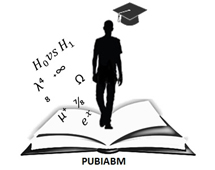
\includegraphics[height=1.08cm,keepaspectratio]{logos/pubiam_logo.jpg}%
    }
    
    \vspace{0.12cm}
    {\color{granate!20}\rule{\linewidth}{0.6pt}}
    \vspace{0.25cm}

    % --- CUERPO PRINCIPAL HERO (Layout 16:9 Panorámico Armonioso) ---
    \begin{columns}[c, onlytextwidth]
        % COLUMNA IZQUIERDA: Título protagónico, autor y coautores
        \begin{column}{0.59\textwidth}
            {\scriptsize\bfseries\color{granate} 33ª JORNADAS DE JOVENS PESQUISADORES $\cdot$ AUGM 2026\par}
            \vspace{0.12cm}
            {\large\bfseries\color{rojo-oscuro} Desenvolvimento de um Protótipo de Processamento Local para Detecção, Classificação e Análise Preditiva de Manchas Solares mediante Visão Computacional e IA\par}
            
            \vspace{0.14cm}
            {\color{linea-progreso}\rule{0.50\linewidth}{1.6pt}\par}
            \vspace{0.22cm}

            {\normalsize\textbf{Carlos Benítez}\par}
            \vspace{0.04cm}
            {\footnotesize\color{black!80} Universidad Nacional de Asunción $\cdot$ Facultad de Ingeniería\par}
            {\scriptsize\color{black!60} Engenharia Mecatrônica\par}

            \vspace{0.25cm}
            {\footnotesize\textbf{\color{rojo-oscuro}Coautores:}\\[2pt]
            \footnotesize\color{black!85}
            Dr. Juan Carlos Cabral \quad$\cdot$\quad Dr. Diego Stalder\\[2pt]
            Dr. Christian E. Schaerer \quad$\cdot$\quad Dr. José María Gómez\\[2pt]
            MSc. Jesús Núñez\par}
        \end{column}

        % COLUMNA DERECHA: Logo del evento con MÁXIMO PROTAGONISMO Y ARMONÍA
        \begin{column}{0.39\textwidth}
            \centering
            
\includegraphics[width=\linewidth,height=4.6cm,keepaspectratio]{logos/v1_color.png}
        \end{column}
    \end{columns}

    \vfill
    \vspace{0.1cm}
\end{frame}

% --- FRAME 1: Beca PUBIABM (Denominación Oficial) ---
% \begin{frame}{Agradecimientos Institucionales}
%     \begin{columns}[c]
%         \begin{column}{0.35\textwidth}
%             \centering
%             
\includegraphics[width=\textwidth]{logos/pubiam_logo.png}
%         \end{column}
        
%         \begin{column}{0.60\textwidth}
%             \small
%             \textit{Se expresa el reconocimiento formal al \textbf{Programa Universitario de Becas para la Investigación Académica "Andrés Borgognon Montero" (PUBIABM) y a la Empresa Ganadera 13 de Mayo S.A.} por el apoyo financiero}
            
%             \vspace{0.3em}
%             \textit{Los recursos económicos provistos por dicho fondo permitieron solventar los costos de adquisición de insumos de hardware especializados, así como los componentes de instrumentación electrónica que resultaron esenciales para el desarrollo metodológico y el ensamblaje del prototipo.}
%         \end{column}
%     \end{columns}
% \end{frame}

% % --- FRAME 2: Observatorio Alexis Troche Boggino ---
% \begin{frame}{Agradecimientos Institucionales}
%     \begin{columns}[c]
%         \begin{column}{0.4\textwidth}
%             \centering
%             
\includegraphics[width=\textwidth]{logos/observario_logo.png}
%         \end{column}
        
%         \begin{column}{0.50\textwidth}
%             \small
%             \textit{Se extiende el agradecimiento institucional al \textbf{Observatorio Astronómico "Prof. Alexis Troche Boggino" de la Facultad Politécnica de la Universidad Nacional de Asunción}, por la autorización y apertura de sus instalaciones.}
%         \end{column}
%     \end{columns}
% \end{frame}

\begin{frame}
    \centering
    \vfill
    \begin{minipage}{0.85\linewidth}
        \tableofcontents[sectionstyle=show,subsectionstyle=hide]
    \end{minipage}
    \vfill
\end{frame}


\section{Introdução e Objetivos}

\begin{frame}{Introdução: Efeitos do clima espacial}
    
    \begin{columns}
        \column{0.49\textwidth}
        \centering
        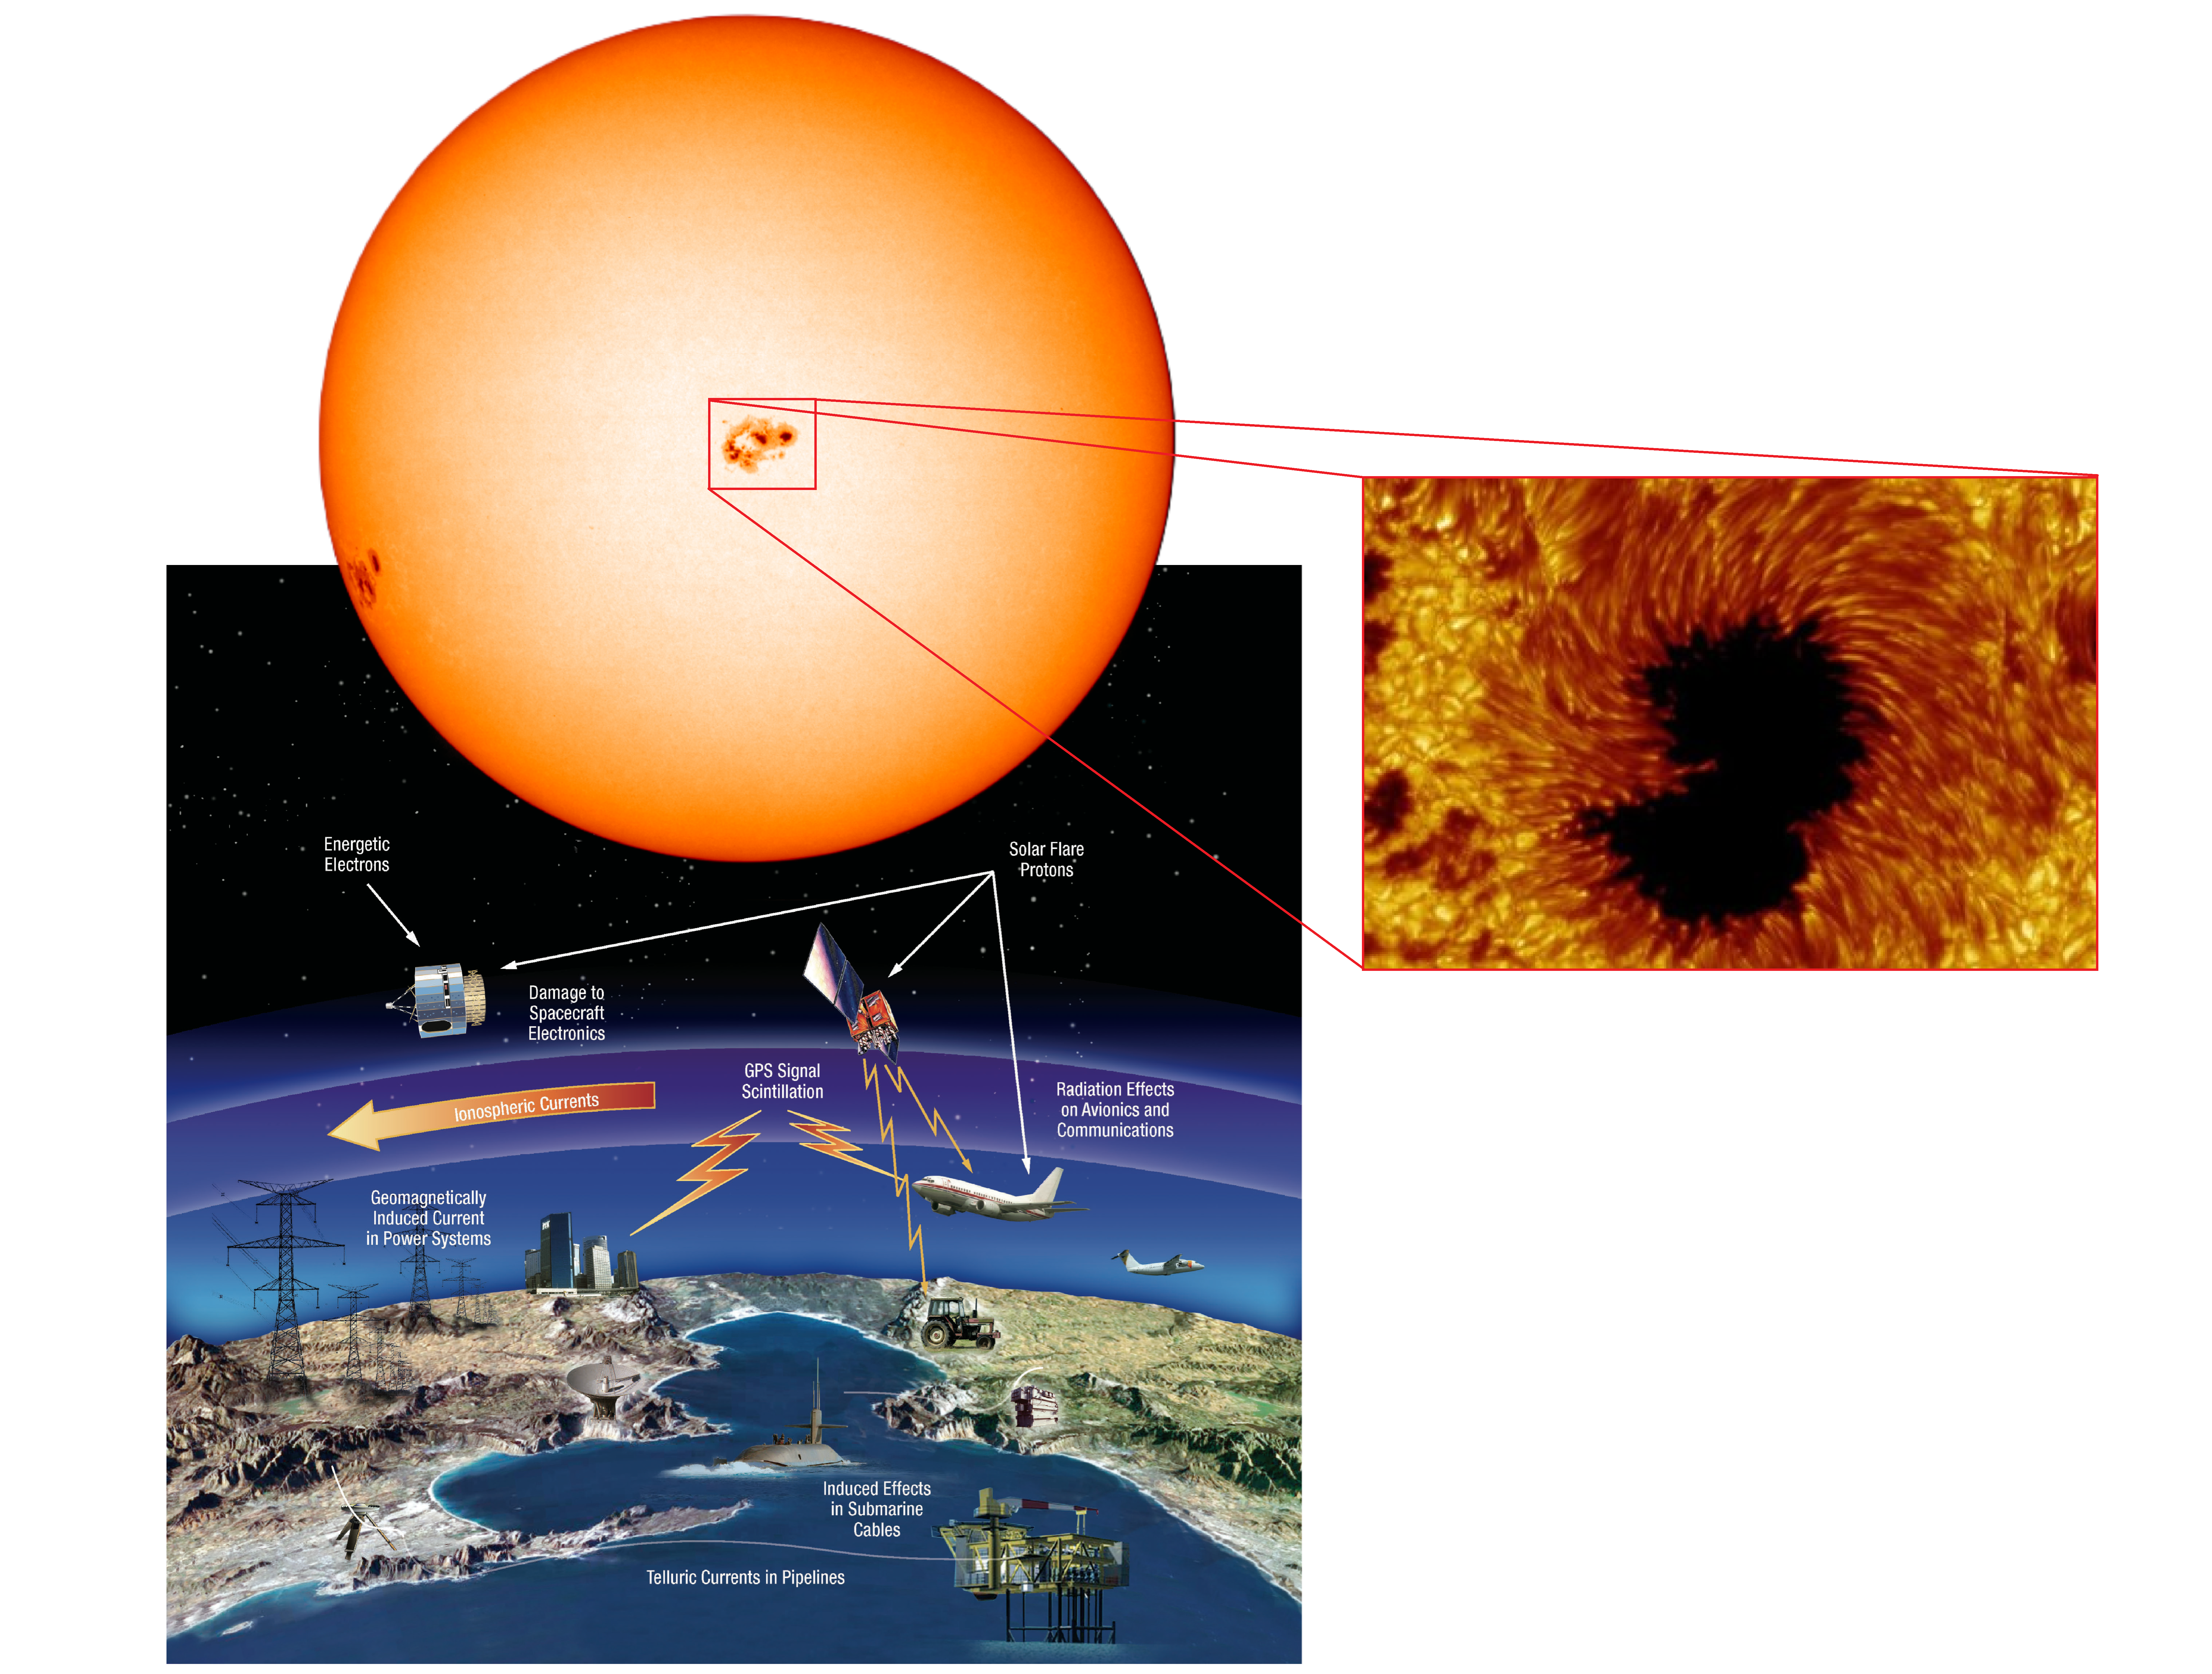
\includegraphics[height=0.8\textheight,width=\linewidth,keepaspectratio]{solar/space-weather-effects.png}\par
        \vspace{0.01cm}
        {\scriptsize Sistemas vulneráveis [1].}
        \column{0.49\textwidth}
        \centering
        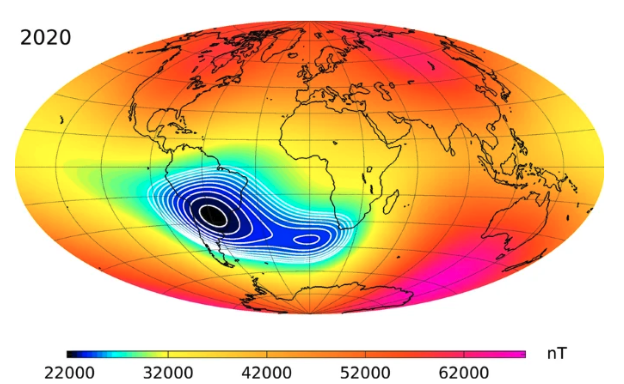
\includegraphics[height=0.6\textheight,width=\linewidth,keepaspectratio]{solar/south-atlantic-magnetic-anomaly-1.png}\par
        \vspace{0.01cm}
        {\scriptsize Anomalia magnética do Atlântico Sul [2].}
    \end{columns}
    
    \vfill
    {\raggedright\tiny\color{gray} [1] NASA Scientific Visualization Studio, “Solar Cycle Weather and Atmospheric Forcing Visualizations,” NASA Goddard Space Flight Center, v4.12, 2010.\par\vspace{0.03cm}
    [2] C. C. Finlay, C. Kloss, N. Olsen, M. D. Hammer, A. Grayver, y A. Kuvshinov, “The CHAOS-7 geomagnetic field model and observed changes in the South Atlantic Anomaly,” Earth, Planets and Space, vol. 72, art. no. 156, 2020.\par}
\end{frame}



% \begin{frame}{Manchas Solares}
%     \vspace{0.2cm} % Margen inicial sutil debajo del título del frame

%     \centering % Centra el bloque completo de columnas respecto al ancho de la diapositiva
%     \begin{columns}[c, onlytextwidth] % forces exact distribution across the text width
        
%         % Columna IZQUIERDA: Disco solar completo
%         \begin{column}{0.48\textwidth}
%             \centering
%             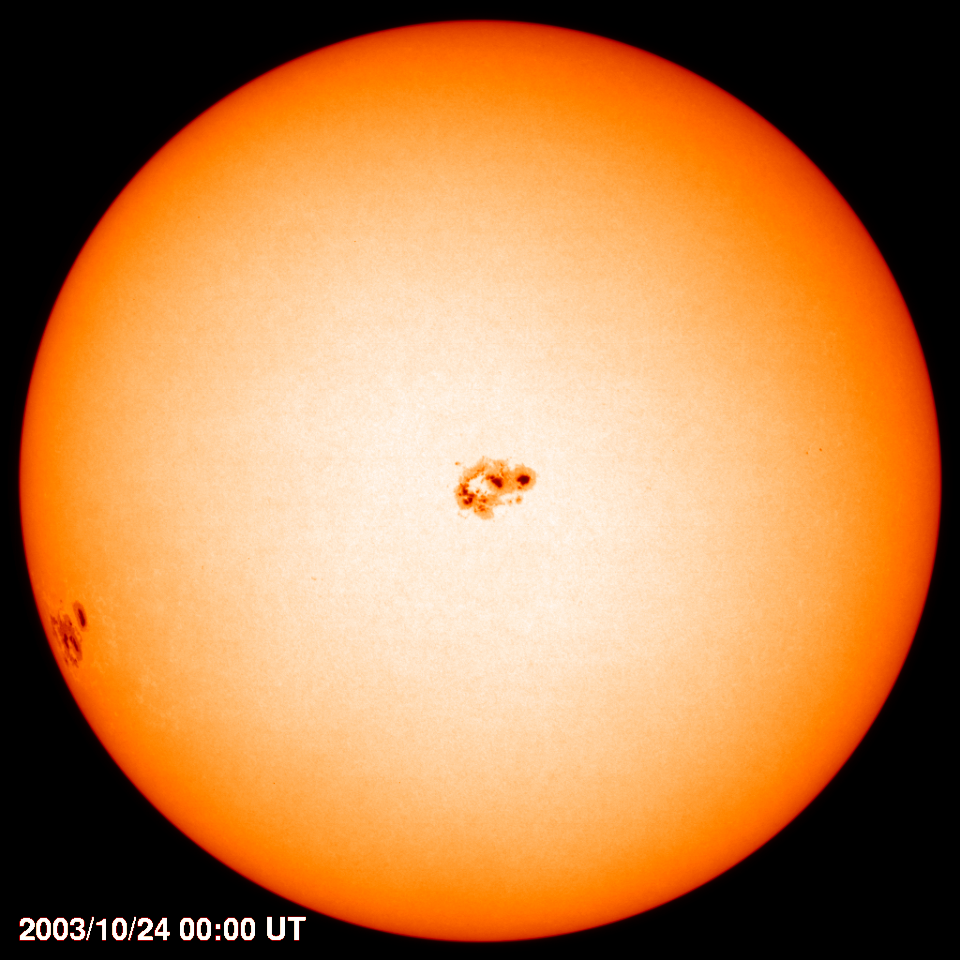
\includegraphics[height=0.55\textheight, width=\linewidth, keepaspectratio]{solar/sunspot.png}\par
%             \vspace{0.08cm}
%             {\scriptsize Disco solar completo [3].}
%         \end{column}
        
%         \hfill % Introduce un espacio elástico exacto en el medio para empujar las cosas a los extremos equilibrados
        
%         % Columna DERECHA: Detalle ampliado
%         \begin{column}{0.48\textwidth}
%             \centering
%             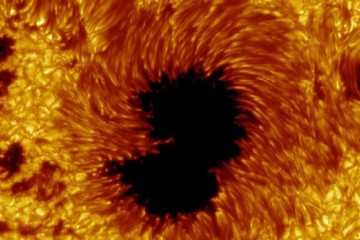
\includegraphics[height=0.55\textheight, width=\linewidth, keepaspectratio]{solar/spot_close.jpg}\par
%             \vspace{0.08cm}
%             {\scriptsize Detalle ampliado de una mancha solar [3].}
%         \end{column}
        
%     \end{columns}
    
%     \vfill % Empuja la referencia estrictamente al límite inferior de la diapositiva

%     % Bloque de Referencia a pie de página
%     {\tiny\color{gray} [3] P. H. Scherrer et al., “The Helioseismic and Magnetic Imager (HMI) investigation on the Solar Dynamics Observatory (SDO),” \textit{Solar Physics}, vol. 275, pp. 207--227, 2012.}
% \end{frame}


% \begin{frame}{Introducción: Efectos del clima espacial}
%     \centering
%     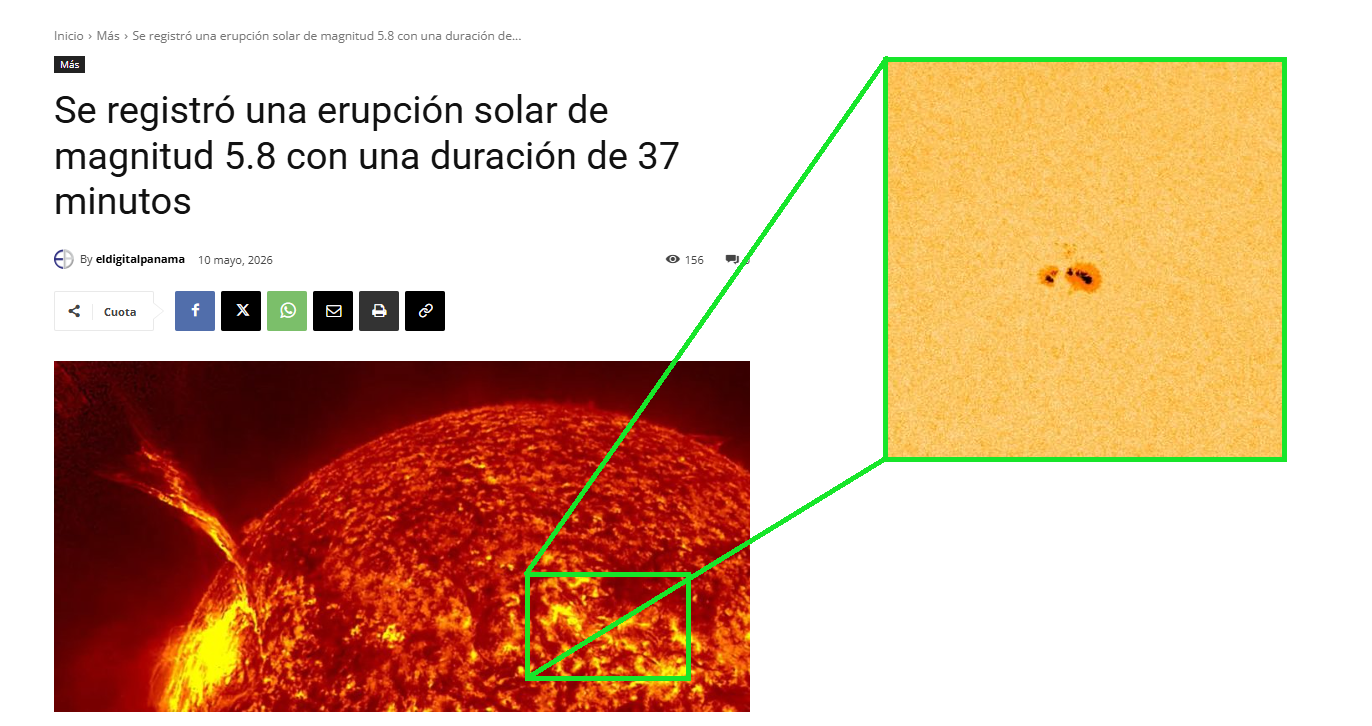
\includegraphics[height=0.65\textheight,width=0.96\linewidth,keepaspectratio]{solar/news.png}

%     \vspace{0.05cm}

%     \vfill
%     \begin{minipage}{0.95\linewidth}
%         \centering\small
%         El Instituto de Geofísica Aplicada de Rusia comunicó que el 10 de mayo se registró una erupción solar de magnitud 5.8 de 37 minutos proveniente del grupo de manchas solares 4436.
%     \end{minipage}\par
% \end{frame}



% \begin{frame}{Introducción: Clima espacial y sistemas tecnológicos}
%     \centering
%     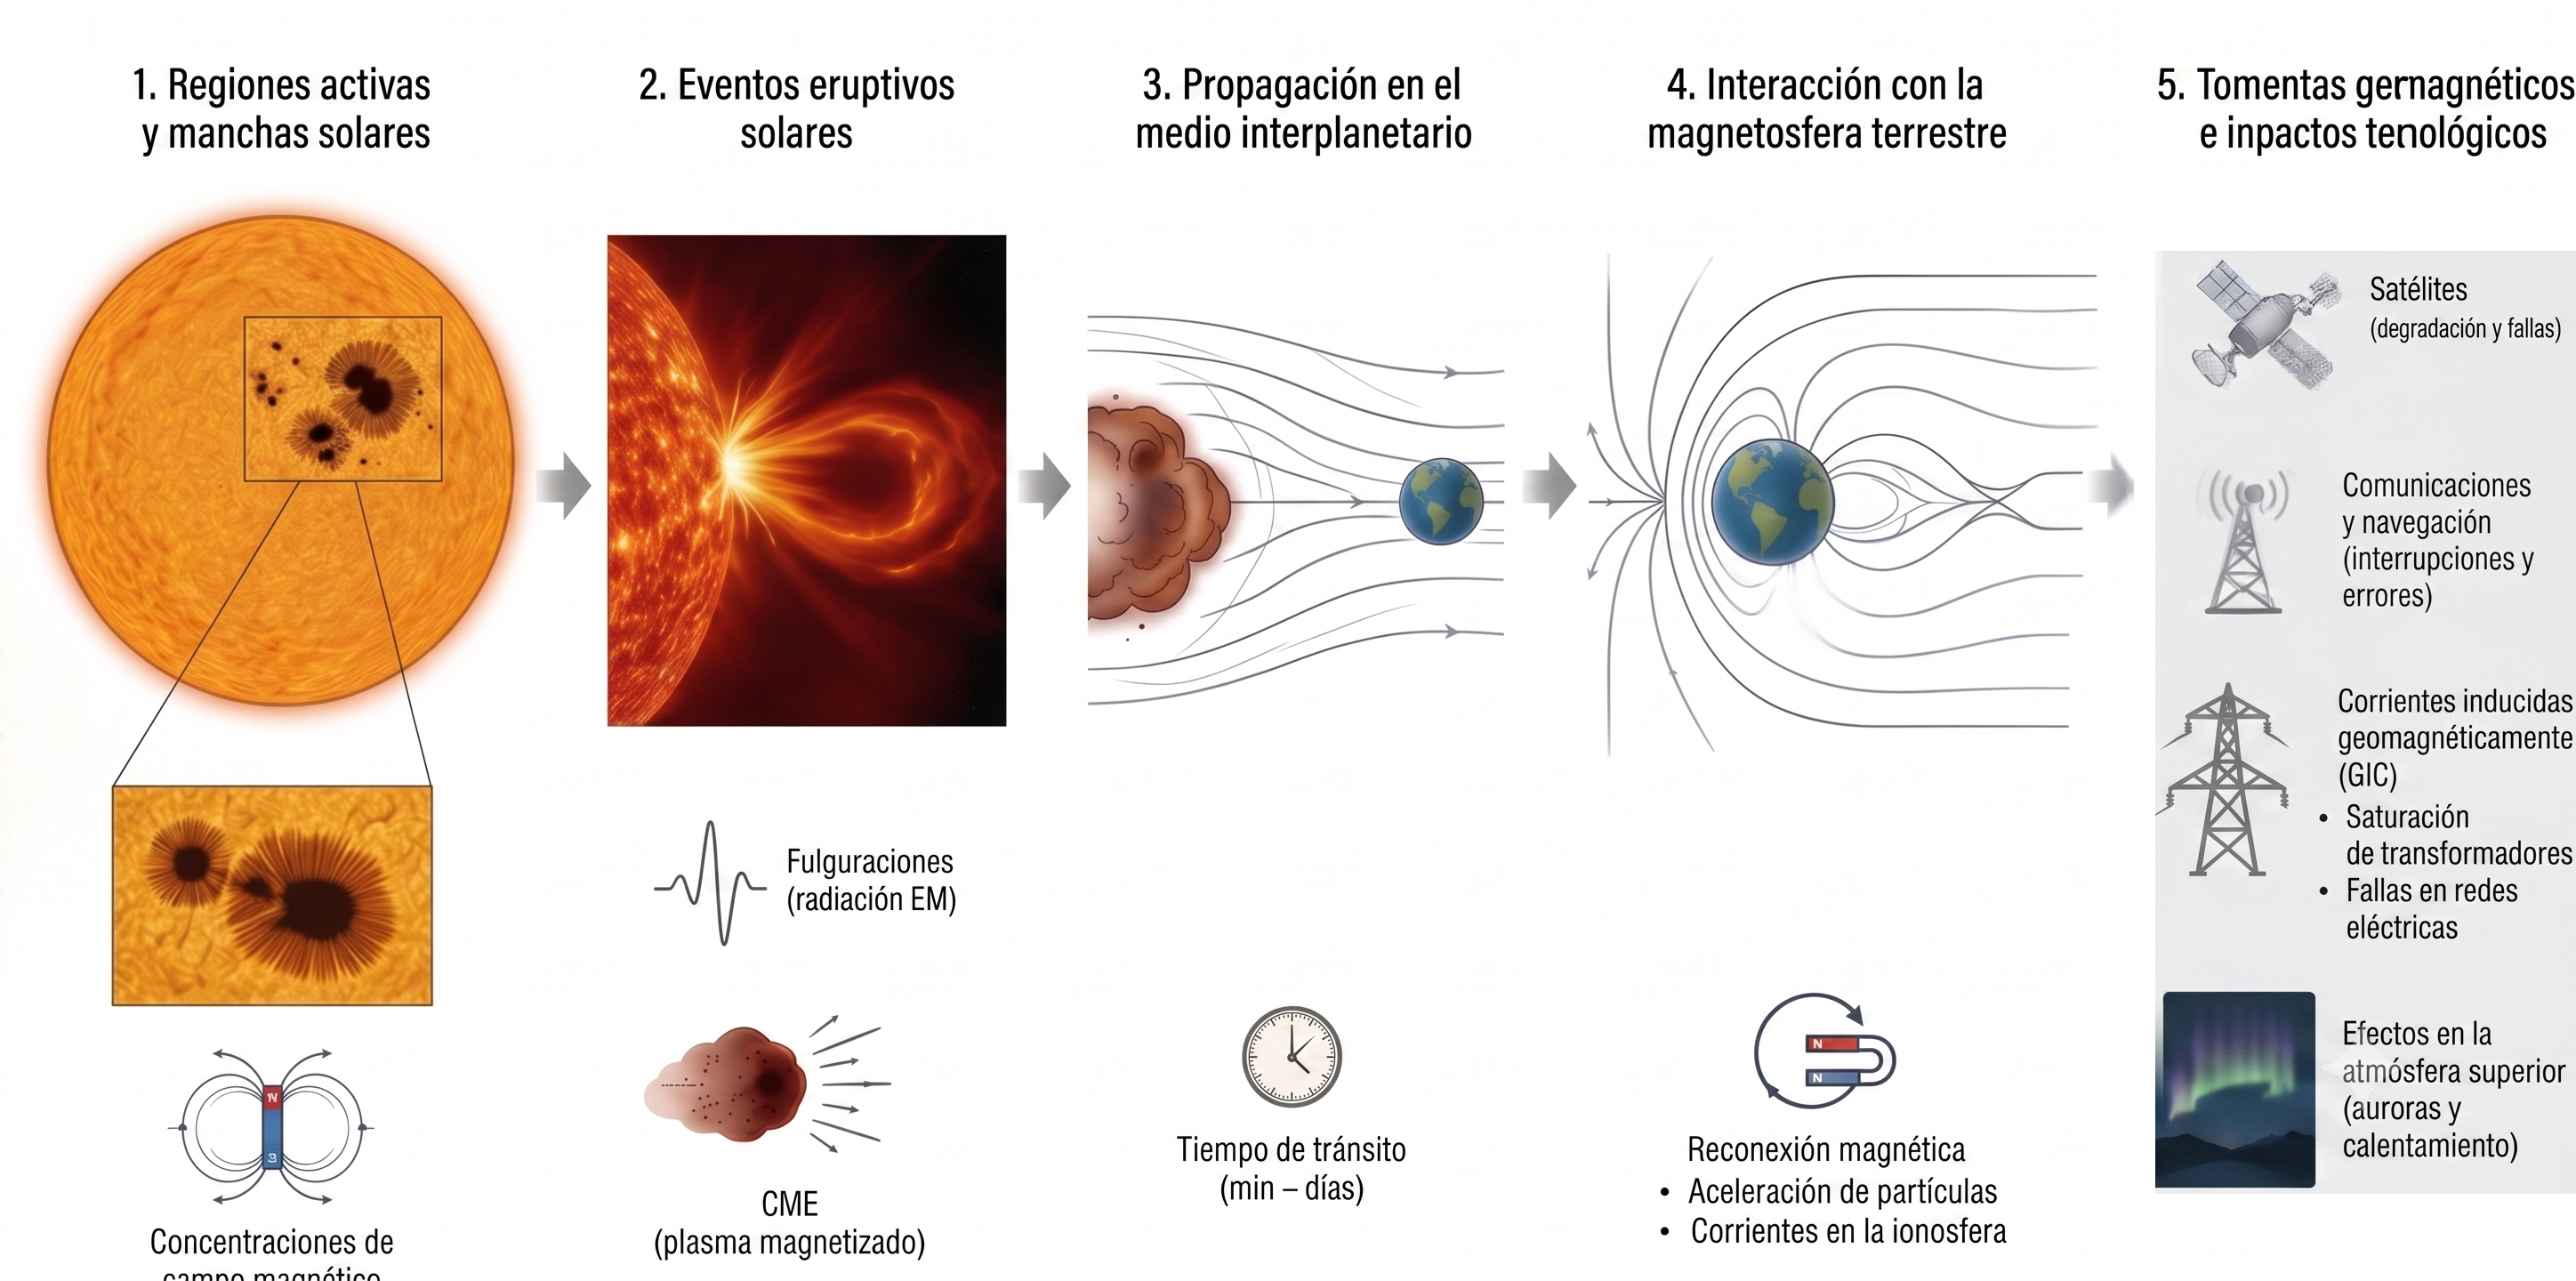
\includegraphics[height=0.65\textheight,width=0.96\linewidth,keepaspectratio]{solar/cycle_solar.png}\par
%     \vspace{0.05cm}
%     %{\footnotesize Adaptado de Hathaway [2]}\par
    
%     \vfill
%     \begin{minipage}{0.95\linewidth}
%         \centering\small
%         Manchas solares: evolución fotosférica. Clima espacial: telecomunicaciones, electrónica y redes. Flujo local: observar, registrar, clasificar, predecir.
%     \end{minipage}\par
    
%     \vspace{0.1cm}
%     %{\tiny\color{gray} [2] D. H. Hathaway, “The solar cycle,” Living Reviews in Solar Physics, vol. 12, no. 1, pp. 1--70, 2015.\par}
% \end{frame}

% \begin{frame}{Introducción: Contexto Nacional}
%     \centering
%     \vfill
%     \begin{minipage}{0.75\linewidth}
%         \centering
%         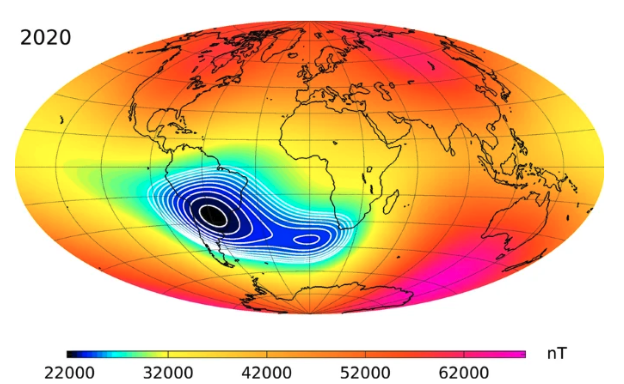
\includegraphics[height=0.66\textheight,keepaspectratio]{solar/south-atlantic-magnetic-anomaly-1.png}\par
%         \vspace{0.1cm}
%         {\footnotesize Anomalía magnética del Atlántico Sur [2]}
%     \end{minipage}\par
    
%     \vfill
%     {\tiny\color{gray} [2] C. C. Finlay, C. Kloss, N. Olsen, M. D. Hammer, A. Grayver, y A. Kuvshinov, “The CHAOS-7 geomagnetic field model and observed changes in the South Atlantic Anomaly,” Earth, Planets and Space, vol. 72, art. no. 156, 2020.\par}
% \end{frame}

\begin{frame}{Introdução: Monitoramento local de manchas solares}
    \centering
    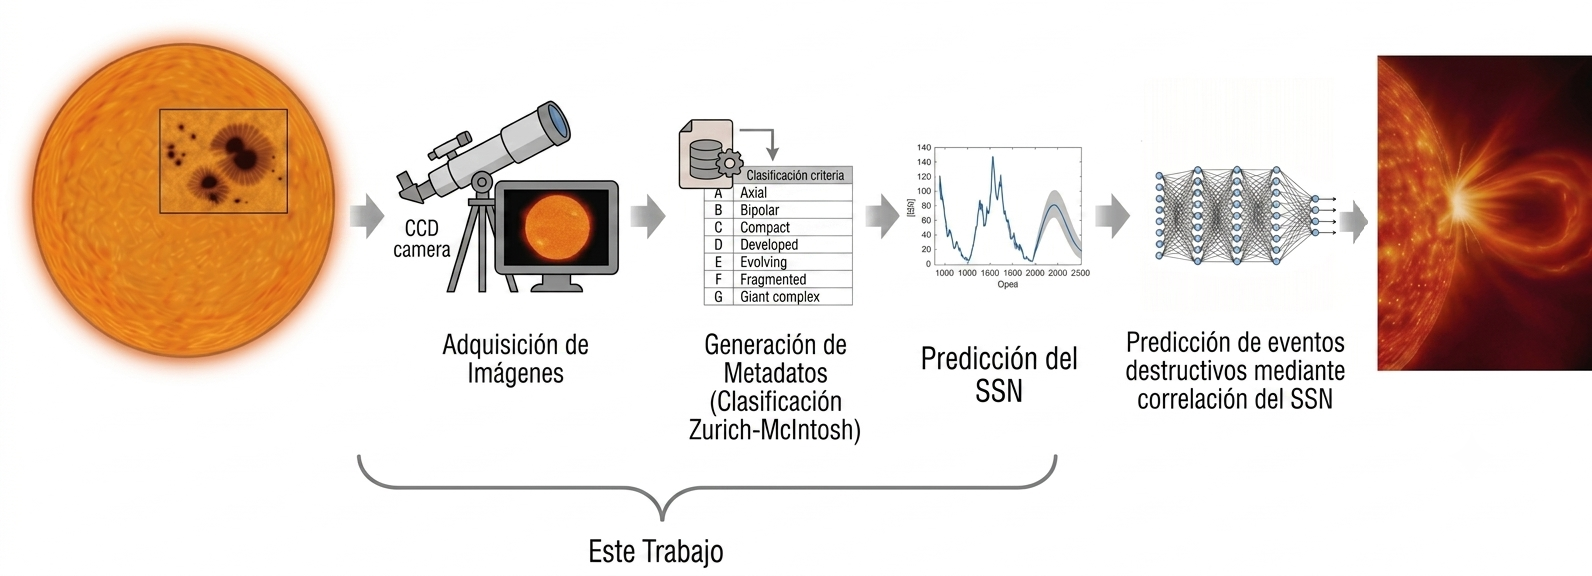
\includegraphics[height=0.65\textheight,width=0.96\linewidth,keepaspectratio]{solar/monitoreo.png}

    \vspace{0.05cm}

    \vfill
    \begin{minipage}{0.95\linewidth}
        \centering\small
        Fluxo de trabalho deste projeto.
    \end{minipage}\par
    
\end{frame}

% \begin{frame}{Introducción: Alcance}
%     \small
%     \vspace{-0.2cm}

%     % BLOQUE SUPERIOR: Problemáticas de la Introducción
%     \begin{block}{Problemáticas Identificadas}
%         \scriptsize
%         \begin{itemize}
%             \item \textbf{Desafío en Clasificación:} Alta complejidad semántica y estructural en las manchas solares.
%             \item \textbf{Vacío Tecnológico:} Ausencia de un ecosistema completo y local de adquisición y registro.
%             \item \textbf{Carencia de Datos:} Falta de una base de datos etiquetada bajo estándares internacionales.
%         \end{itemize}
%     \end{block}

%     \vspace{0.1cm}

%     % BLOQUE INFERIOR: Respuestas / Contribuciones del trabajo
%     \begin{block}{Contribuciones del Trabajo (Soluciones Desarrolladas)}
%         \scriptsize
%         \begin{enumerate}
%             \item \contrib{Dispositivo de Adquisición:} Hardware local para captura solar.
%             \item \contrib{Base de Datos Etiquetada:} Repositorio estructurado para el entrenamiento de modelos.
%             \item \contrib{Modelo DMD--Spörer:} Análisis predictivo de la distribución latitudinal.
%             \item \contrib{Clasificador Jerárquico de Deep Learnign:} Clasificador taxonómico Zurich-McIntosh.
%             \item \contrib{Plataforma de Observación:} Sistema integrado híbrido para asistencia en tiempo real.
%         \end{enumerate}
%     \end{block}
% \end{frame}


\begin{frame}{Objetivos do Trabalho}
    \begin{block}{Objetivo Geral}
        \scriptsize
        Desenvolver um protótipo para a detecção e classificação local de manchas solares, integrando técnicas de visão computacional, inteligência artificial e análise preditiva da atividade solar para observatórios locais.
    \end{block}

    \vspace{0.1cm}
    \begin{block}{Objetivos Específicos}
        \scriptsize
        \begin{enumerate}
            \item Analisar registros históricos de manchas solares a partir de imagens heliográficas.
            \item Projetar um fluxo de aquisição e pré-processamento de imagens para vincular observações locais a relatórios internacionais.
            \item Desenvolver um detector de grupos solares e um classificador hierárquico de caracteres Zürich--McIntosh preservando dependências semânticas.
            \item Implementar um módulo preditivo da evolução temporal e distribuição latitudinal de manchas solares a partir de registros históricos.
            \item Validar o funcionamento integral do protótipo em ambiente de observação.
        \end{enumerate}
    \end{block}
\end{frame}

\section{Fundamentação Teórica}

% \begin{frame}{Modalidades de Observación Solar}
%     \centering
    
%     \begin{columns}
%         \column{0.49\textwidth}
%         \centering
%         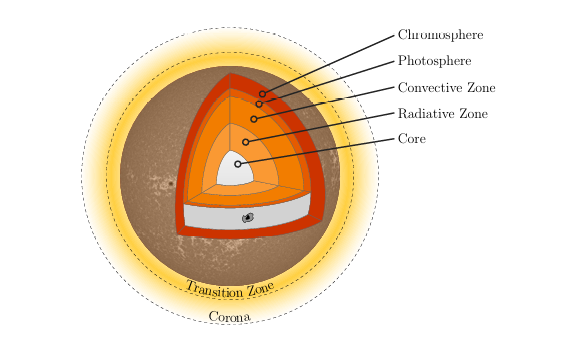
\includegraphics[height=0.6\textheight,width=\linewidth,keepaspectratio]{solar/sun_parts.png}\par
%         \vspace{0.05cm}
%         {\scriptsize Capas y regiones del Sol [4].}
%         \column{0.49\textwidth}
%         \centering
%         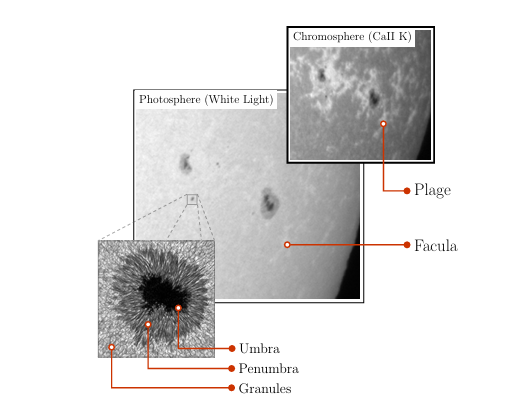
\includegraphics[height=0.6\textheight,width=\linewidth,keepaspectratio]{solar/wl_cak.png}\par
%         \vspace{0.05cm}
%         {\scriptsize Comparación luz blanca y CaII K [4].}
%     \end{columns}
    
%     \vfill
%     {\tiny\color{gray} [4] M. Sayez et al., “SunSCC: Automated solar classification dataset” Astronomy \& Astrophysics, 2023.}
% \end{frame}

% \begin{frame}{Manchas Solares}
%     \vspace{0.2cm} % Margen inicial sutil debajo del título del frame

%     \centering % Centra el bloque completo de columnas respecto al ancho de la diapositiva
%     \begin{columns}[c, onlytextwidth] % forces exact distribution across the text width
        
%         % Columna IZQUIERDA: Disco solar completo
%         \begin{column}{0.48\textwidth}
%             \centering
%             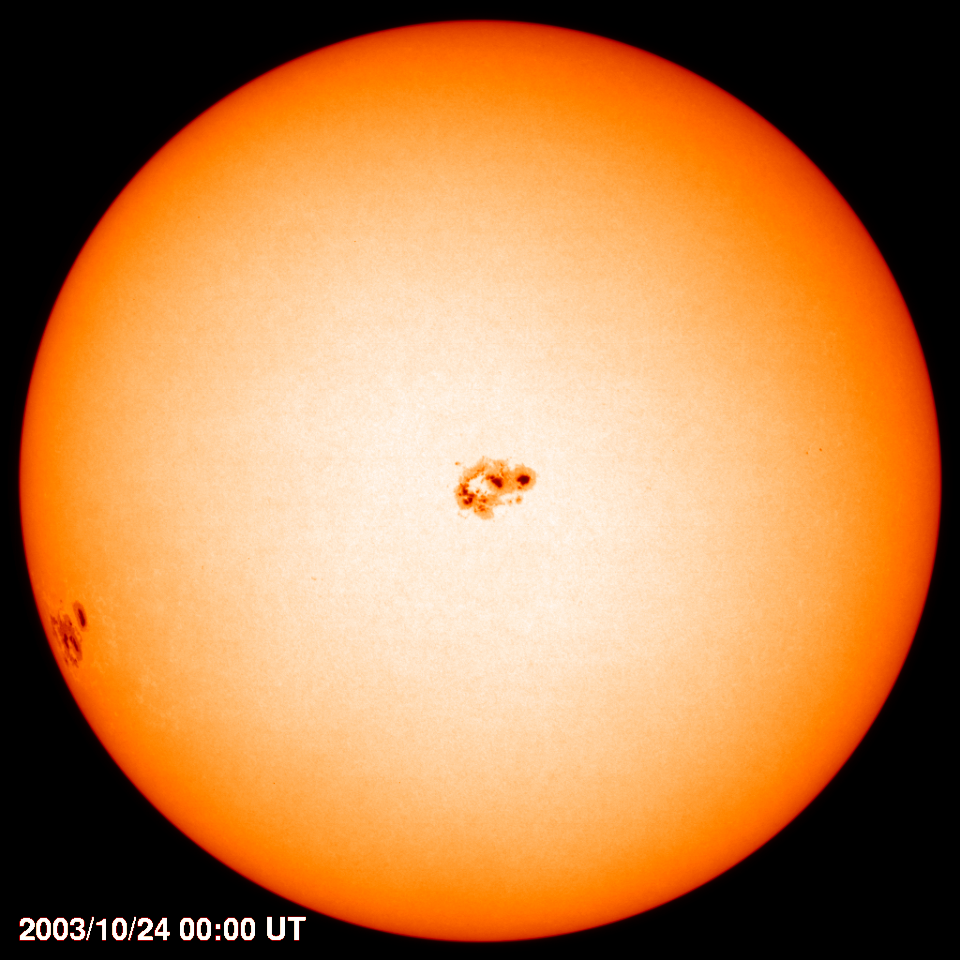
\includegraphics[height=0.55\textheight, width=\linewidth, keepaspectratio]{solar/sunspot.png}\par
%             \vspace{0.08cm}
%             {\scriptsize Disco solar completo [3].}
%         \end{column}
        
%         \hfill % Introduce un espacio elástico exacto en el medio para empujar las cosas a los extremos equilibrados
        
%         % Columna DERECHA: Detalle ampliado
%         \begin{column}{0.48\textwidth}
%             \centering
%             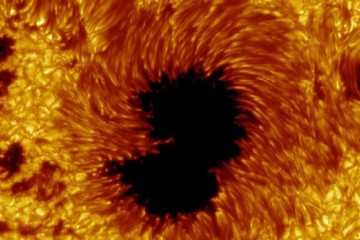
\includegraphics[height=0.55\textheight, width=\linewidth, keepaspectratio]{solar/spot_close.jpg}\par
%             \vspace{0.08cm}
%             {\scriptsize Detalle ampliado de una mancha solar [3].}
%         \end{column}
        
%     \end{columns}
    
%     \vfill % Empuja la referencia estrictamente al límite inferior de la diapositiva

%     % Bloque de Referencia a pie de página
%     {\tiny\color{gray} [3] P. H. Scherrer et al., “The Helioseismic and Magnetic Imager (HMI) investigation on the Solar Dynamics Observatory (SDO),” \textit{Solar Physics}, vol. 275, pp. 207--227, 2012.}
% \end{frame}

\begin{frame}{Sistemas de Classificação de Manchas Solares}
    \begin{columns}
        \column{0.49\textwidth}
        \centering
        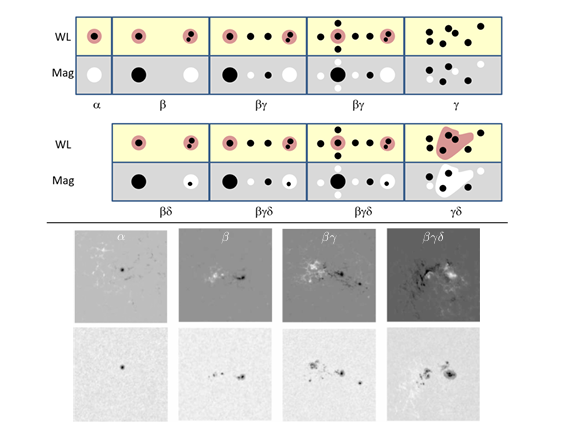
\includegraphics[height=0.6\textheight,width=\linewidth,keepaspectratio]{solar/wilson.png}\par
        \vspace{0.05cm}
        {\scriptsize Classificação de Wilson (8 classes) [3].}
        \column{0.49\textwidth}
        \centering
        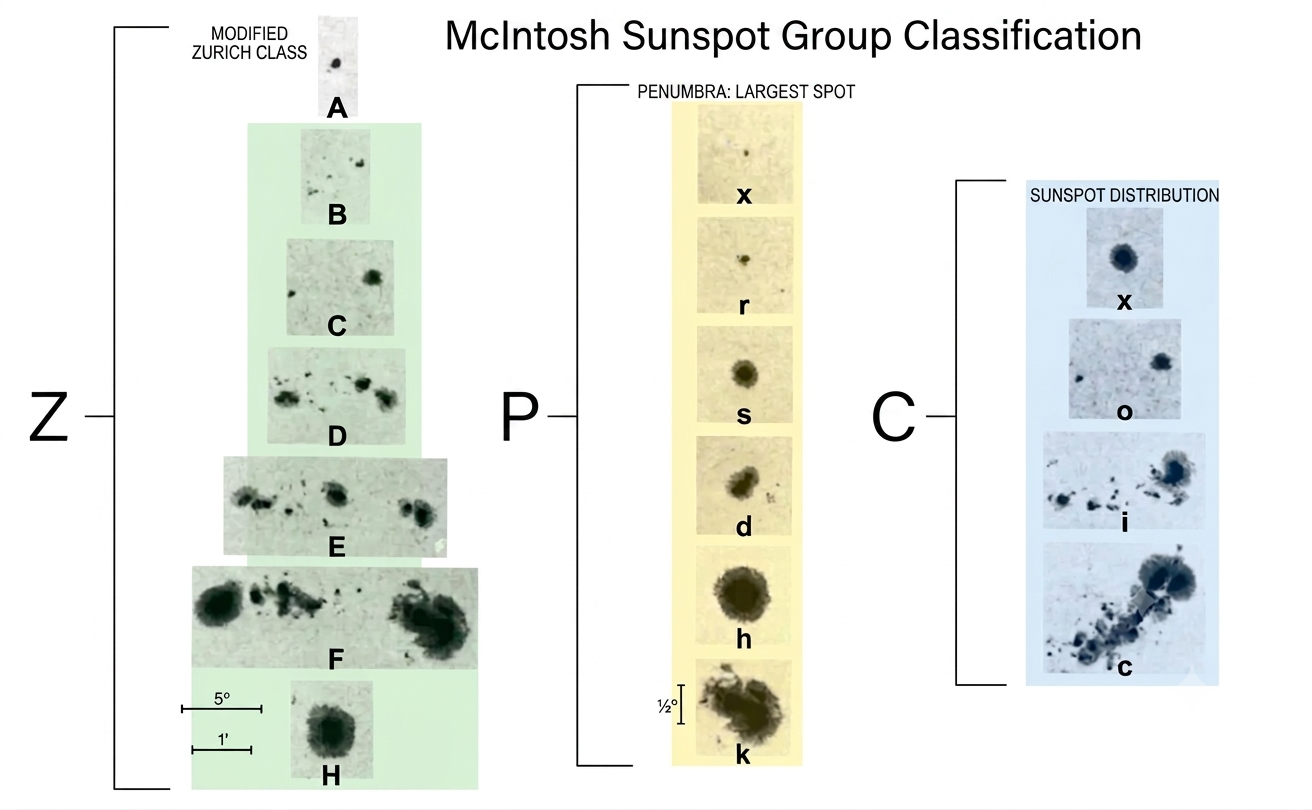
\includegraphics[height=0.6\textheight,width=\linewidth,keepaspectratio]{solar/mcintosh.png}\par
        \vspace{0.05cm}
        {\scriptsize Classificação de Zürich--McIntosh (60 classes) [3].}
    \end{columns}\par
    
    \vfill
    {\raggedright\tiny\color{gray} [3] P. S. McIntosh, “The classification of sunspot groups,” Solar Physics, vol. 125, no. 2, pp. 251--267, 1990.\par}
\end{frame}

\begin{frame}{Ciclo Solar}
    \centering
    \vspace{0.05cm}
    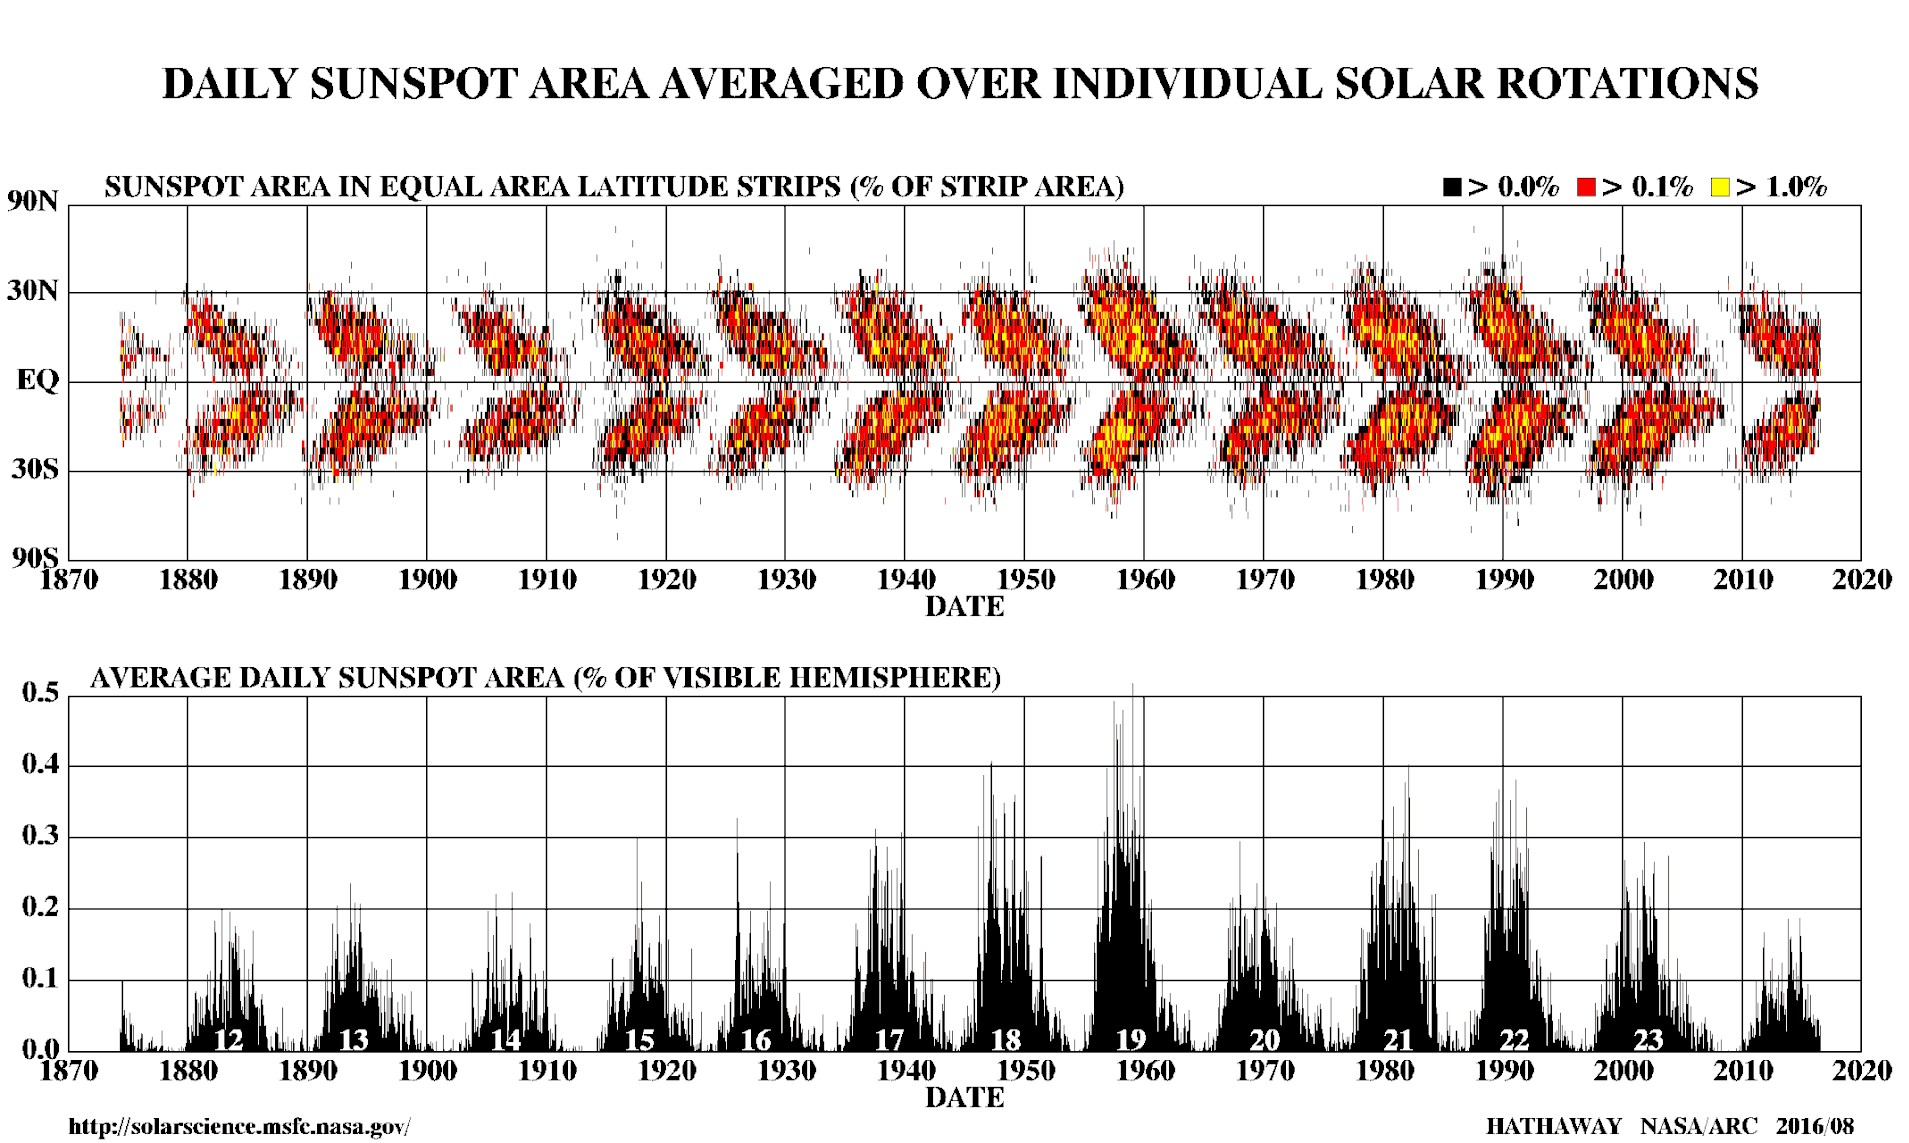
\includegraphics[width=\linewidth, height=0.68\textheight, keepaspectratio]{solar/butterfly.jpg}\par
    \vspace{0.04cm}
    {\scriptsize Diagrama de Spörer histórico [4].}\par
    
    \vfill
    {\raggedright\tiny\color{gray} [4] D. H. Hathaway, “The solar cycle,” Living Reviews in Solar Physics, vol. 12, no. 1, pp. 1--70, 2015.\par}
\end{frame}

% \begin{frame}{Observatorios Terrestres y Contexto Local}
%     \centering
%     \begin{columns}
%         \column{0.32\textwidth}
%         \centering
%         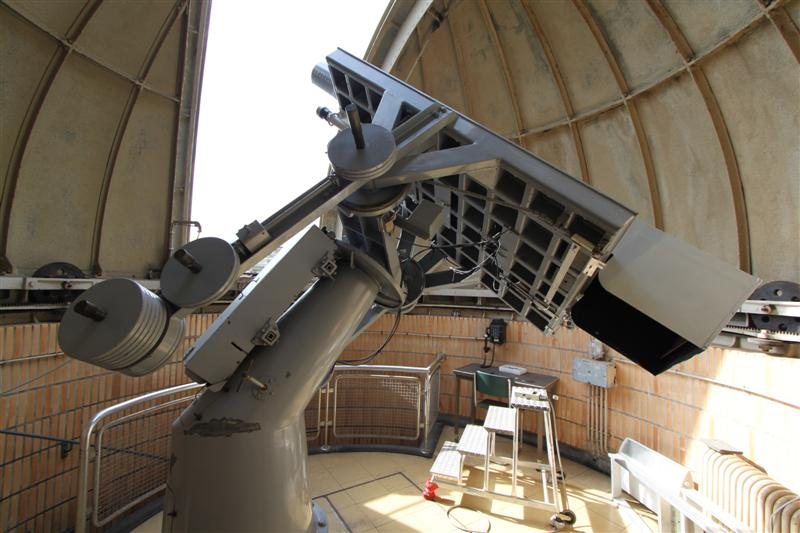
\includegraphics[height=0.46\textheight,width=\linewidth,keepaspectratio]{solar/scope_proj.jpg}\par
%         \vspace{0.05cm}
%         {\scriptsize Plataforma USET [6].}
%         \column{0.32\textwidth}
%         \centering
%         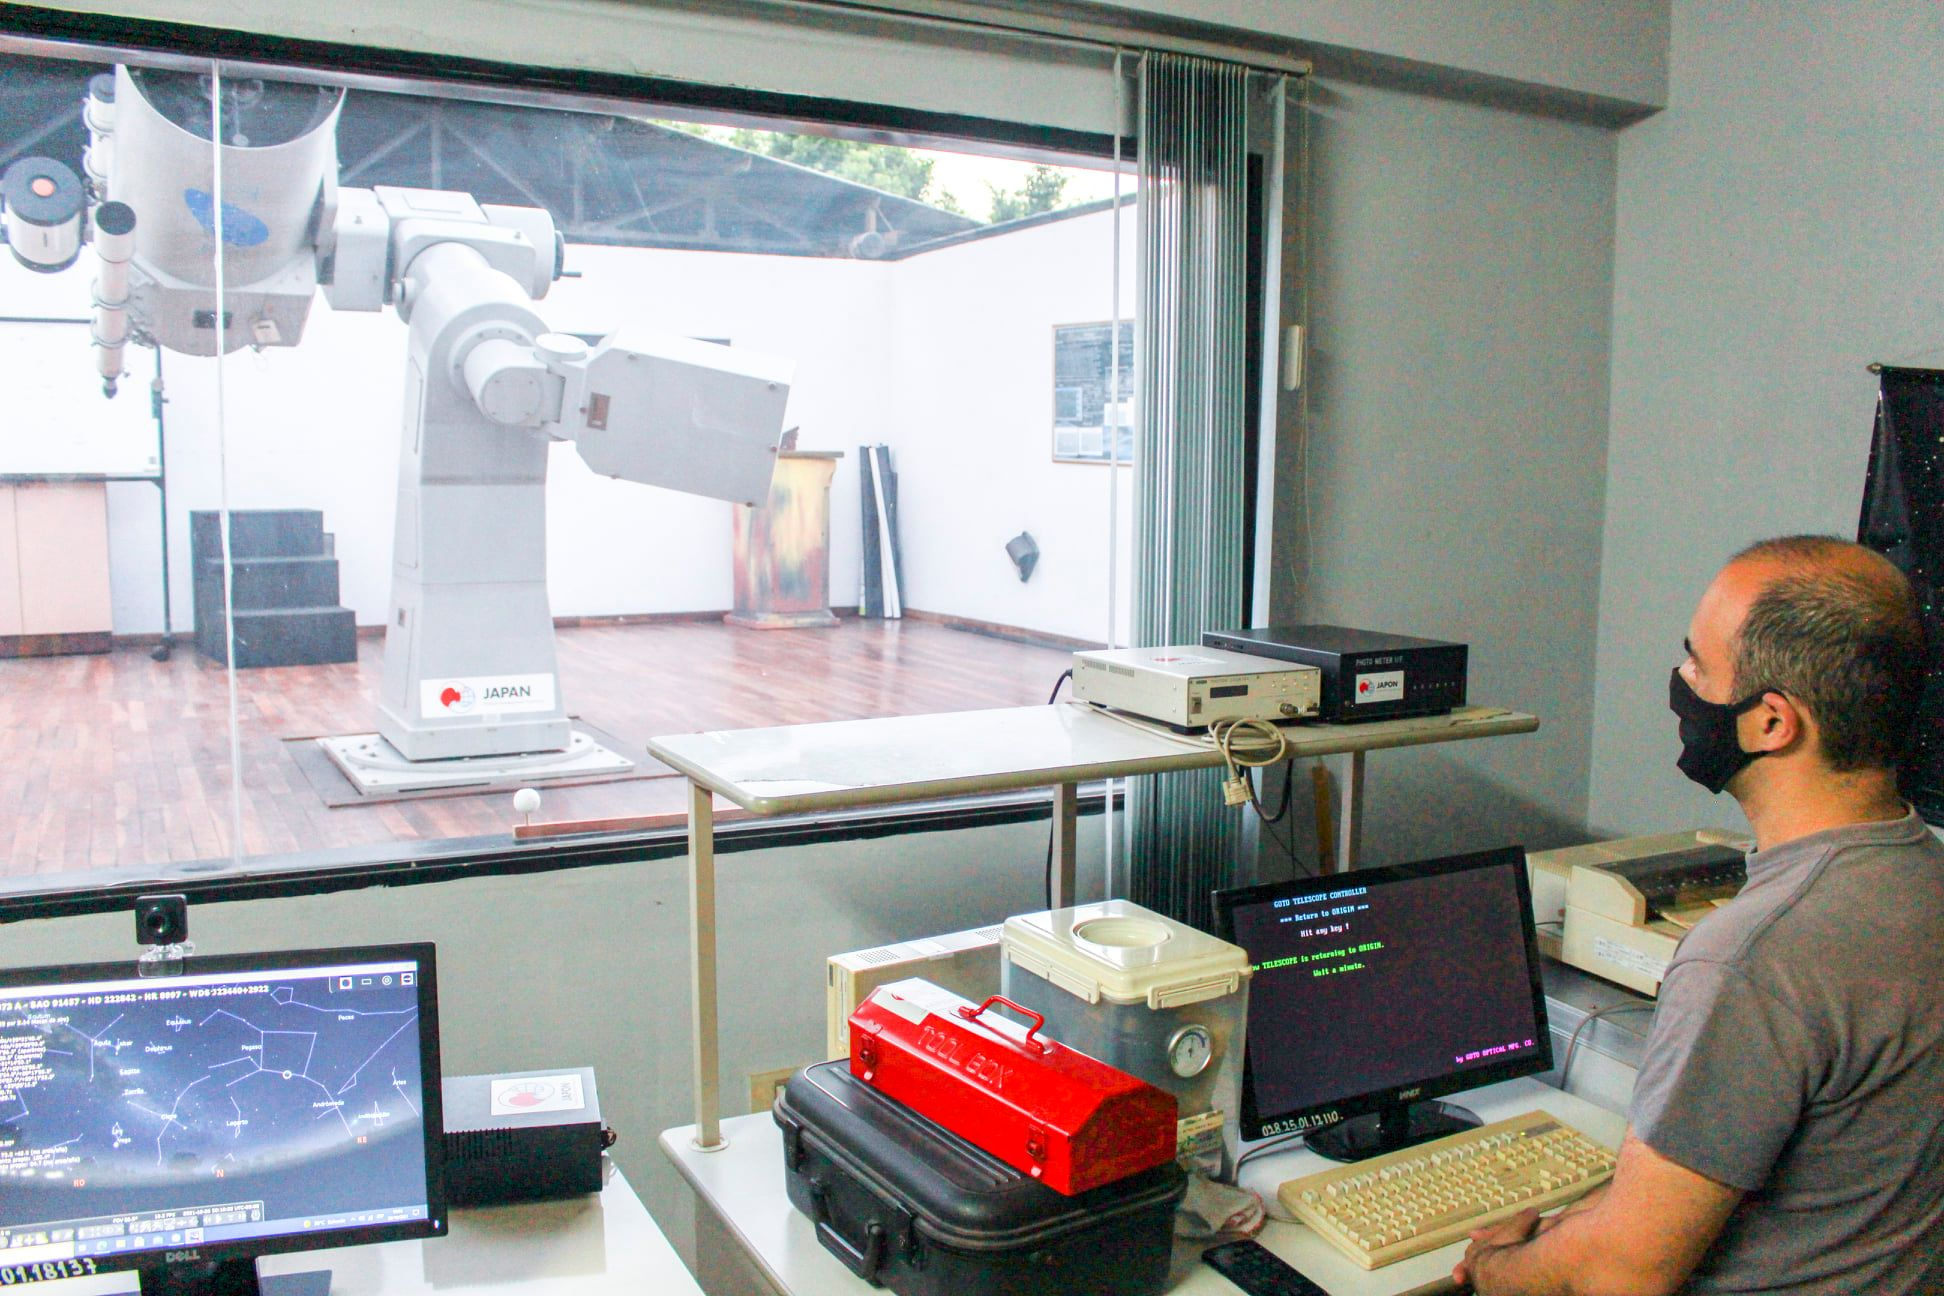
\includegraphics[height=0.46\textheight,width=\linewidth,keepaspectratio]{obs/control.jpg}\par
%         \vspace{0.05cm}
%         {\scriptsize Sala de control del observatorio "Prof. Alexis Troche Boggino".}
%         \column{0.32\textwidth}
%         \centering
%         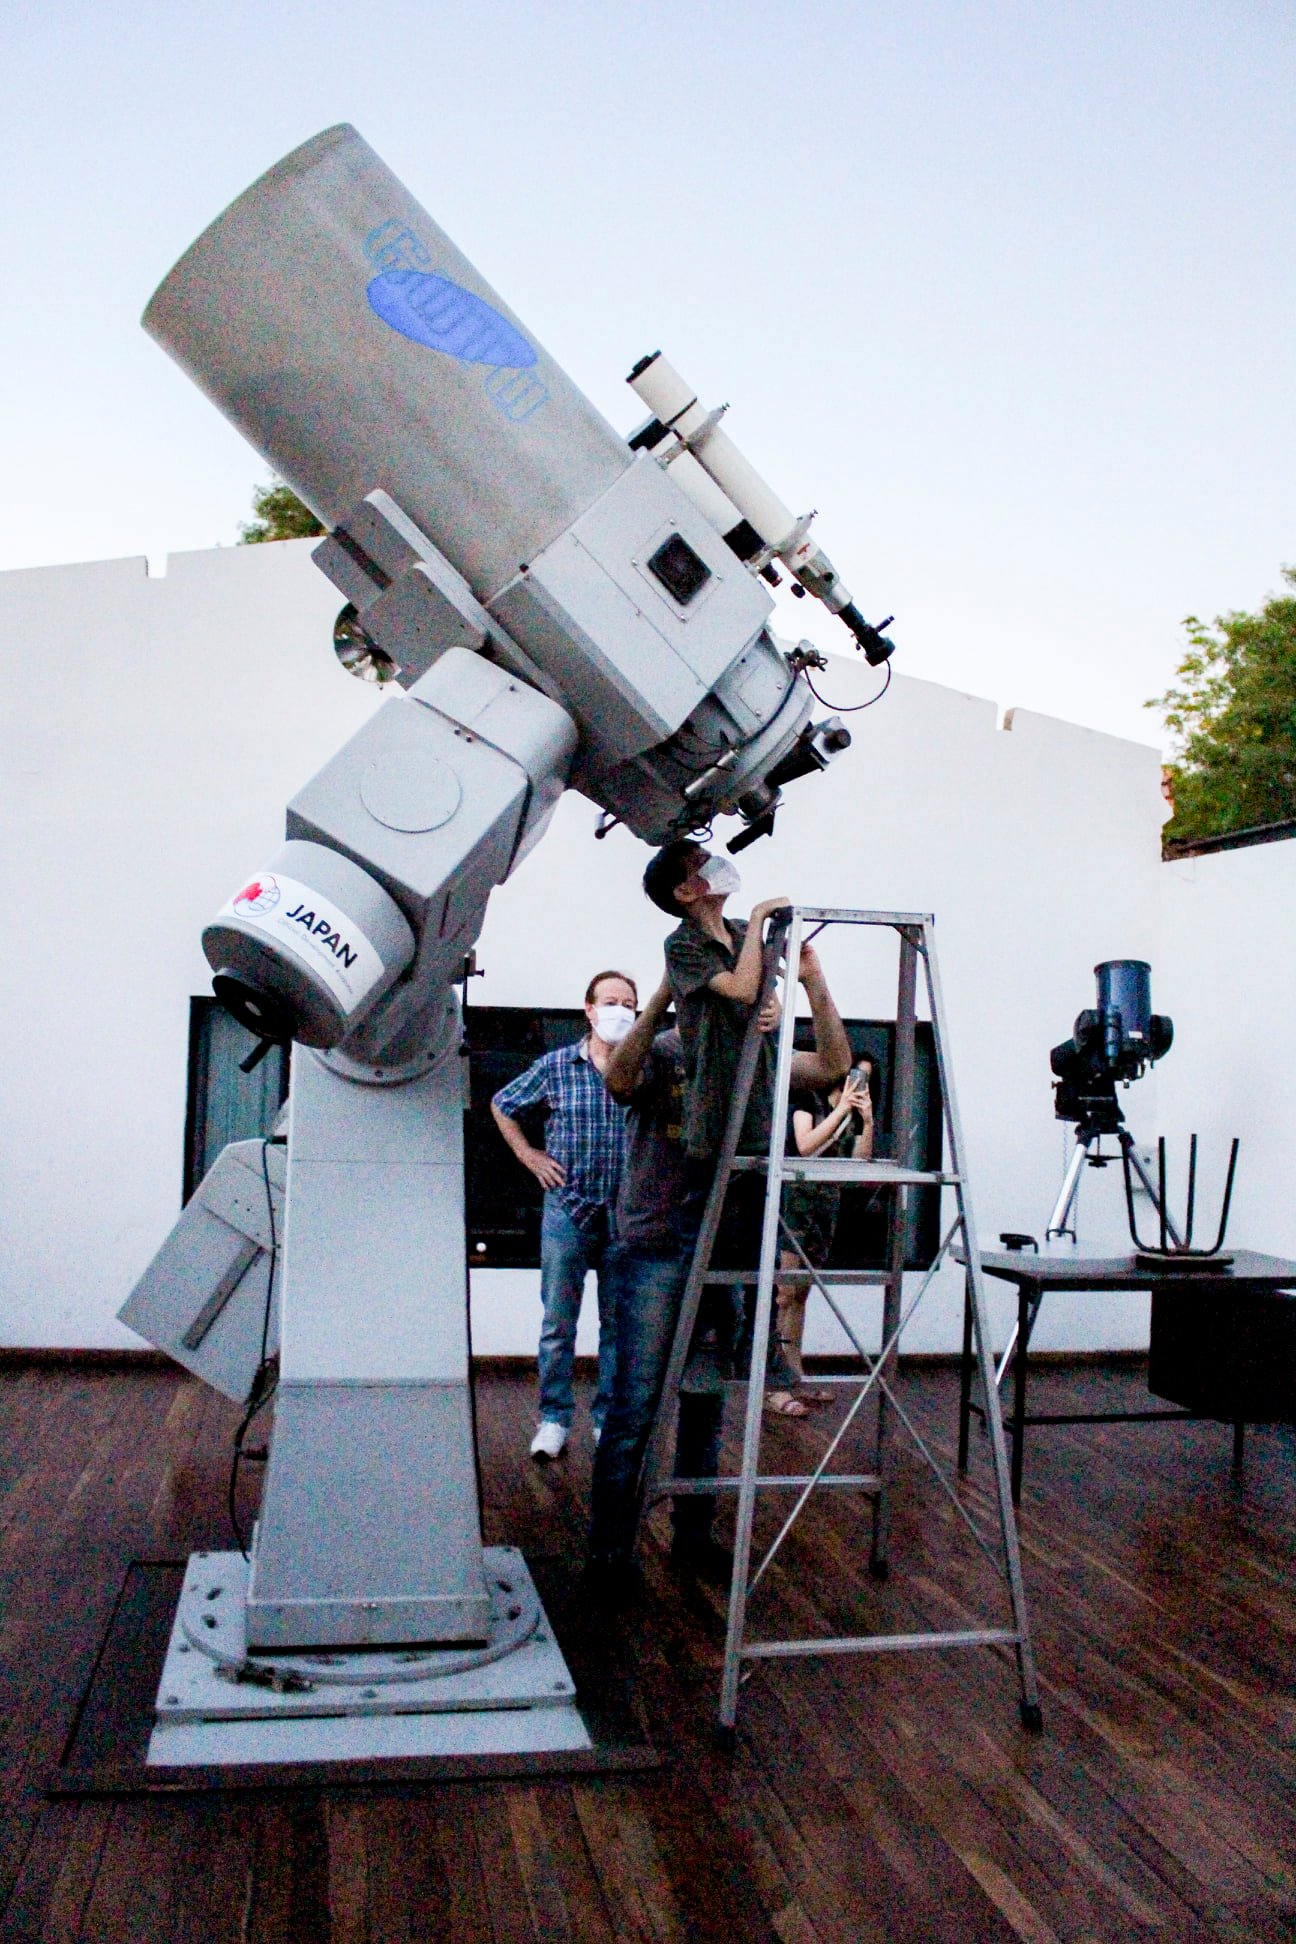
\includegraphics[height=0.46\textheight,width=\linewidth,keepaspectratio]{obs/scope.jpg}\par
%         \vspace{0.05cm}
%         {\scriptsize Telescopio del Observatorio "Prof. Alexis Troche Boggino".}
%     \end{columns}
    
%     \vfill
%     {\tiny\color{gray} [6] Royal Observatory of Belgium, “Understanding Solar Activity Telescopes (USET) report,” 2026.}
% \end{frame}


% \section{Estado del Arte}

% \begin{frame}{Estado del Arte: Contexto y Brecha Tecnológica}
%     \begin{block}{La Brecha en el Mercado Actual}
%         En la actualidad, \textbf{no existen ecosistemas comerciales} de observación astrofotográfica que integren de extremo a extremo todo el flujo de trabajo científico:
%     \end{block}

%     \vspace{0.3cm}
%     \begin{columns}[T]
%         \column{0.45\textwidth}
%         \centering
%         \textbf{Flujo Comercial Convencional}
%         \vspace{0.2cm}
%         \begin{itemize}
%             \item Adquisición asistida aislada.
%             \item Dependencia de software de terceros.
%             \item Sin análisis científico local.
%         \end{itemize}

%         \column{0.10\textwidth}
%         \centering
%         \vspace{0.6cm}
%         $\mathbf{\Longrightarrow}$

%         \column{0.45\textwidth}
%         \centering
%         \textbf{Propuesta del Prototipo}
%         \vspace{0.2cm}
%         \begin{itemize}
%             \item \color{deepblue} Captura + Preprocesamiento local.
%             \item \color{deepblue} Inferencia por IA en cascada.
%             \item \color{deepblue} Modelos predictivos del ciclo solar.
%         \end{itemize}
%     \end{columns}

%     \vspace{0.4cm}
%     \centering
%     \small \textit{Por lo tanto, el estado del arte se analiza bajo las siguientes dimensiones críticas:}
% \end{frame}

% \begin{frame}{Dispositivos comerciales de adquisición asistida}
%     \begin{columns}
%         \column{0.32\textwidth}
%         \centering
%         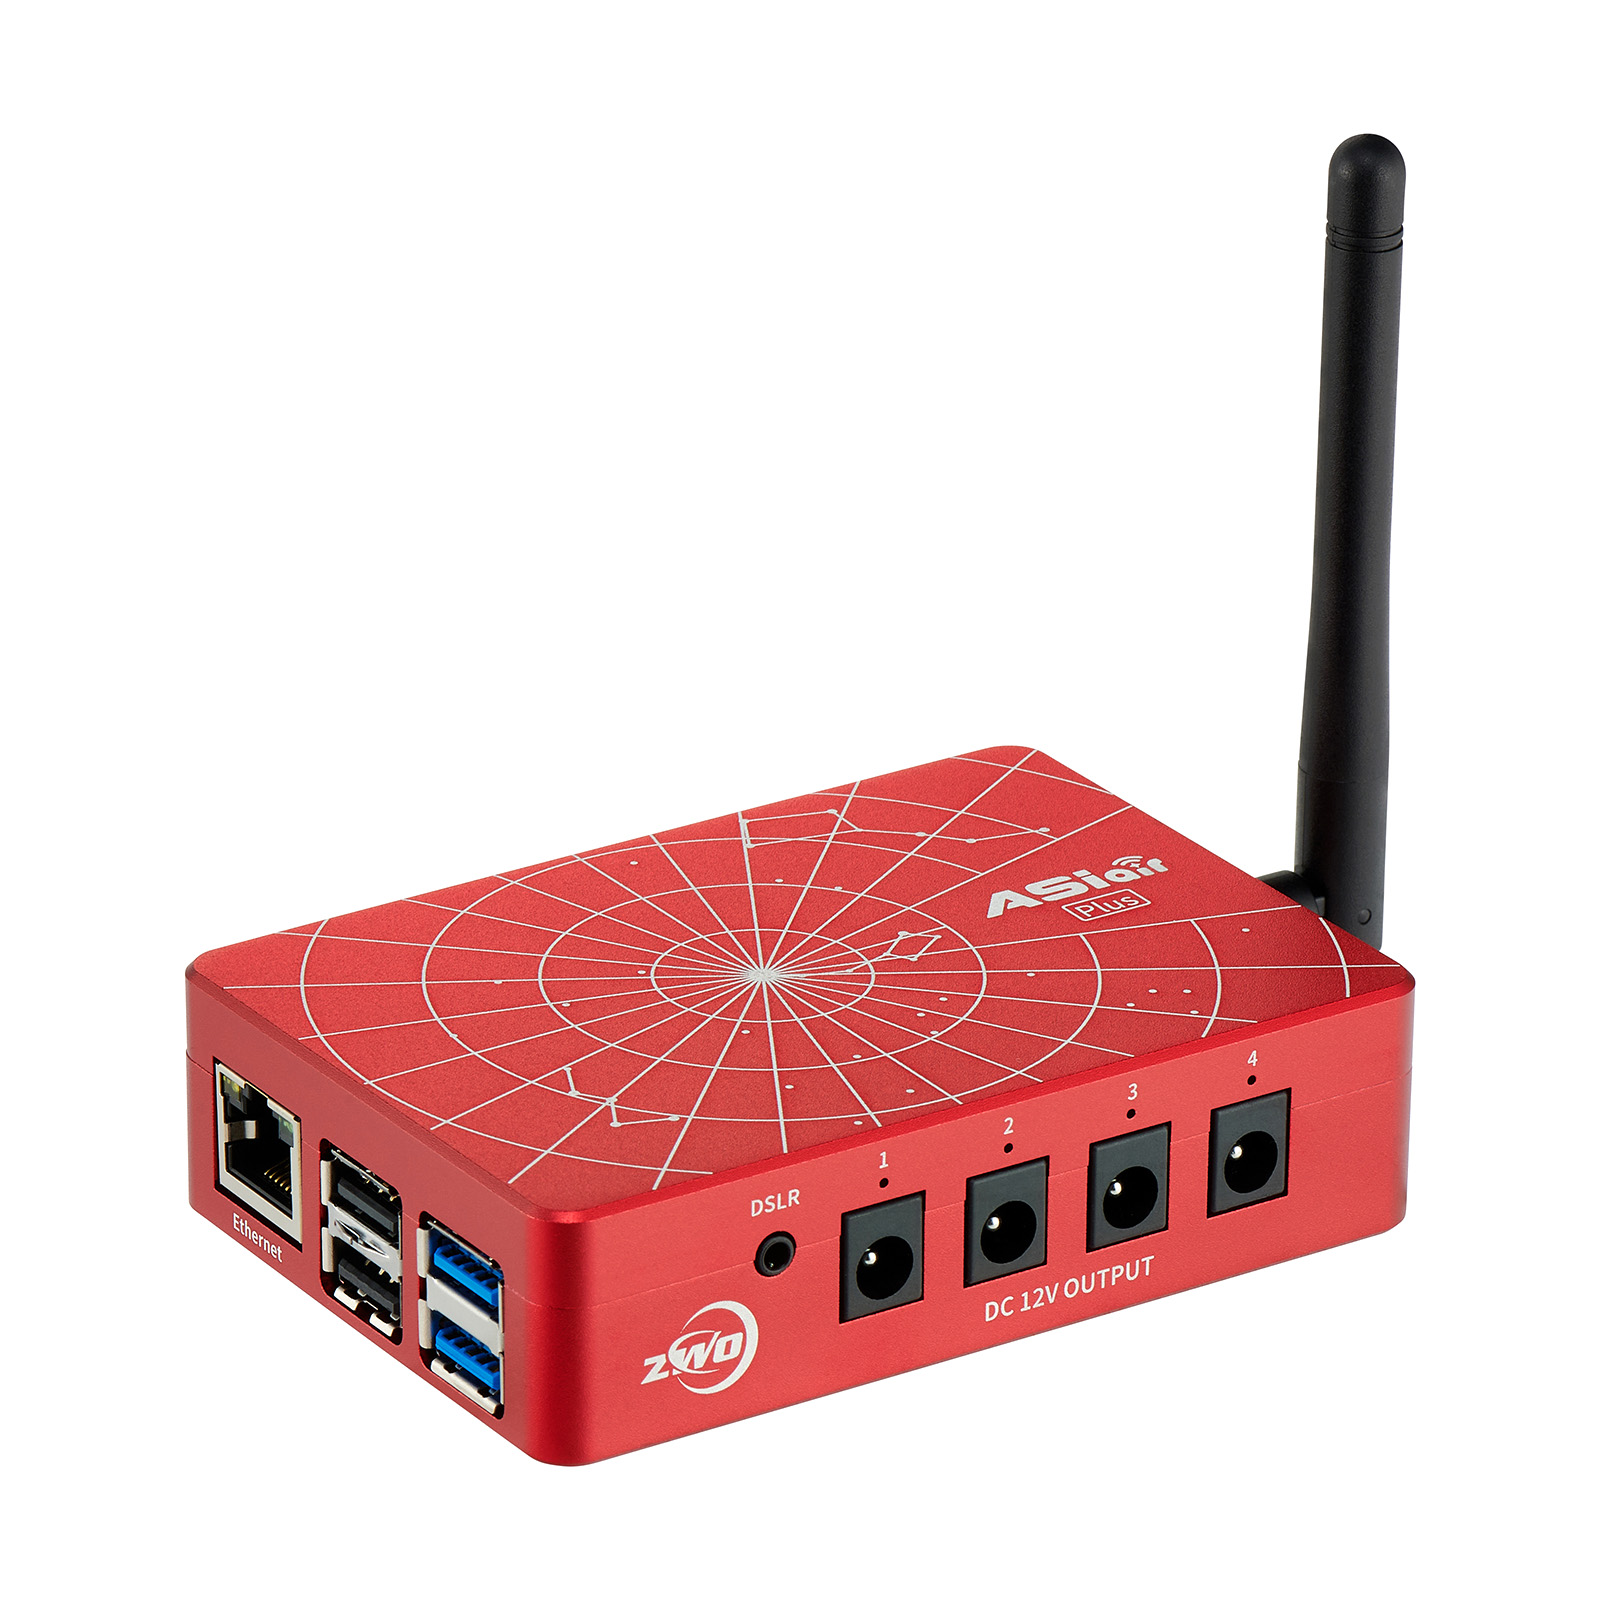
\includegraphics[height=0.50\textheight,width=\linewidth,keepaspectratio]{hw_art_state/zwo_asiair.jpg}\par
%         \vspace{0.03cm}
%         {\scriptsize ZWO ASIAIR [8].}
%         \column{0.32\textwidth}
%         \centering
%         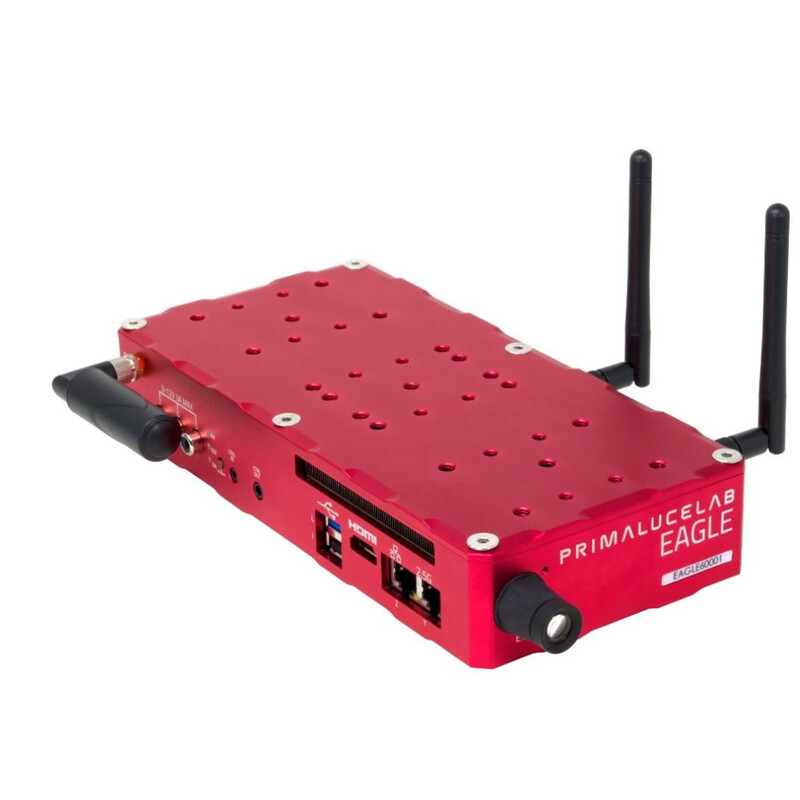
\includegraphics[height=0.50\textheight,width=\linewidth,keepaspectratio]{hw_art_state/primaLuceLab-Eagle6.jpg}\par
%         \vspace{0.03cm}
%         {\scriptsize PrimaLuceLab EAGLE6 [8].}
%         \column{0.32\textwidth}
%         \centering
%         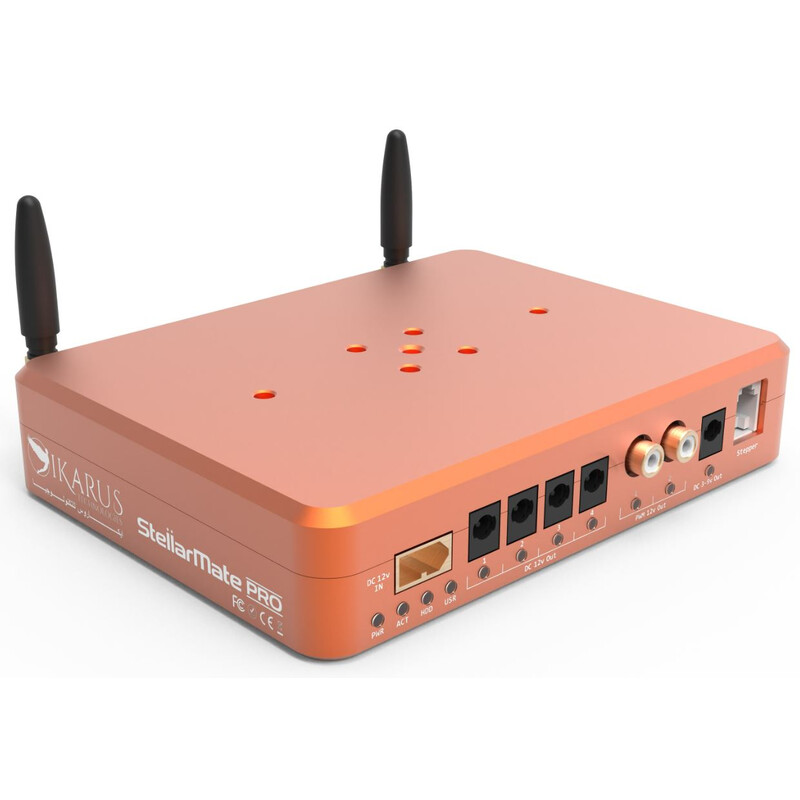
\includegraphics[height=0.50\textheight,width=\linewidth,keepaspectratio]{hw_art_state/stellar_mate-pro-8GB-128GB.jpg}\par
%         \vspace{0.03cm}
%         {\scriptsize StellarMate Pro [8].}
%     \end{columns}
    
%     \vfill
%     {\tiny\color{gray} [8] ZWO Optical Inc., “ASI Cameras Product Manual and Technical Integration Specifications,” v4.2, 2025.}
% \end{frame}

% \begin{frame}{Comparación de hardware comercial}
%     \centering
%     \circle
%     \small
%     \begin{table}
%         \centering
%         \setlength{\tabcolsep}{4pt}
%         \begin{tabular}{ll}
%             \toprule
%             \textbf{Sistema} & \textbf{Síntesis} \\
%             \midrule
%             ASIAIR & captura asistida, ecosistema cerrado, costo bajo--medio \\
%             EAGLE6 & PC astronómico robusto, múltiples puertos, costo alto \\
%             StellarMate & plataforma Linux abierta, automatización, costo medio \\
%             Prototipo & captura, registro, IA y predicción en flujo académico \\
%             \bottomrule
%         \end{tabular}
%     \end{table}
% \end{frame}

% \begin{frame}{Referencias Modernas de Detección y Clasificación}
%     \centering
    
%     \begin{columns}
%         \column{0.49\textwidth}
%         \centering
%         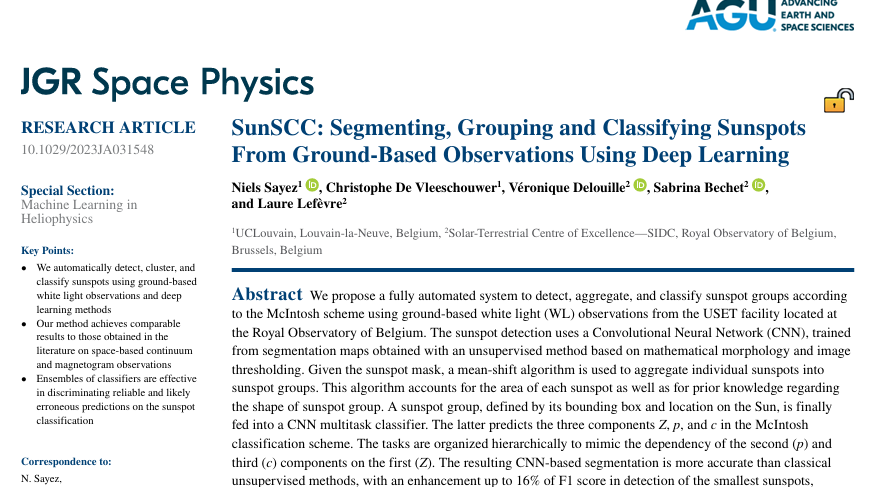
\includegraphics[height=0.62\textheight,width=\linewidth,keepaspectratio]{ref/etSayez.png}\par
%         \vspace{0.03cm}
%         {\scriptsize Article SunSCC--Automated solar classification dataset [4].}
%         \column{0.49\textwidth}
%         \centering
%         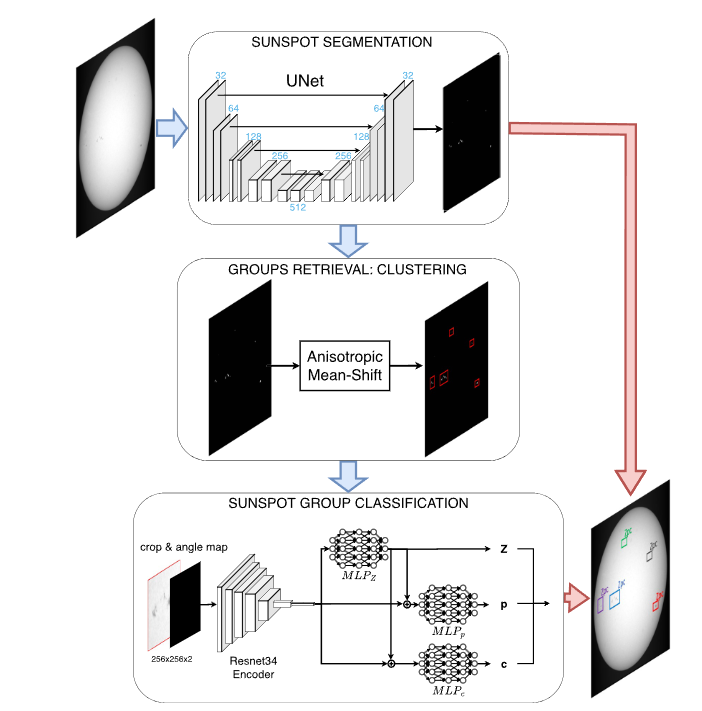
\includegraphics[height=0.6\textheight,width=\linewidth,keepaspectratio]{ml/yolo_train.png}\par
%         \vspace{0.03cm}
%         {\scriptsize Arquitectura modular de segmentacion, deteccion y clasificacion [4].}
%     \end{columns}
    
%     \vfill
%     {\tiny\color{gray} [4] M. Sayez et al., “SunSCC: Automated solar classification dataset,” Astronomy \& Astrophysics, 2023.}
% \end{frame}

% \begin{frame}{YOLO26--Etapa de Detección}
%     \centering
%     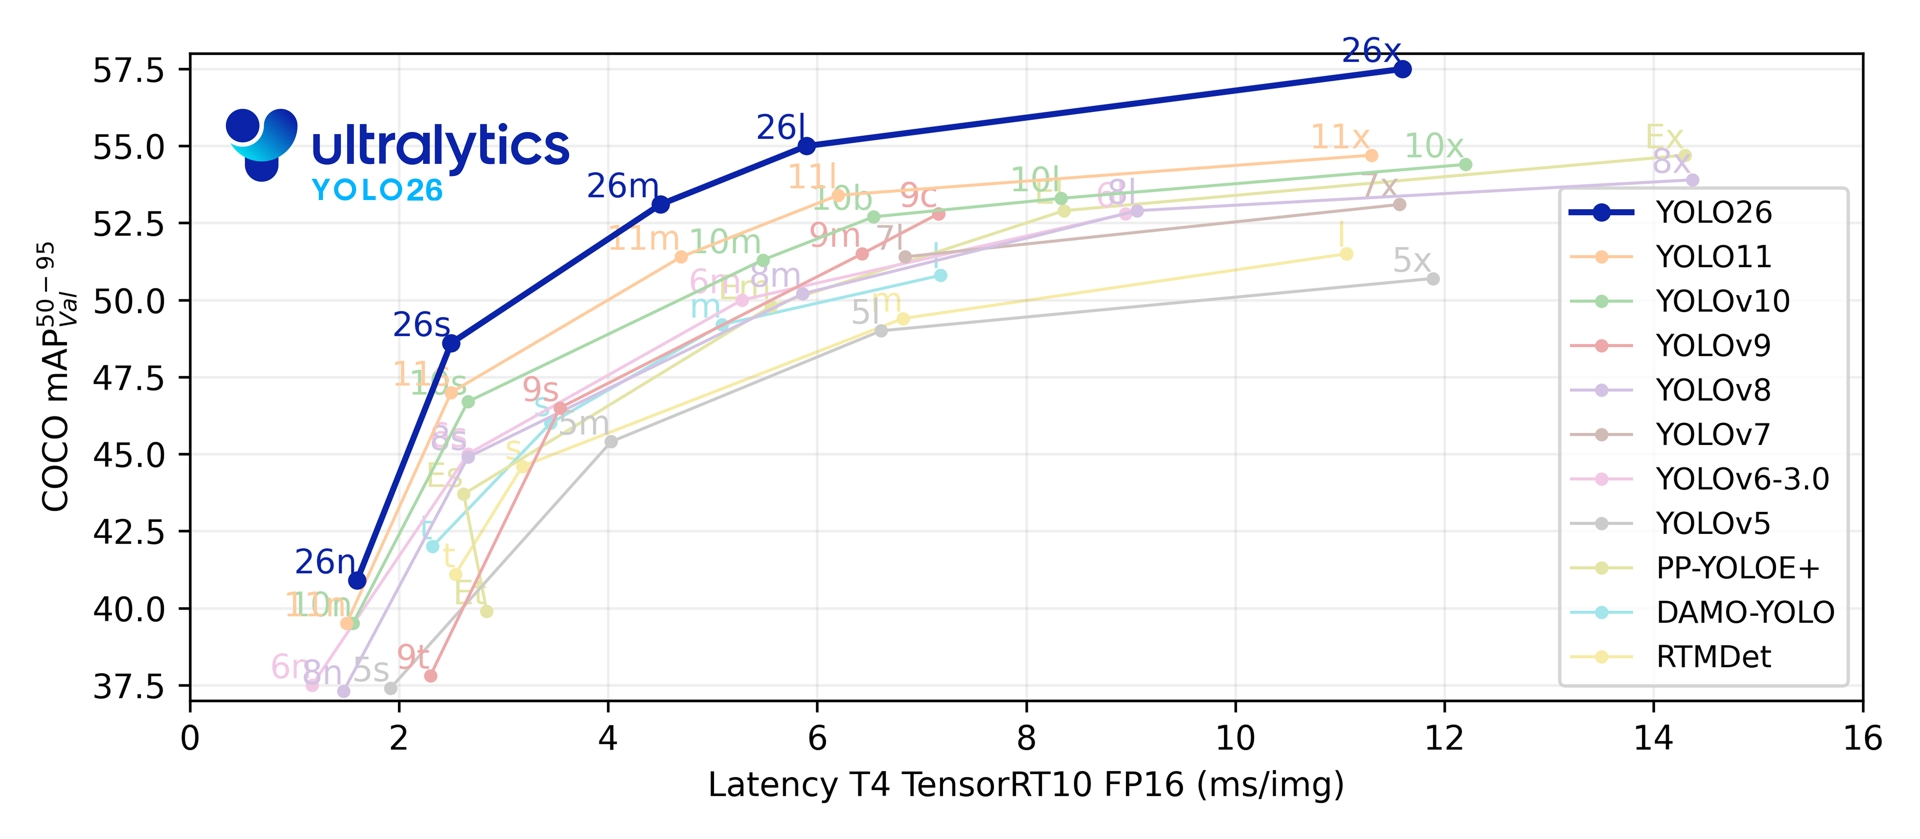
\includegraphics[height=0.62\textheight,width=0.96\linewidth,keepaspectratio]{ml/yolo_bench.jpg}\par
%     \vspace{0.05cm}
%     {\scriptsize Comparación de rendimiento de la familia YOLO [8].}
    
%     \vfill
%     {\tiny\color{gray} [8] Ultralytics LLC, “YOLO26 Real-Time Object Detection Engine and Benchmarks,” 2026.}
% \end{frame}

% \begin{frame}{ConvNeXtV2--Etapa de Clasificación}
%     \begin{columns}
%         \column{0.49\textwidth}
%         \centering
%         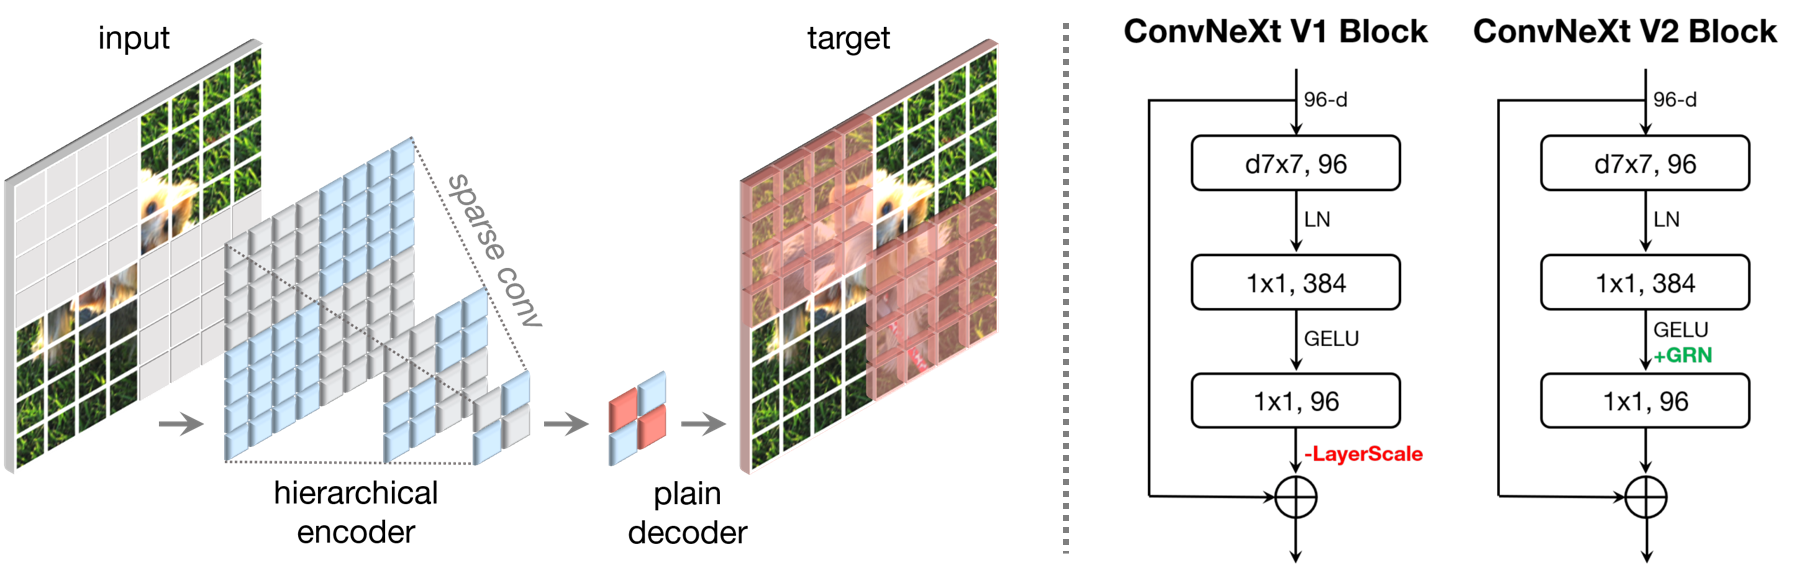
\includegraphics[height=0.54\textheight,width=\linewidth,keepaspectratio]{ml/fcmae.png}\par
%         \vspace{0.03cm}
%         {\scriptsize Preentrenamiento FCMAE [10].}
%         \column{0.49\textwidth}
%         \centering
%         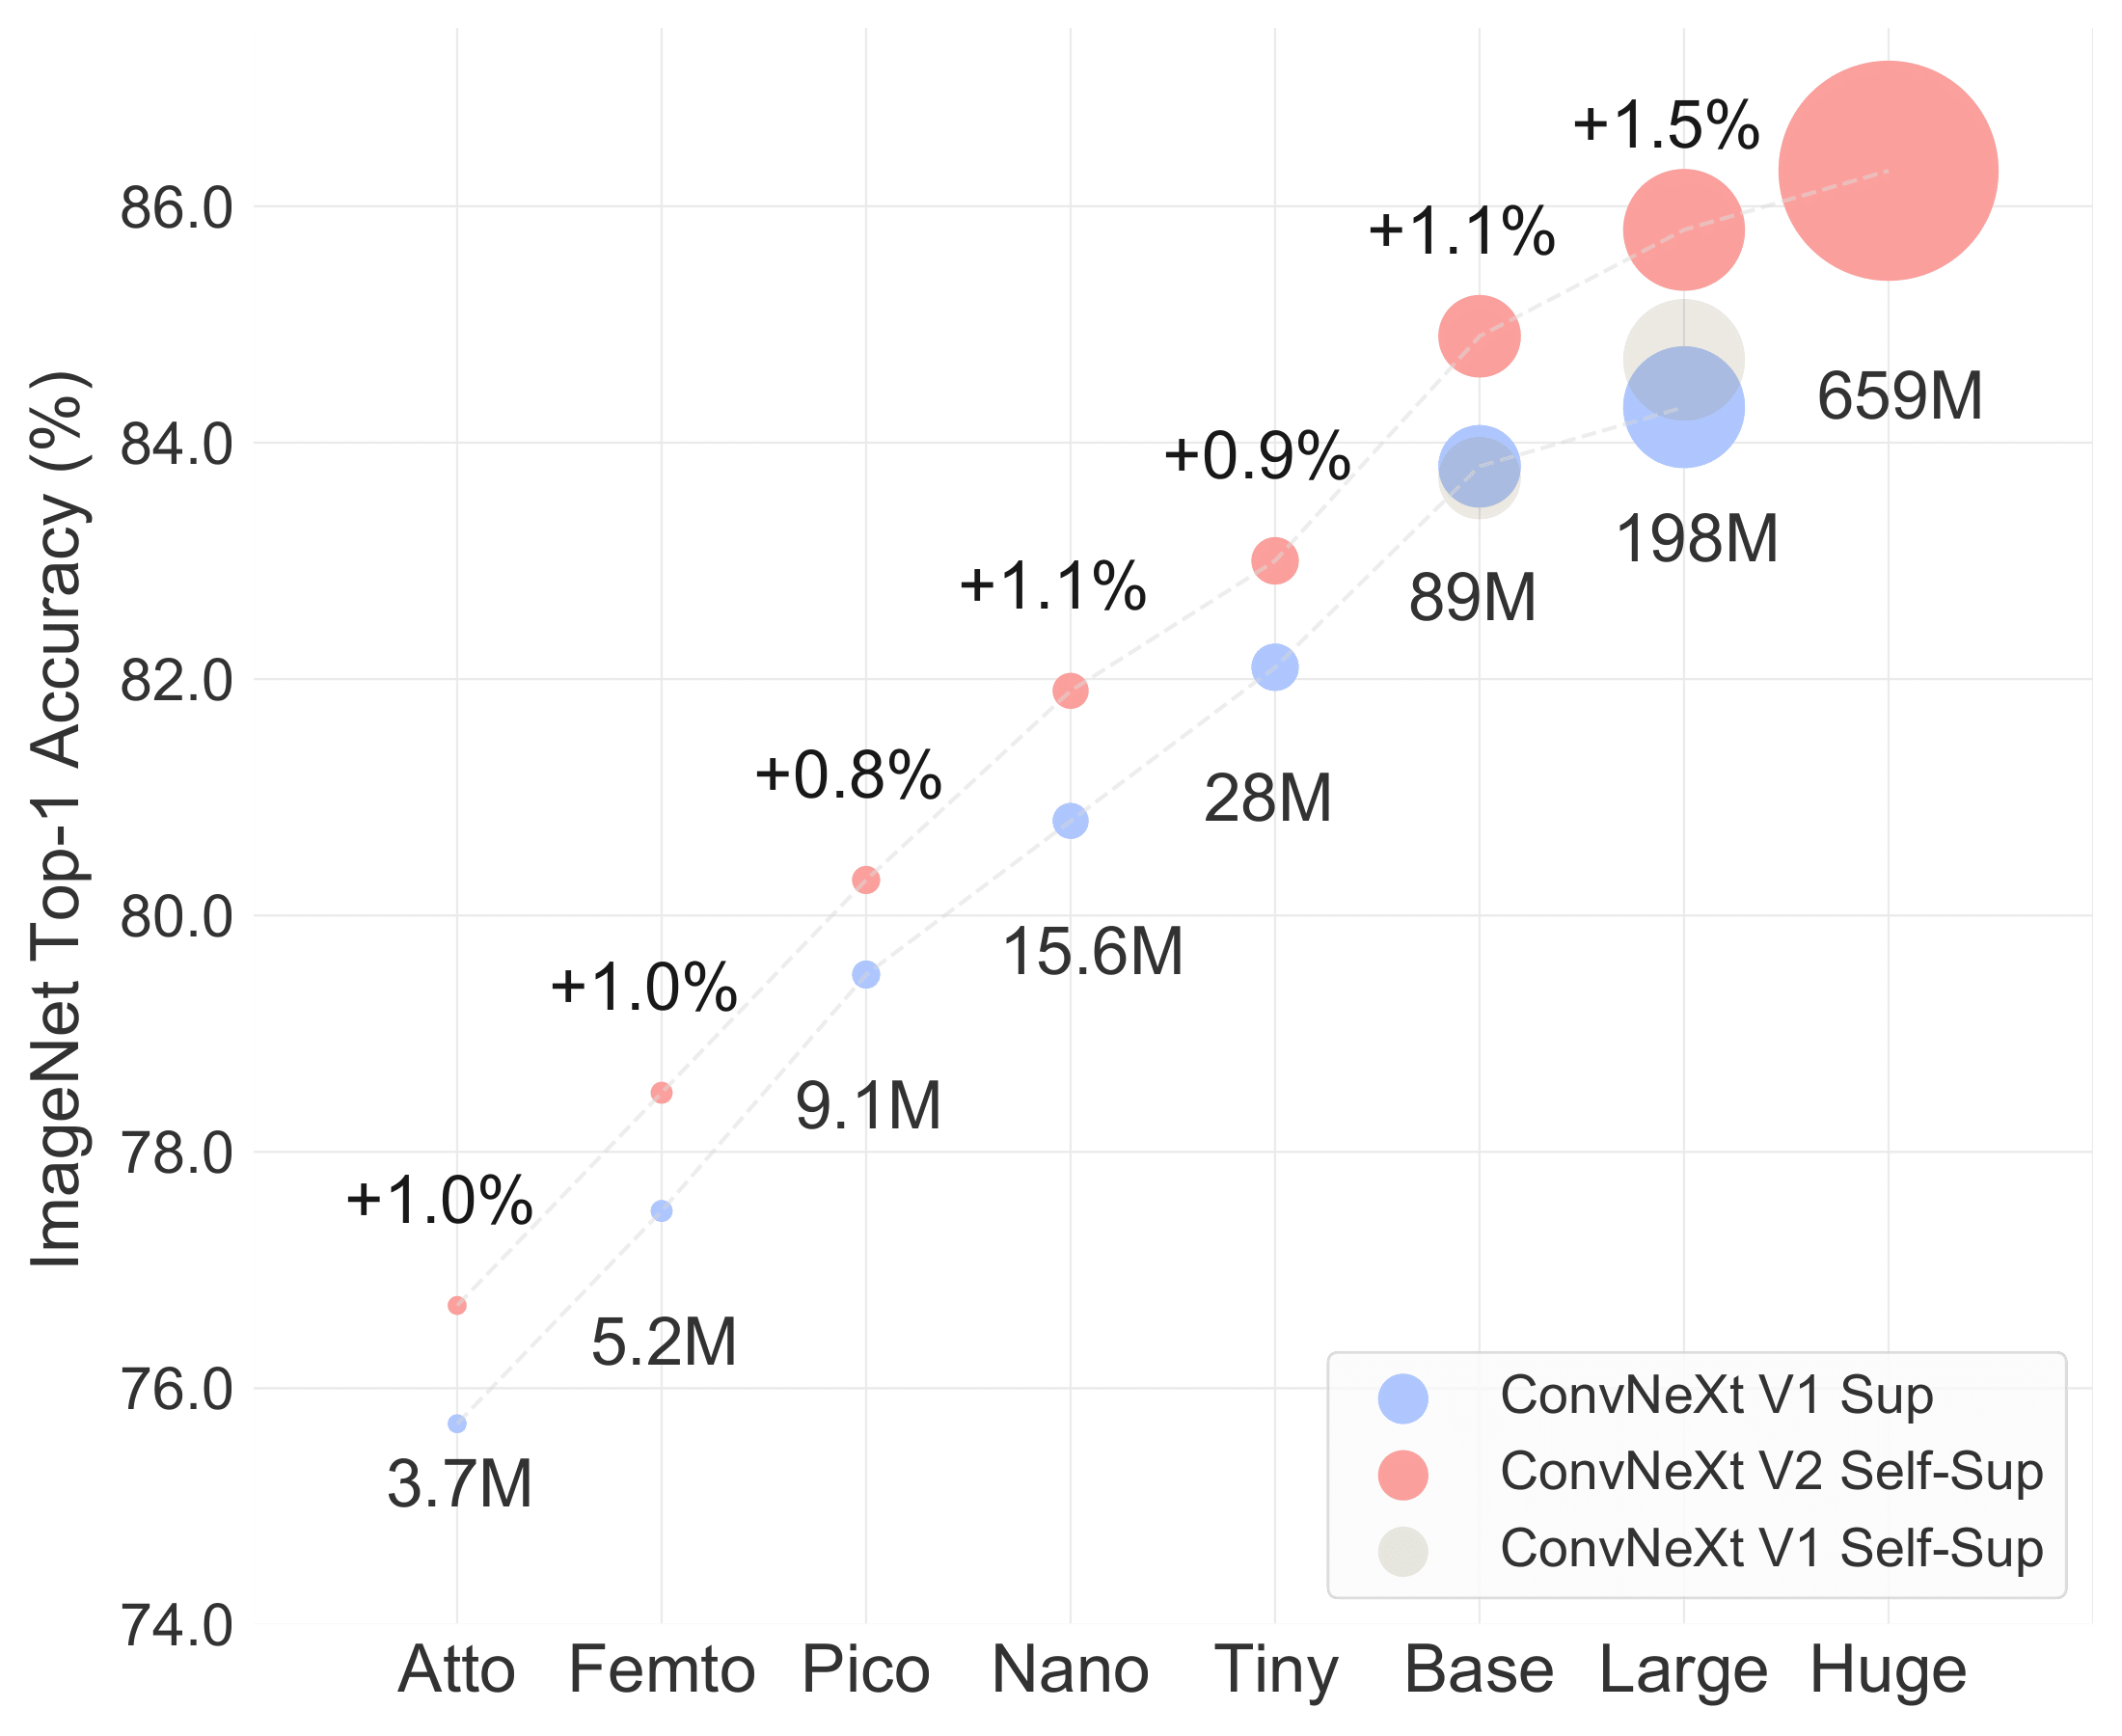
\includegraphics[height=0.54\textheight,width=\linewidth,keepaspectratio]{ml/scaling.png}\par
%         \vspace{0.03cm}
%         {\scriptsize Escalamiento ConvNeXtV2 [10].}
%     \end{columns}
    
%     \vfill
%     {\tiny\color{gray} [10] S. Woo et al., “ConvNeXt V2: Co-designing and scaling convnets with masked autoencoders,” in Proc. IEEE/CVF CVPR, 2023, pp. 16133--16142.}
% \end{frame}

% \begin{frame}{Modelos Predictivos}
%     \vspace{0.1cm}

%     \begin{columns}[c, onlytextwidth]
%         \begin{column}{0.48\textwidth}
%             \centering
%             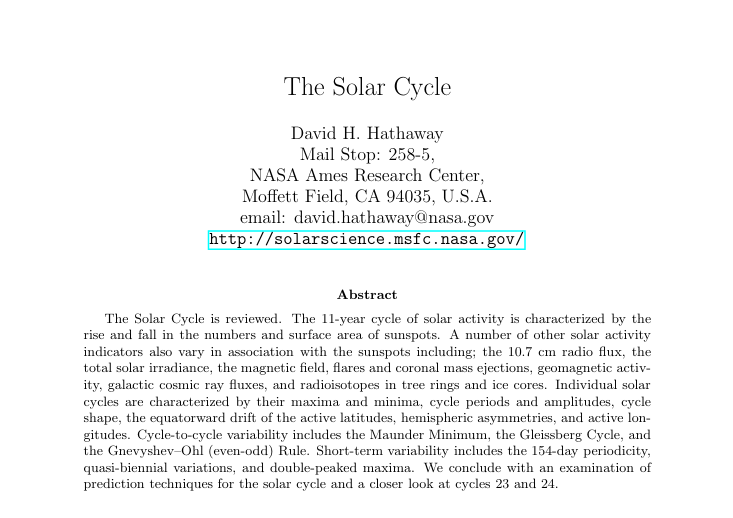
\includegraphics[height=0.55\textheight,width=\linewidth,keepaspectratio]{ref/etHathaway.png}\par
%             \vspace{0.05cm}
%             {\scriptsize Article The Solar Cycle [7].}
%         \end{column}
        
%         \hfill
        
%         \begin{column}{0.48\textwidth}
%             \centering
%             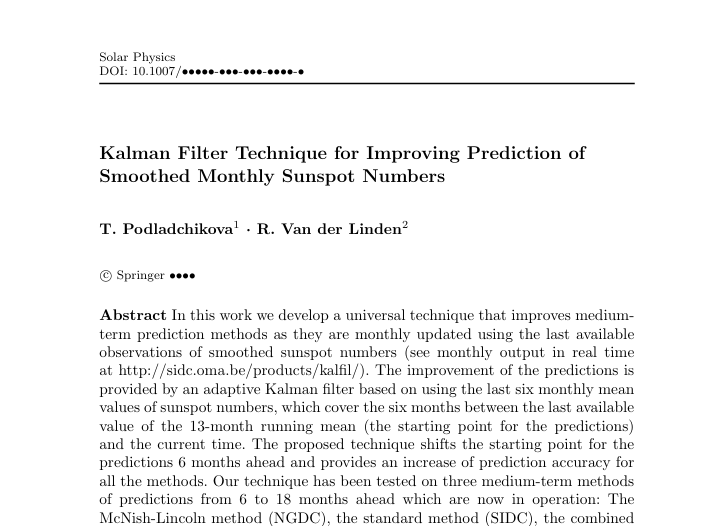
\includegraphics[height=0.55\textheight,width=\linewidth,keepaspectratio]{ref/etPLV.png}\par
%             \vspace{0.05cm}
%             {\scriptsize Article Kalman Filter Technique for SSN Improving Prediction [11].}
%         \end{column}
%     \end{columns}

%     \vfill

%     % Al agrupar todo dentro de un mismo bloque { }, el interlineado de tiny se aplica a todo el conjunto
%     {\tiny\color{gray} 
%     [7] D. H. Hathaway, “The solar cycle,” Living Reviews in Solar Physics, vol. 12, no. 1, pp. 1--70, 2015. \par\vspace{0.05cm}
%     [11] Podladchikova, T. y Van der Linden, R. (2011). Kalman Filter Technique for Improving Prediction of Smoothed Monthly Sunspot Numbers. Solar Physics, 271(2), 469–485.\par}
% \end{frame}

\section{Projeto de Hardware}

\begin{frame}{Módulo de Observação \quad \setlength{\fboxrule}{1.2pt}\setlength{\fboxsep}{3pt}\raisebox{0.1ex}{\fcolorbox{llamativoMagenta}{white}{\scriptsize\textcolor{llamativoMagenta}{\textbf{Contribuição 1}}}}}
    
    % --- CONTENIDO PRINCIPAL ---
    \centering
    \vfill
    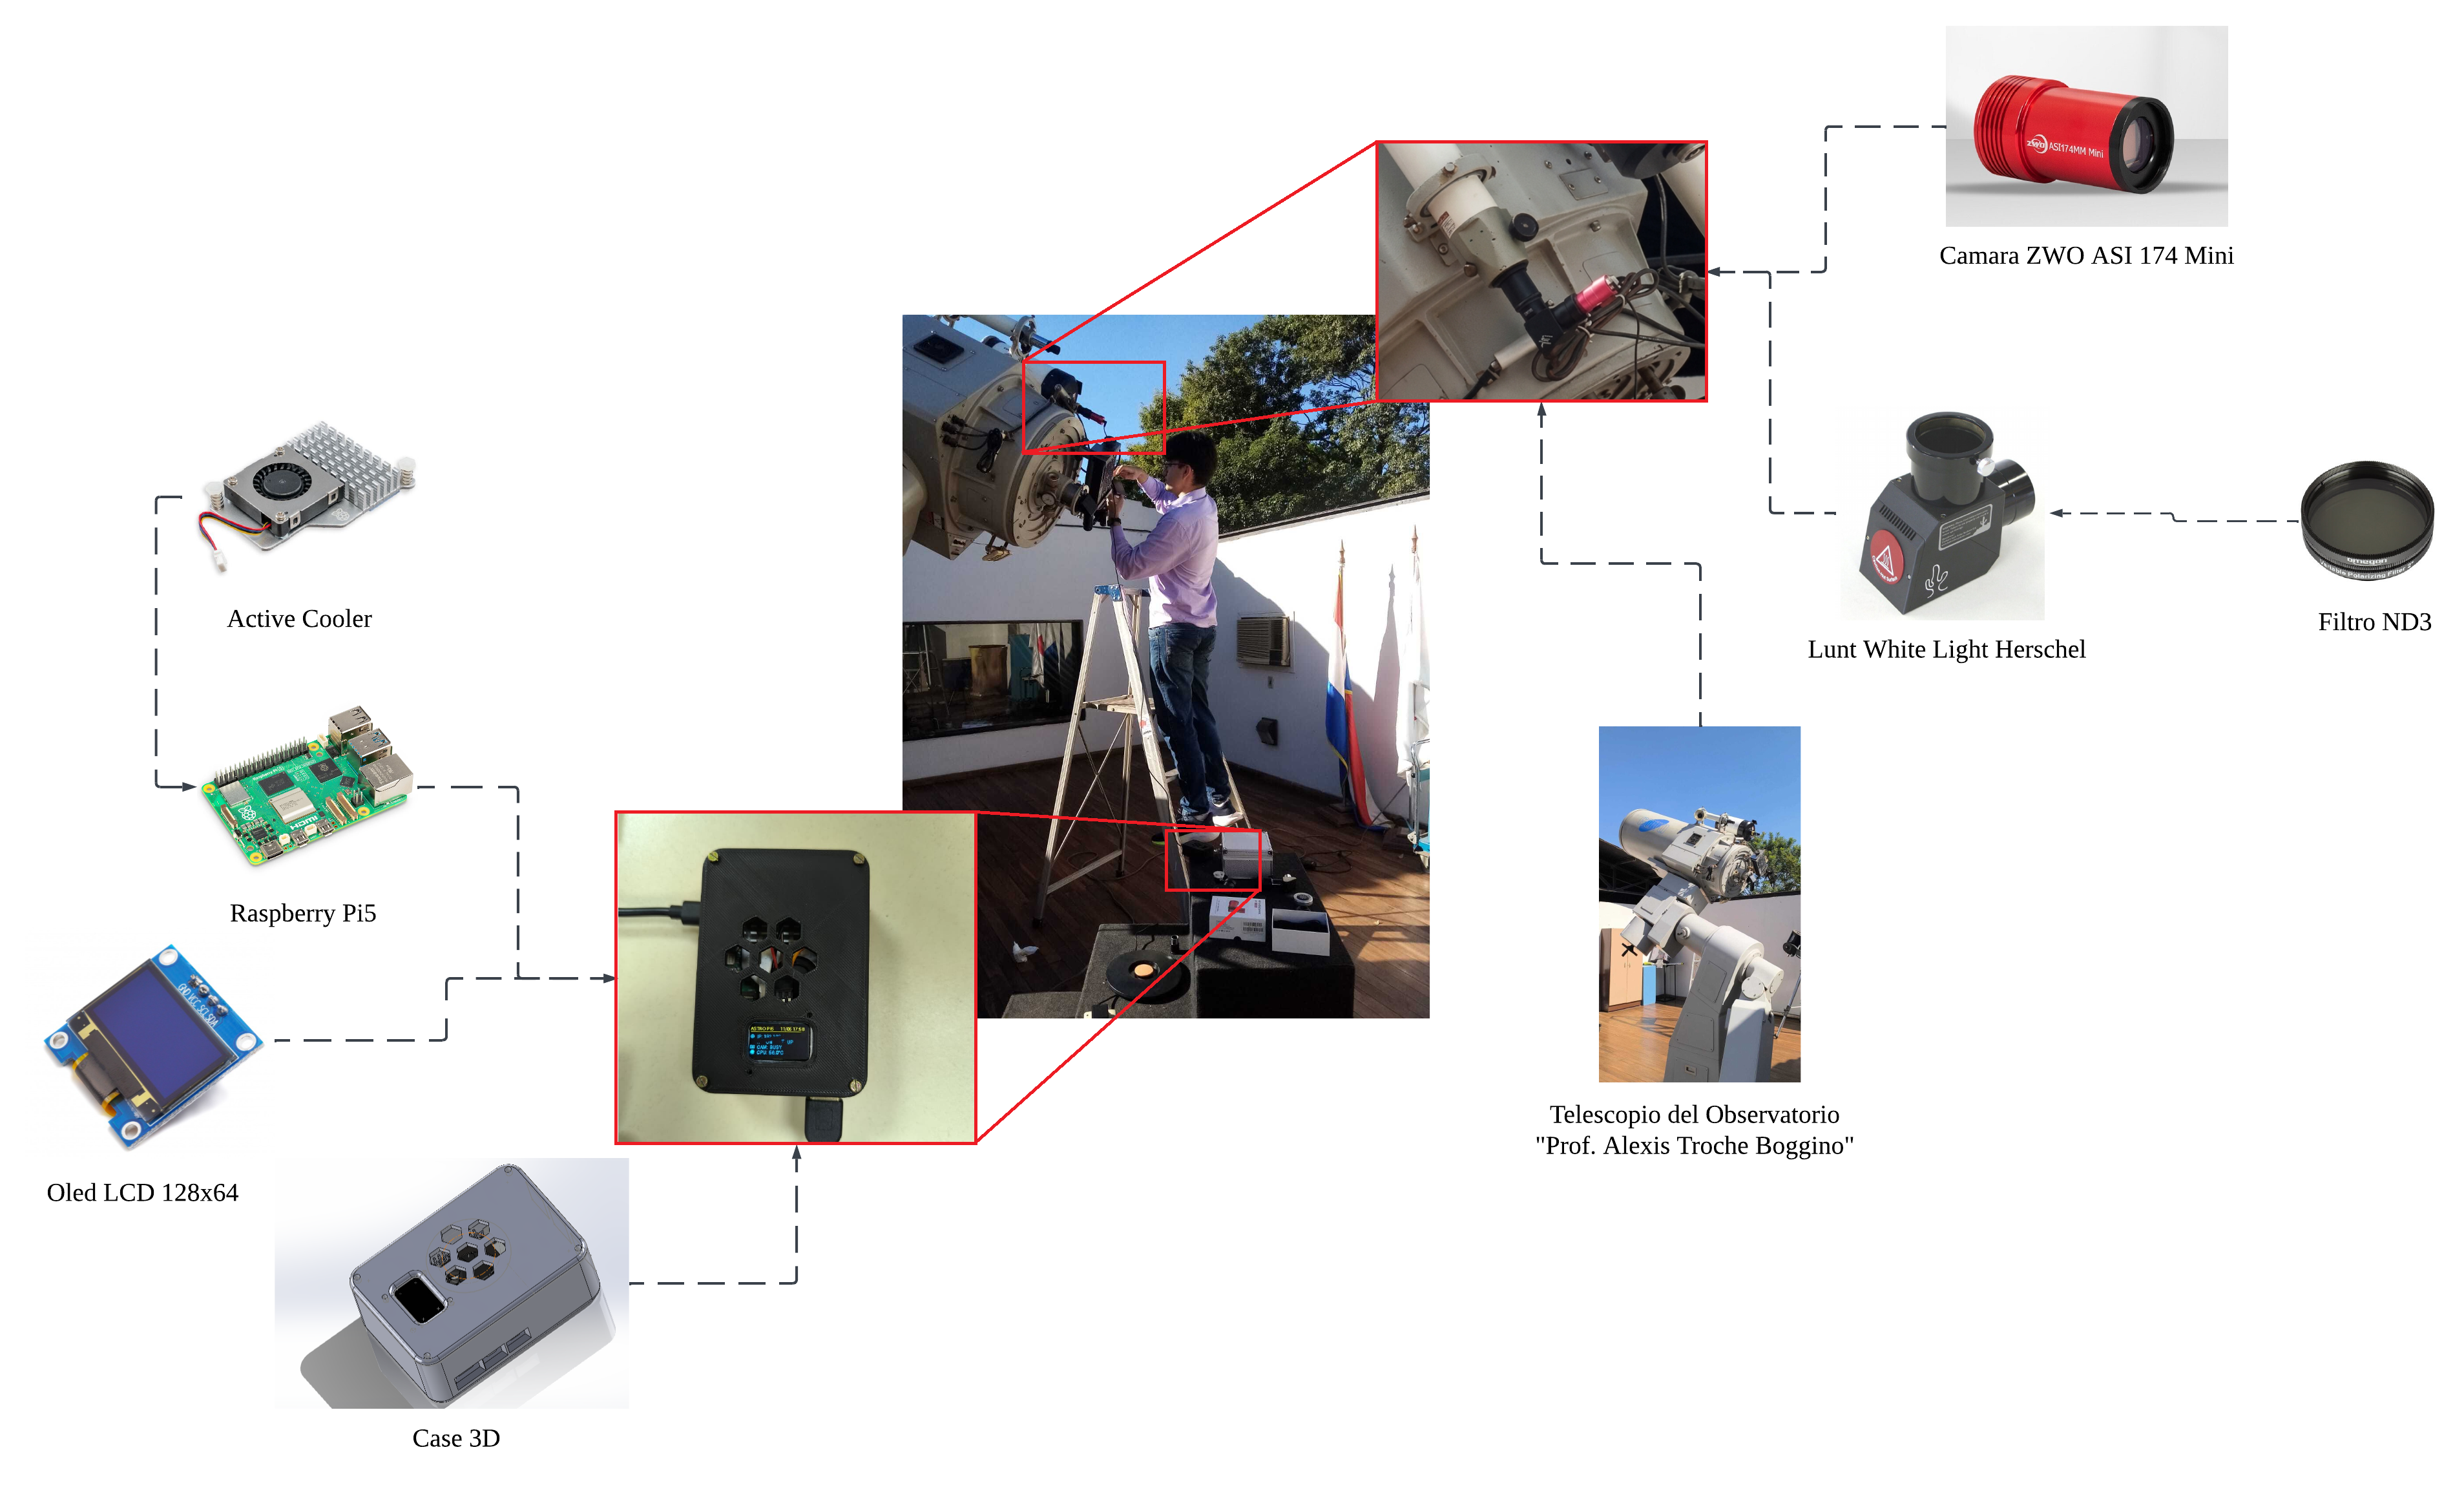
\includegraphics[height=0.82\textheight, width=0.98\linewidth, keepaspectratio]{hw/hw_diagram.png}
    \vfill
    
\end{frame}

\begin{frame}{Projeto CAD e Integração de Hardware}
    \centering
    \begin{columns}[c]
        \begin{column}{0.32\linewidth}
            \centering
            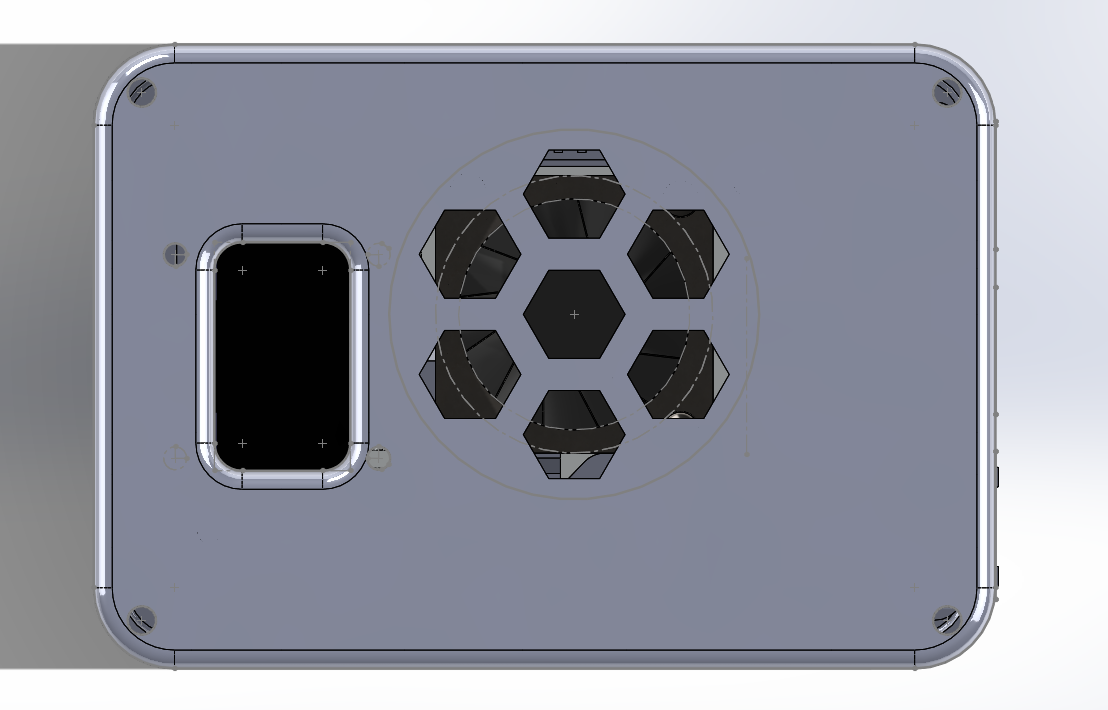
\includegraphics[width=\linewidth,height=0.55\textheight,keepaspectratio]{cad/case_lid.png}\par
            \vspace{0.05cm}
            {\scriptsize Gabinete externo fechado}
        \end{column}
        \begin{column}{0.32\linewidth}
            \centering
            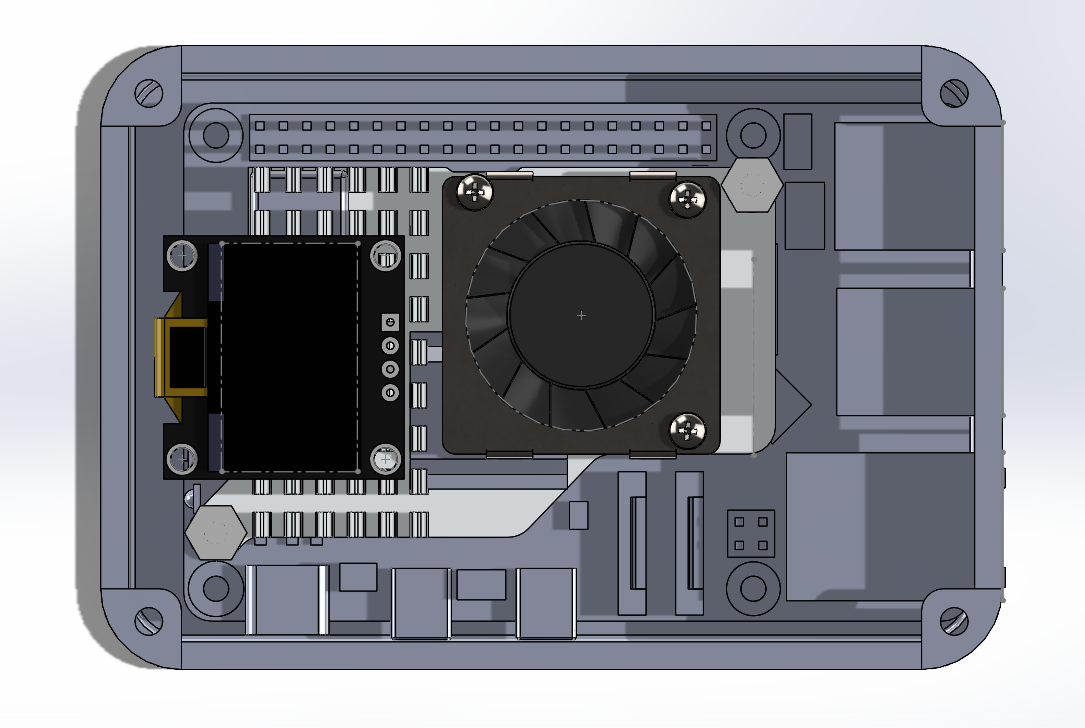
\includegraphics[width=\linewidth,height=0.55\textheight,keepaspectratio]{cad/case_open.png}\par
            \vspace{0.05cm}
            {\scriptsize Disposição interna CAD}
        \end{column}
        \begin{column}{0.32\linewidth}
            \centering
            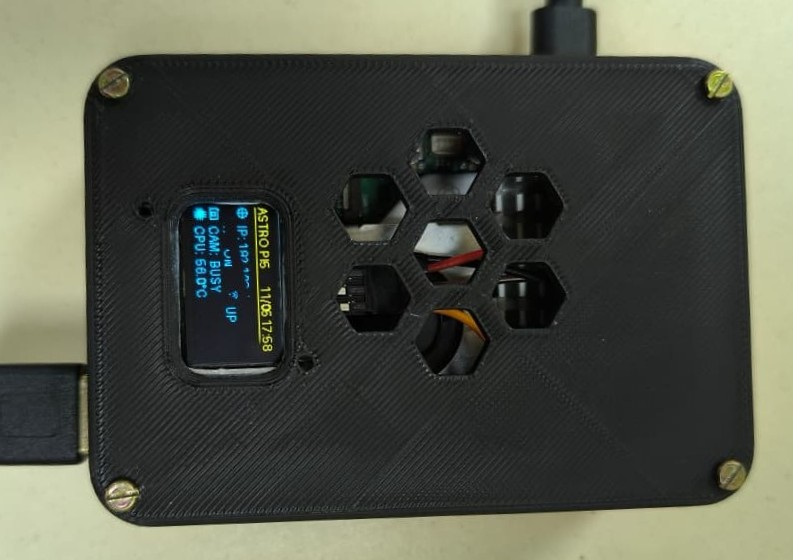
\includegraphics[width=\linewidth,height=0.55\textheight,keepaspectratio]{hw/obs_module.jpeg}\par
            \vspace{0.05cm}
            {\scriptsize Protótipo físico fabricado}
        \end{column}
    \end{columns}\par
    
    \vspace{0.25cm}
    {\footnotesize\color{black!85} Modelagem no SolidWorks e manufatura aditiva (impressão 3D PETG) do módulo de aquisição local e processamento embarcado.}
\end{frame}

\section{Projeto de Software}

\begin{frame}{Dados de Treinamento: HMI/SDO + SRS/NOAA}
    \centering
    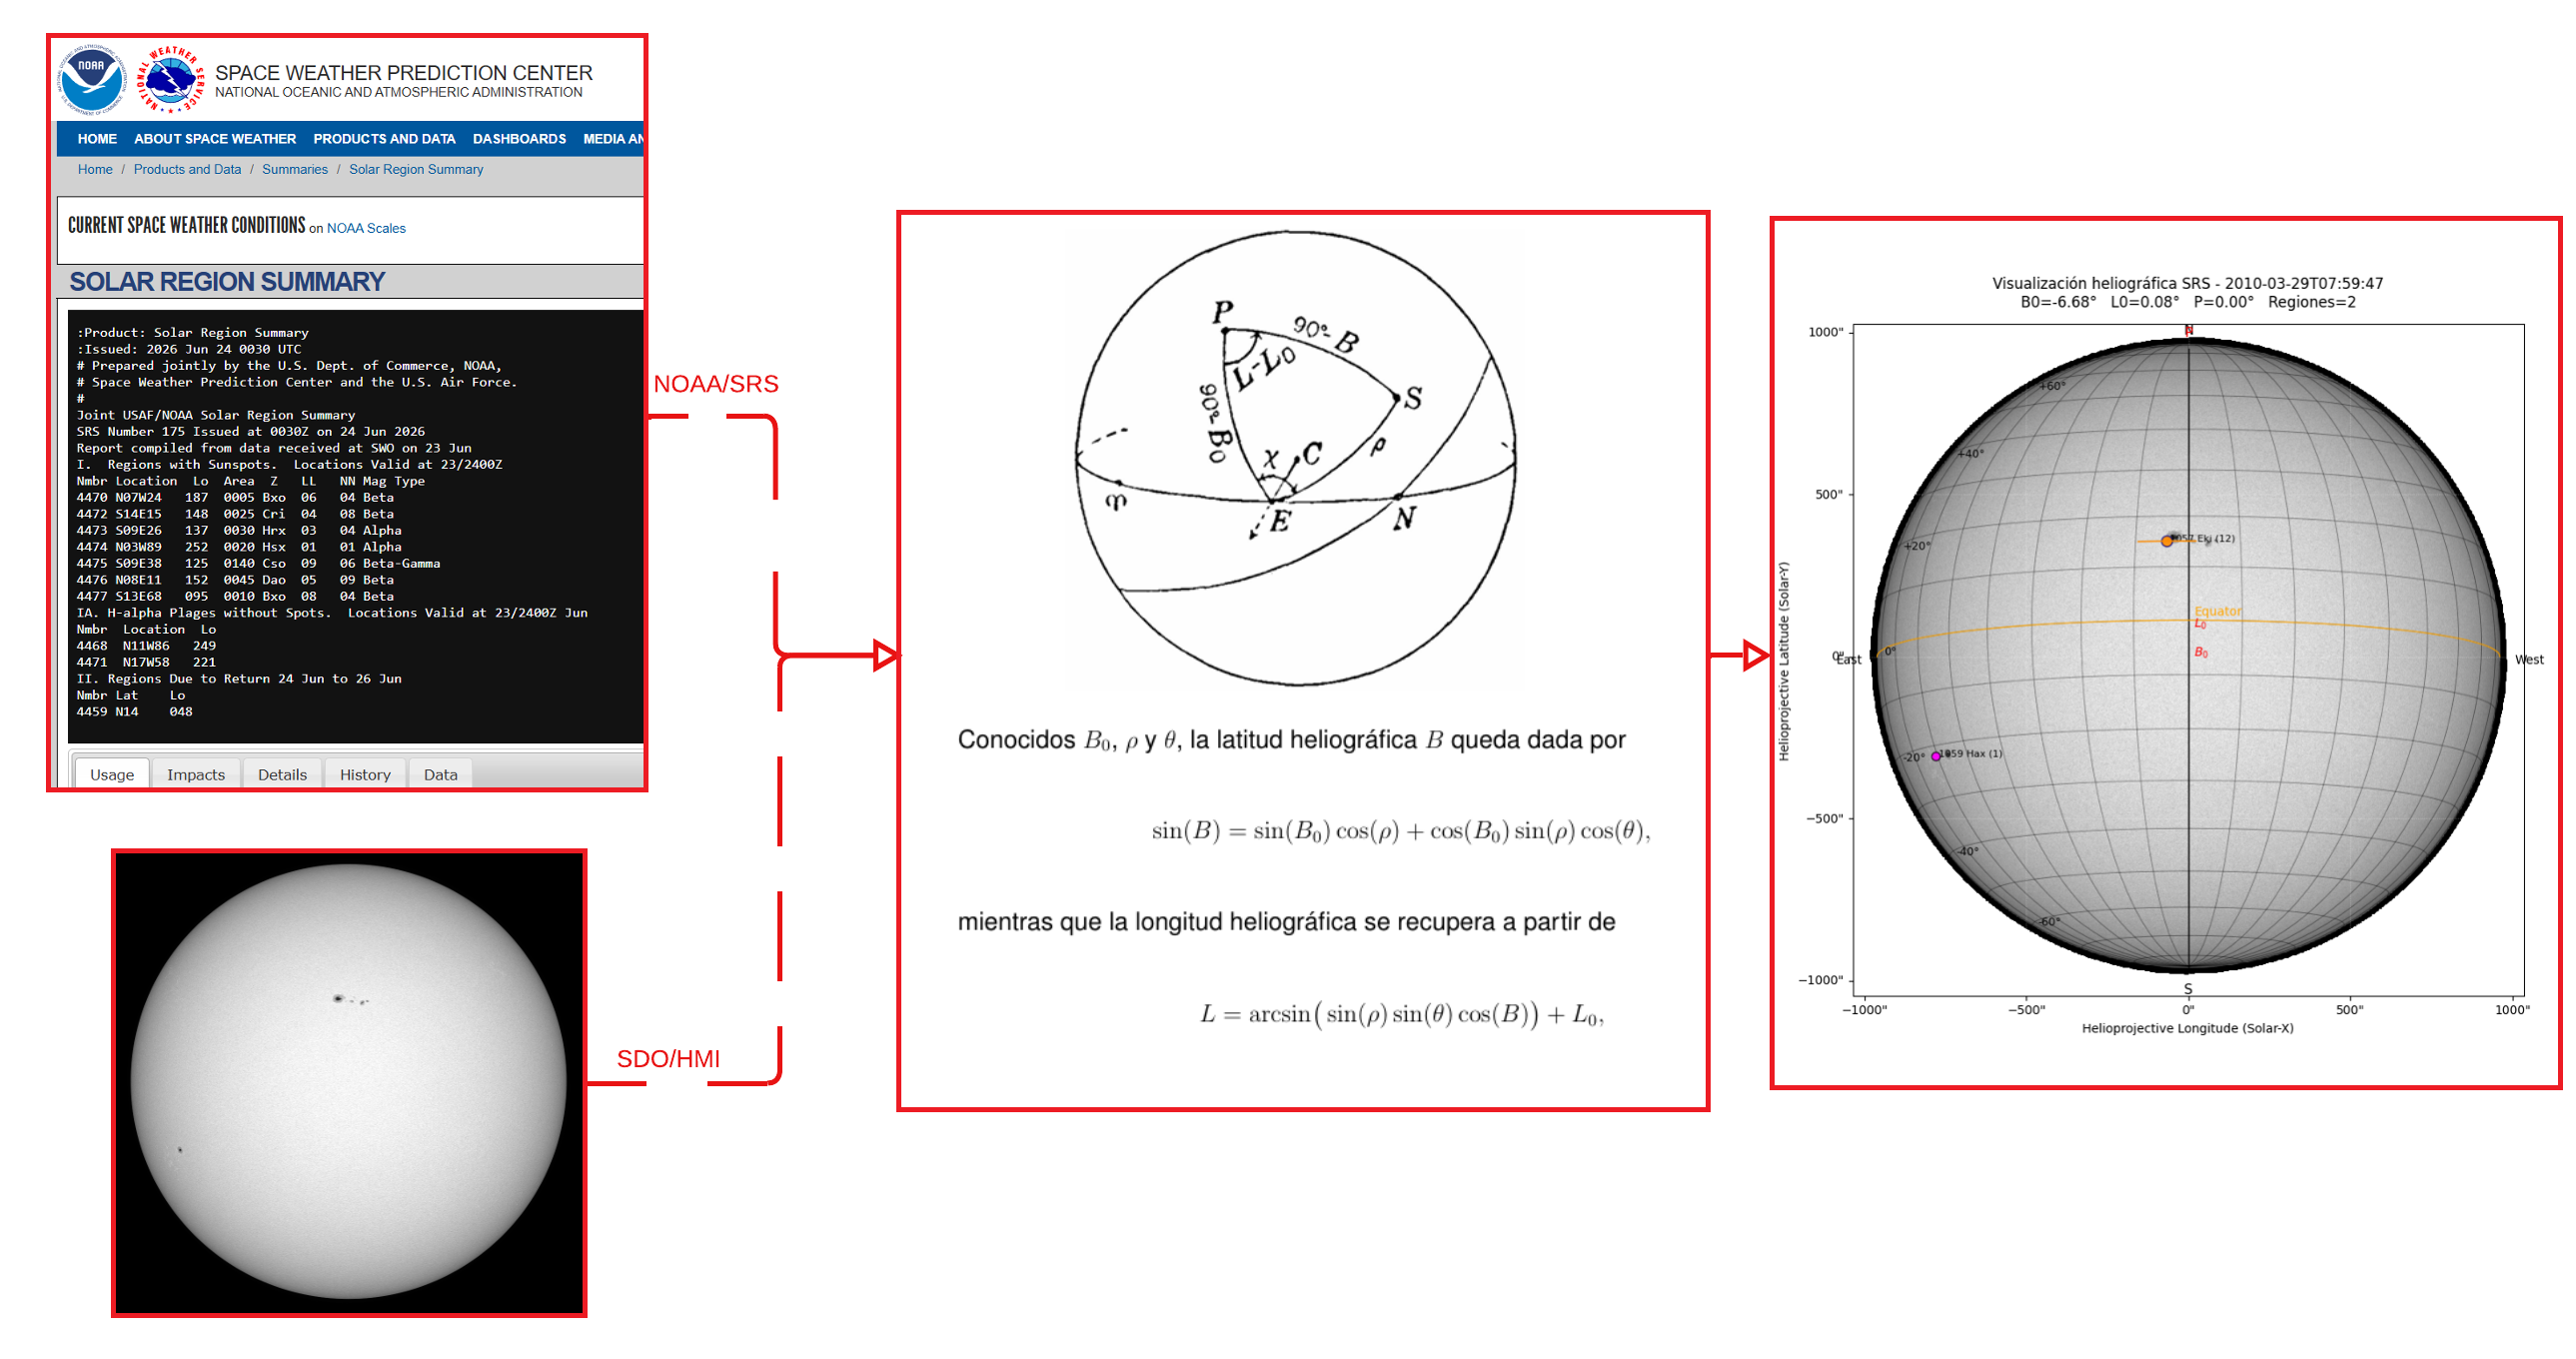
\includegraphics[height=0.86\textheight,width=\linewidth,keepaspectratio]{data/blockDiagram_DB.png}
    \vspace{0.08cm}
\end{frame}

\begin{frame}{Dados de Treinamento: Discretização da Base de Dados}
    \centering
    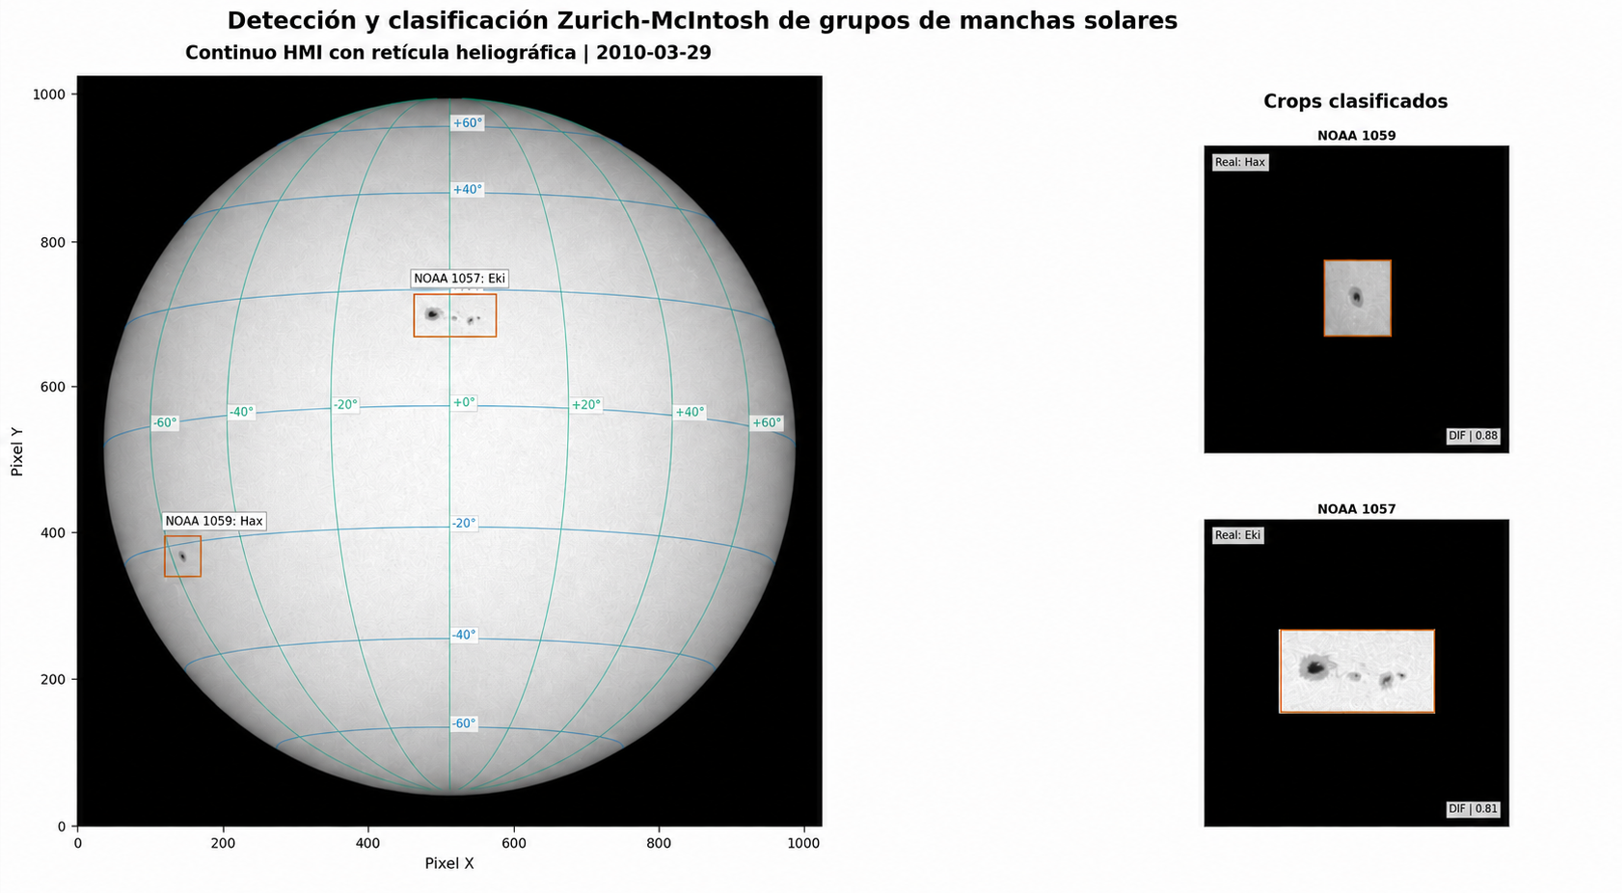
\includegraphics[height=0.9\textheight,width=0.92\linewidth,keepaspectratio]{data/db2_build.png}
    \vspace{0.08cm}
\end{frame}

\begin{frame}{Dados de Treinamento: Datasets gerados (2010--2025) \quad \setlength{\fboxrule}{1.2pt}\setlength{\fboxsep}{3pt}\raisebox{0.1ex}{\fcolorbox{llamativoMagenta}{white}{\scriptsize\textcolor{llamativoMagenta}{\textbf{Contribuição 2}}}}}
    \footnotesize
    \begin{block}{DB1 -- detecção de grupos solares (Para YOLO26n)}
      \begin{itemize}
            \item \textbf{4700 imagens} de disco solar completo em \textbf{1024\,$\times$\,1024 px}.
            \item Inclui \textit{bounding boxes} de agrupamento solar para treinamento tipo YOLO.
      \end{itemize}
    \end{block}

    \begin{block}{DB2 -- classificação morfológica (Etapa preliminar)}
        \begin{itemize}
            \item \textbf{15000 recortes} derivados dos \textit{bounding boxes} de DB1 em \textbf{224\,$\times$\,224 px}.
            \item Inclui rótulos $ZPC$ de SRS/NOAA [5].
        \end{itemize}
    \end{block}

    \begin{block}{DB2.1 -- classificação morfológica refinada (Para ConvNeXtV2a)}
        \begin{itemize}
            \item \textbf{14700 recortes} derivados de DB2 em \textbf{224\,$\times$\,224 px} refinados com \textbf{PCA} de 60 componentes principais e Isolation Forest.
            \item Inclui rótulos $ZPC$ de SRS/NOAA [5].
        \end{itemize}
    \end{block}
    
    \vfill
    {\raggedright\tiny\color{gray} [5] NOAA Space Weather Prediction Center, “Solar Region Summary (SRS) Data Logs,” 2025.\par}
\end{frame}


% \begin{frame}{Modelos predictivos: Modelo escalar de Podladchikova con filtro Kalman (PVLK)}
%     \centering
%     \small
    
%     \vspace{0.1cm}
%     \begin{columns}[T]
%         % Columna Izquierda: Ecuaciones y flujo del filtro
%         \begin{column}{0.65\textwidth}
%             \footnotesize
%             \textbf{1. Modelo Paramétrico PVL (Forma del ciclo):}
%             \begin{equation*}
%                 f(v; a, b) = \frac{a \cdot v^3}{\exp(v^2/b^2) - 0.71} \quad \text{con } b=27.12 + 25.15(1000a)^{-1/4}
%             \end{equation*}

%             \textbf{2. Ruido Adaptativo e Inyección de $Q_k$:}
%             \begin{equation*}
%                 Q_k = 0.2 \Phi_k \hat{s}_{k-1}, \quad R_k = 2.5 \Phi_k \hat{s}_{k-1} \quad \rightarrow \quad P_k^- = \Phi_k^2 P_{k-1} + Q_k
%             \end{equation*}

%             \textbf{3. Ganancia de Kalman ($K_k$) y Actualización:}
%             \begin{equation*}
%                 K_k = \frac{P_k^-}{P_k^- + R_k} \quad \rightarrow \quad \hat{s}_k = \Phi_k \hat{s}_{k-1} + K_k (z_k - \Phi_k \hat{s}_{k-1})
%             \end{equation*}
%         \end{column}
        
%         % Columna Derecha: Tabla de variables optimizada
%         \begin{column}{0.32\textwidth}
%             \vspace{0.3cm}
%             \centering
%             \footnotesize
%             \renewcommand{\arraystretch}{1.2}
%             \begin{tabular}{c|l}
%                 \textbf{Var.} & \textbf{Descripción} \\ \hline
%                 $v$ & Tiempo (meses) \\
%                 $a, b$ & Parámetros PVL \\
%                 $\Phi_k$ & Transición: $\frac{f(v_k)}{f(v_{k-1})}$ \\
%                 $\hat{s}_k$ & Estado ($SSN_{\mathrm{PVLK}}$) \\
%                 $P_k$ & Varianza del error \\
%                 $z_k$ & Medición real (SSN) \\
%             \end{tabular}
%         \end{column}
%     \end{columns}

%     \vspace{0.3cm}
    
\begin{frame}{Modelos Preditivos: Vetorização e DMD \quad \setlength{\fboxrule}{1.2pt}\setlength{\fboxsep}{3pt}\raisebox{0.1ex}{\fcolorbox{llamativoMagenta}{white}{\scriptsize\textcolor{llamativoMagenta}{\textbf{Contribuição 3}}}}}
    \centering
    \vspace{-0.28cm}
    \makebox[\linewidth][c]{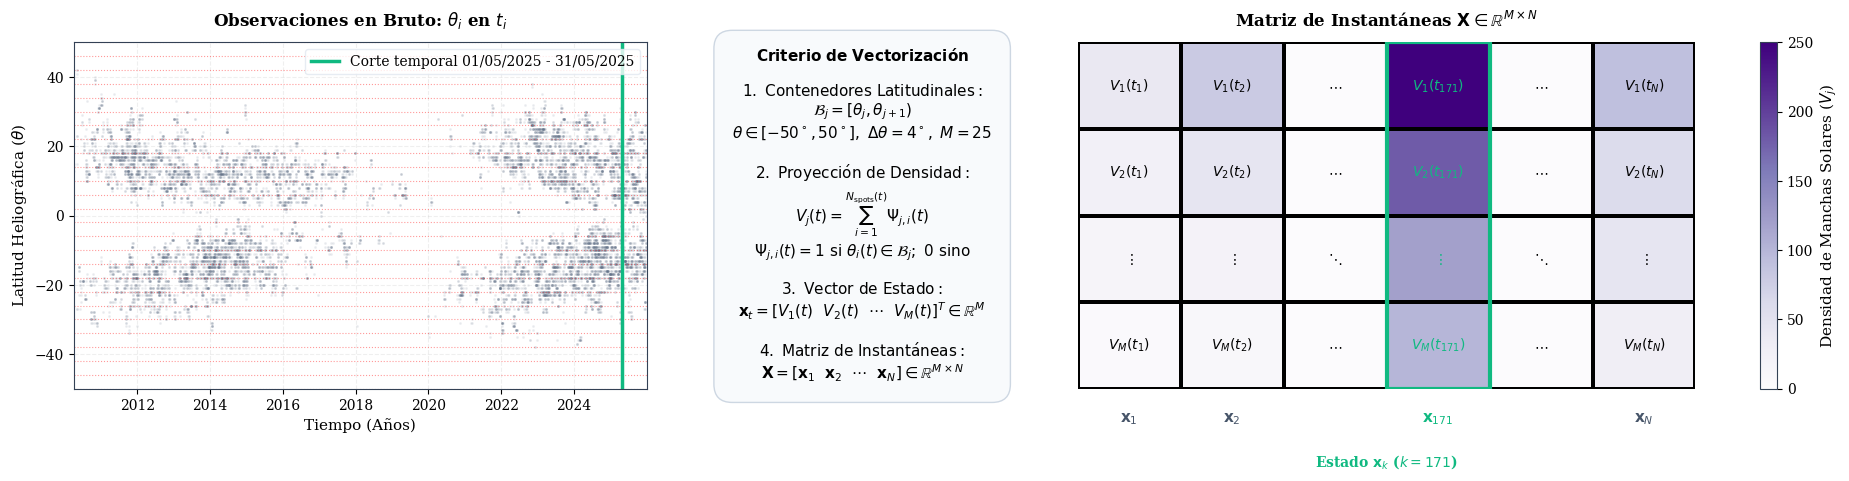
\includegraphics[width=1.04\linewidth, height=0.76\textheight, keepaspectratio]{dmd/discretizacion.png}}\par
    
    \vspace{0.03cm}
    {\scriptsize
    $\mathbf{X} \in \mathbb{R}^{M \times N} \xrightarrow{\text{SVD}} \mathbf{U}_r \mathbf{\Sigma}_r \mathbf{V}_r^T \implies \mathbf{x}_{k+1} = \mathbf{A}\mathbf{x}_k, \quad \tilde{\mathbf{A}} = \mathbf{U}_r^T \mathbf{X}' \mathbf{V}_r \mathbf{\Sigma}_r^{-1} \in \mathbb{R}^{r \times r}$ ($r \ll M$) [6].\par}
    
    \vfill
    {\raggedright\tiny\color{gray} [6] S. L. Brunton y J. N. Kutz, \textit{Dynamic Mode Decomposition: Data-Driven Modeling of Complex Systems}, SIAM, 2016.\par}
\end{frame}

\begin{frame}{Modelos de Deep Learning em Cascata \quad \setlength{\fboxrule}{1.2pt}\setlength{\fboxsep}{3pt}\raisebox{0.1ex}{\fcolorbox{llamativoMagenta}{white}{\scriptsize\textcolor{llamativoMagenta}{\textbf{Contribuição 4}}}}}
    \centering
    \vfill
    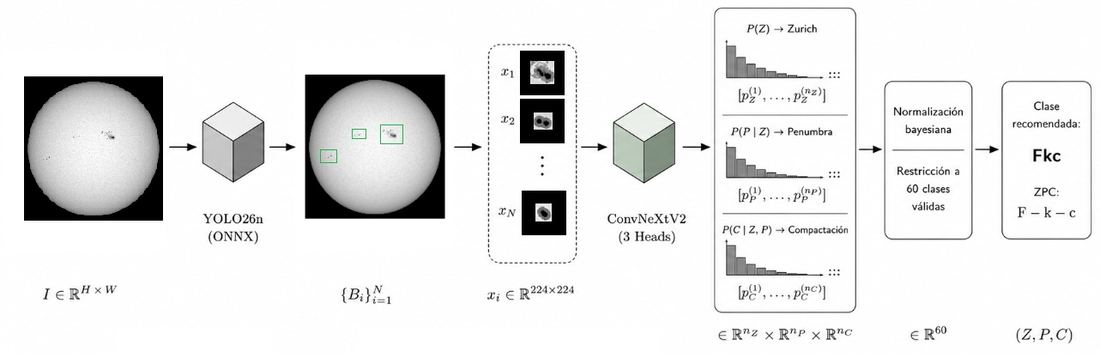
\includegraphics[height=0.74\textheight, width=0.98\linewidth, keepaspectratio]{sys/img_pipe.jpg}\par
    \vspace{0.08cm}
    {\scriptsize Pipeline hierárquico modular: Aquisição, detecção com YOLO e classificação morfológica com ConvNeXt.}
    \vfill
\end{frame}

\begin{frame}{Modelos de Deep Learning: Classificação Hierárquica e Normalização Bayesiana}
    \centering
    \vspace{-0.25cm}
    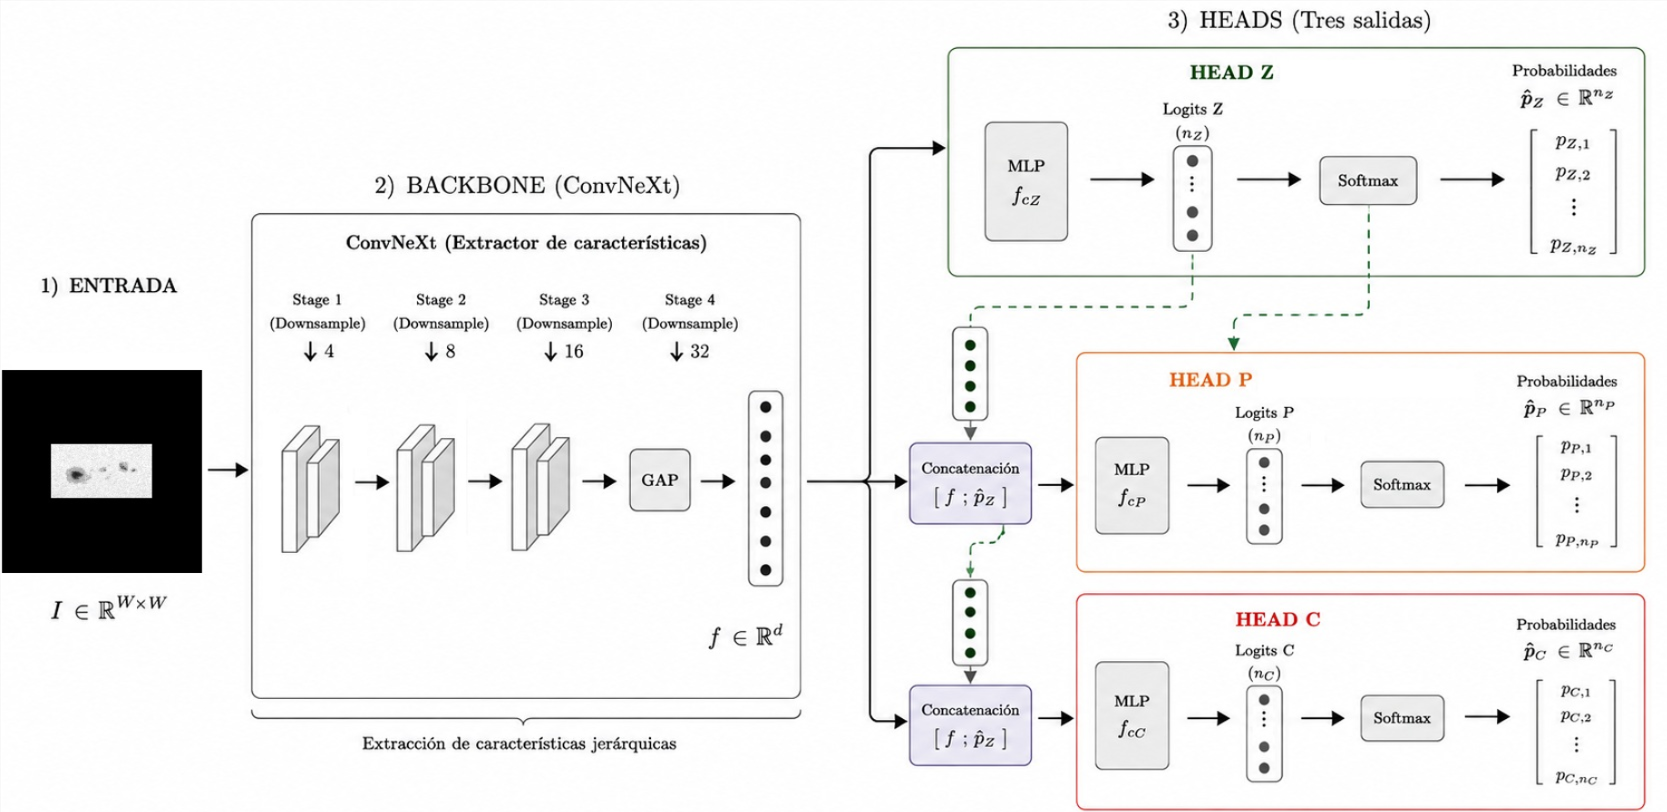
\includegraphics[width=\linewidth, height=0.69\textheight, keepaspectratio]{ml/convnext_arch.png}\par
    \vspace{0.06cm}
    
    \begin{minipage}{0.98\linewidth}
        \scriptsize
        Arquitetura multirrótulo ConvNeXt com três cabeças taxonômicas independentes $(Z, P, C)$ e restrição bayesiana $P(Z,P,C\mid x) \propto P(Z\mid x)P(P\mid x)P(C\mid x)\mathcal{M}_{ZPC}$, onde $\mathcal{M}_{ZPC} \in \{0,1\} \implies |\Omega_{\text{rec}}| = 60 \subset 168 = |\mathcal{Z} \times \mathcal{P} \times \mathcal{C}|$.
    \end{minipage}
\end{frame}

% \begin{frame}{Modelos de Deep Learning en Cascada: Entrenamiento de Arquitectura jerárquica ConvNeXtv2a}

%     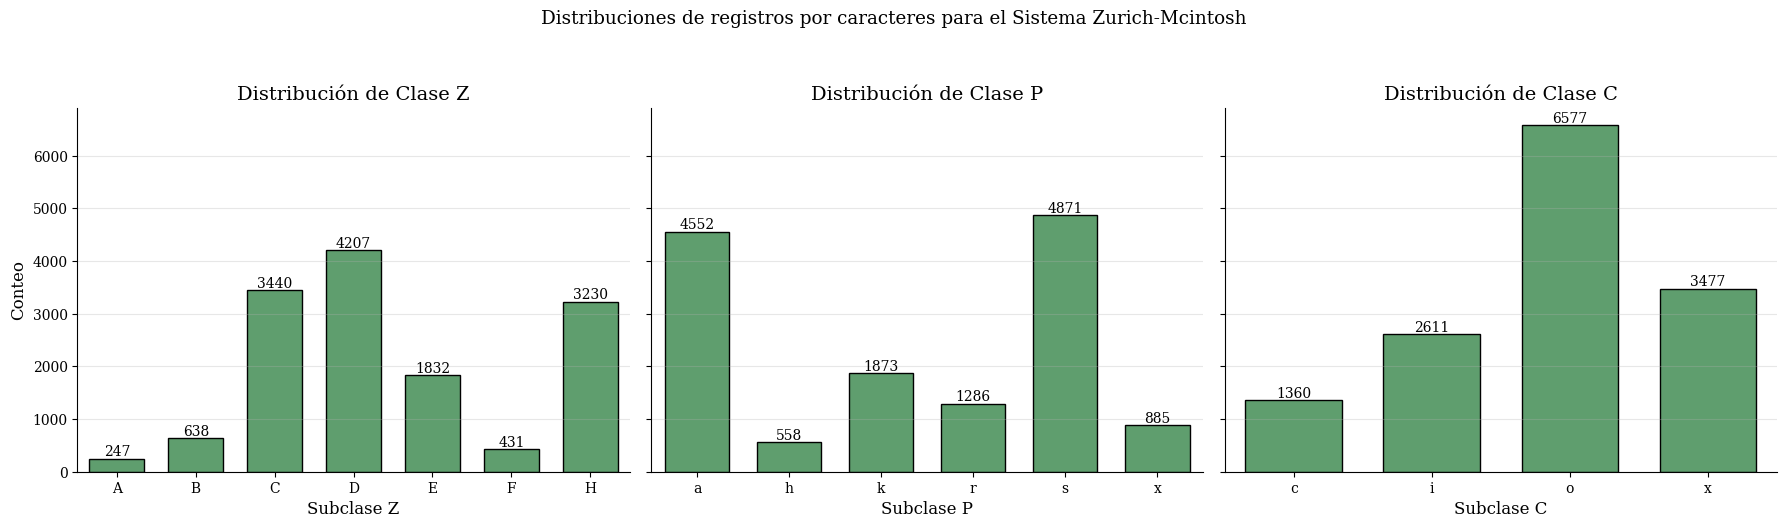
\includegraphics[height=0.62\textheight,width=0.96\linewidth,keepaspectratio]{data/char_hist.png}\par

%     \small
%     \begin{itemize}
%         \item Para mitigar el desbalance de clases se utilizaron \textbf{Class-Balanced Weights} basados en el \textit{Effective Number of Samples} [15].
%         \item Adem\'as, se incorpor\'o \textbf{remuestreo ponderado} mediante \textbf{\texttt{WeightedRandomSampler}}, reforzando la exposici\'on de clases minoritarias durante el entrenamiento.
%     \end{itemize}
    
%     \vfill
%     {\tiny\color{gray} [15] Y. Cui et al., “Class-balanced loss based on effective number of samples,” in Proc. IEEE/CVF CVPR, 2019, pp. 9268--9277.}
% \end{frame}

% \begin{frame}{Modelos de Deep Learning en Cascada: Entrenamiento de Arquitectura jerárquica ConvNeXtv2a}
%     \centering
%     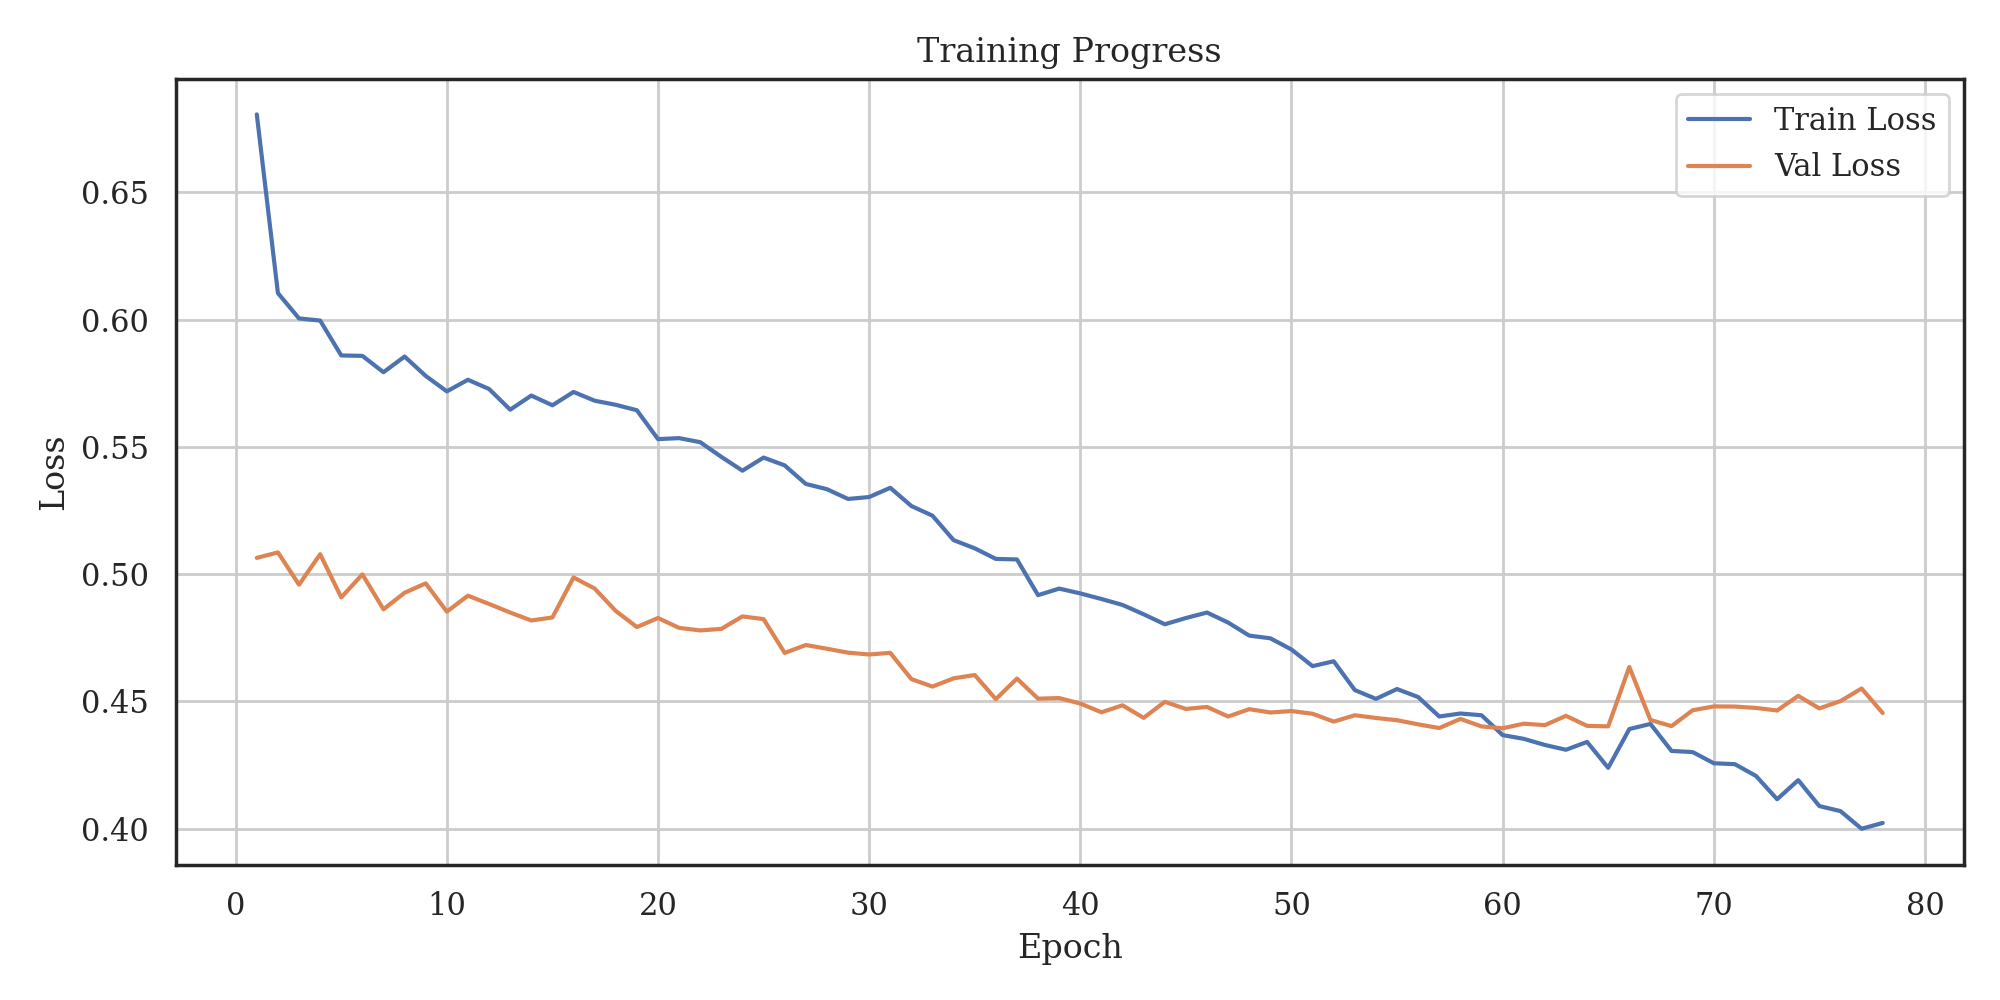
\includegraphics[height=0.78\textheight,width=0.96\linewidth,keepaspectratio]{ml/training_progress_classifier.png}
%     \vspace{0.08cm}
% \end{frame}

% \begin{frame}{Modelos de Deep Learning en Cascada: Entrenamiento de Arquitectura jerárquica ConvNeXtv2a}
%     \centering
%     \begin{columns}[T]
%         \begin{column}{0.4\linewidth}
%             \centering
%             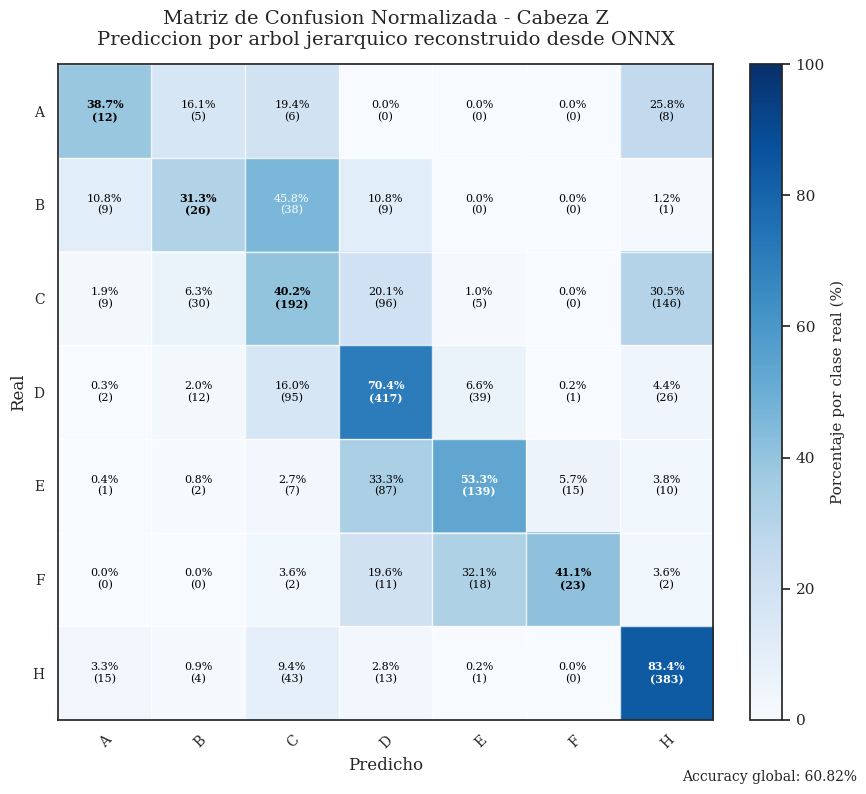
\includegraphics[width=\linewidth]{ml/conf_z.png}\par
%             {\tiny Matriz de confusión para Z.}
%         \end{column}
%         \begin{column}{0.4\linewidth}
%             \centering
%             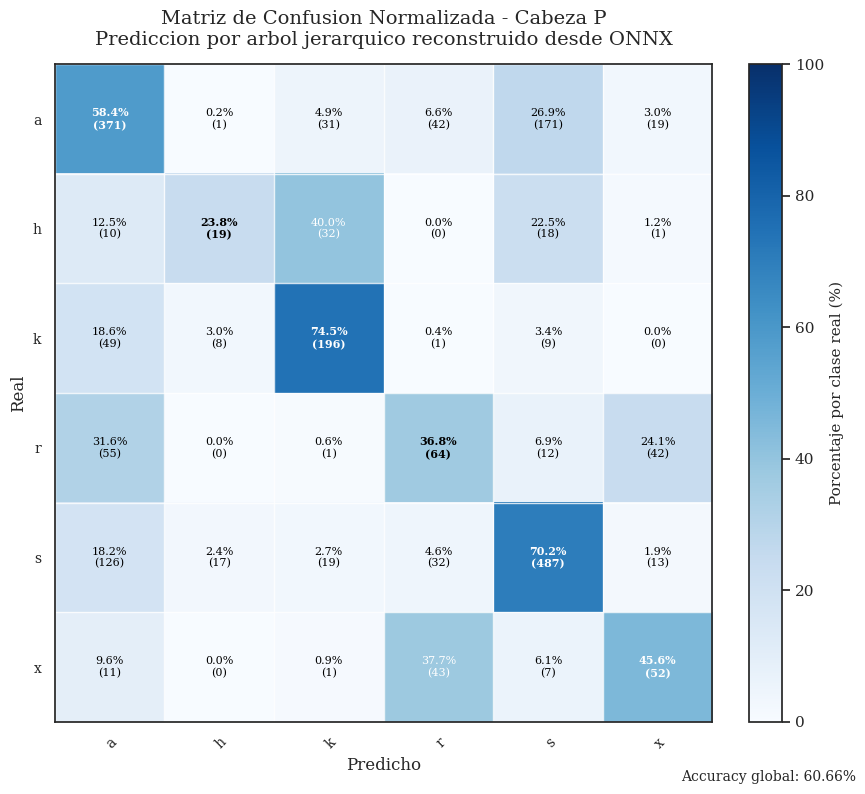
\includegraphics[width=\linewidth]{ml/conf_p.png}\par
%             {\tiny Matriz de confusión para P.}
%         \end{column}
%         \begin{column}{0.4\linewidth}
%             \centering
%             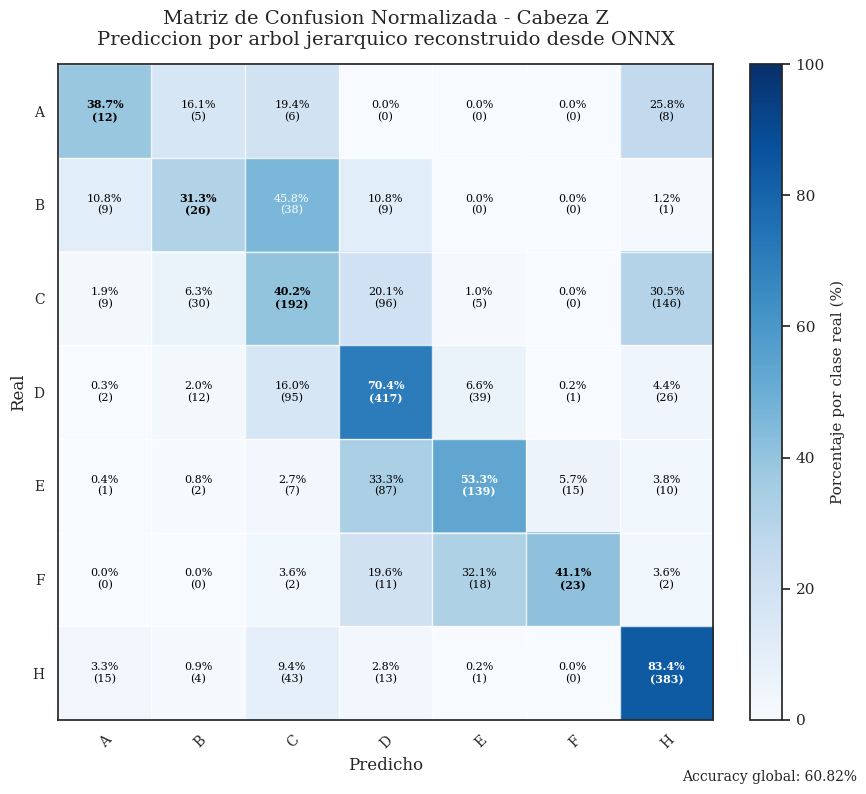
\includegraphics[width=\linewidth]{ml/conf_c.png}\par
%             {\tiny Matriz de confusión para C.}
%         \end{column}
%     \end{columns}
% \end{frame}

% \begin{frame}{Modelos de Deep Learning en Cascada: Formalismo de la normalización Bayesiana}
%     \centering
%     \small
%     \begin{align*}
%         P(Z,P,C\mid x)&=P(Z\mid x)P(P\mid Z,x)P(C\mid Z,P,x),\\
%         P_{\mathrm{base}}(Z,P,C\mid x)&=P(Z\mid x)P(P\mid x)P(C\mid x),\\
%         P_{\mathrm{rec}}(Z,P,C\mid x)&=
%         \frac{P_{\mathrm{base}}(Z,P,C\mid x)M_{ZPC}}
%         {\sum_{z,p,c}P_{\mathrm{base}}(z,p,c\mid x)M_{zpc}}.
%     \end{align*}
%     \begin{equation*}
%         (Z^\ast,P^\ast,C^\ast)=\arg\max_{Z,P,C}P_{\mathrm{rec}}(Z,P,C\mid x).
%     \end{equation*}\par
%     \vspace{0.05cm}
%     {\footnotesize La máscara $M_{ZPC}$ anula combinaciones no admisibles de la taxonomía, es decir $\{ \# Z \} \cdot \{ \# P \} \cdot \{ \# C \} = 7 \times 6 \times 4 = 168$ a las $60$ clases validas.}
% \end{frame}

% \begin{frame}{Modelos de Deep Learning en Cascada: Árbol de recomendaciones semánticas}
%     \centering
%     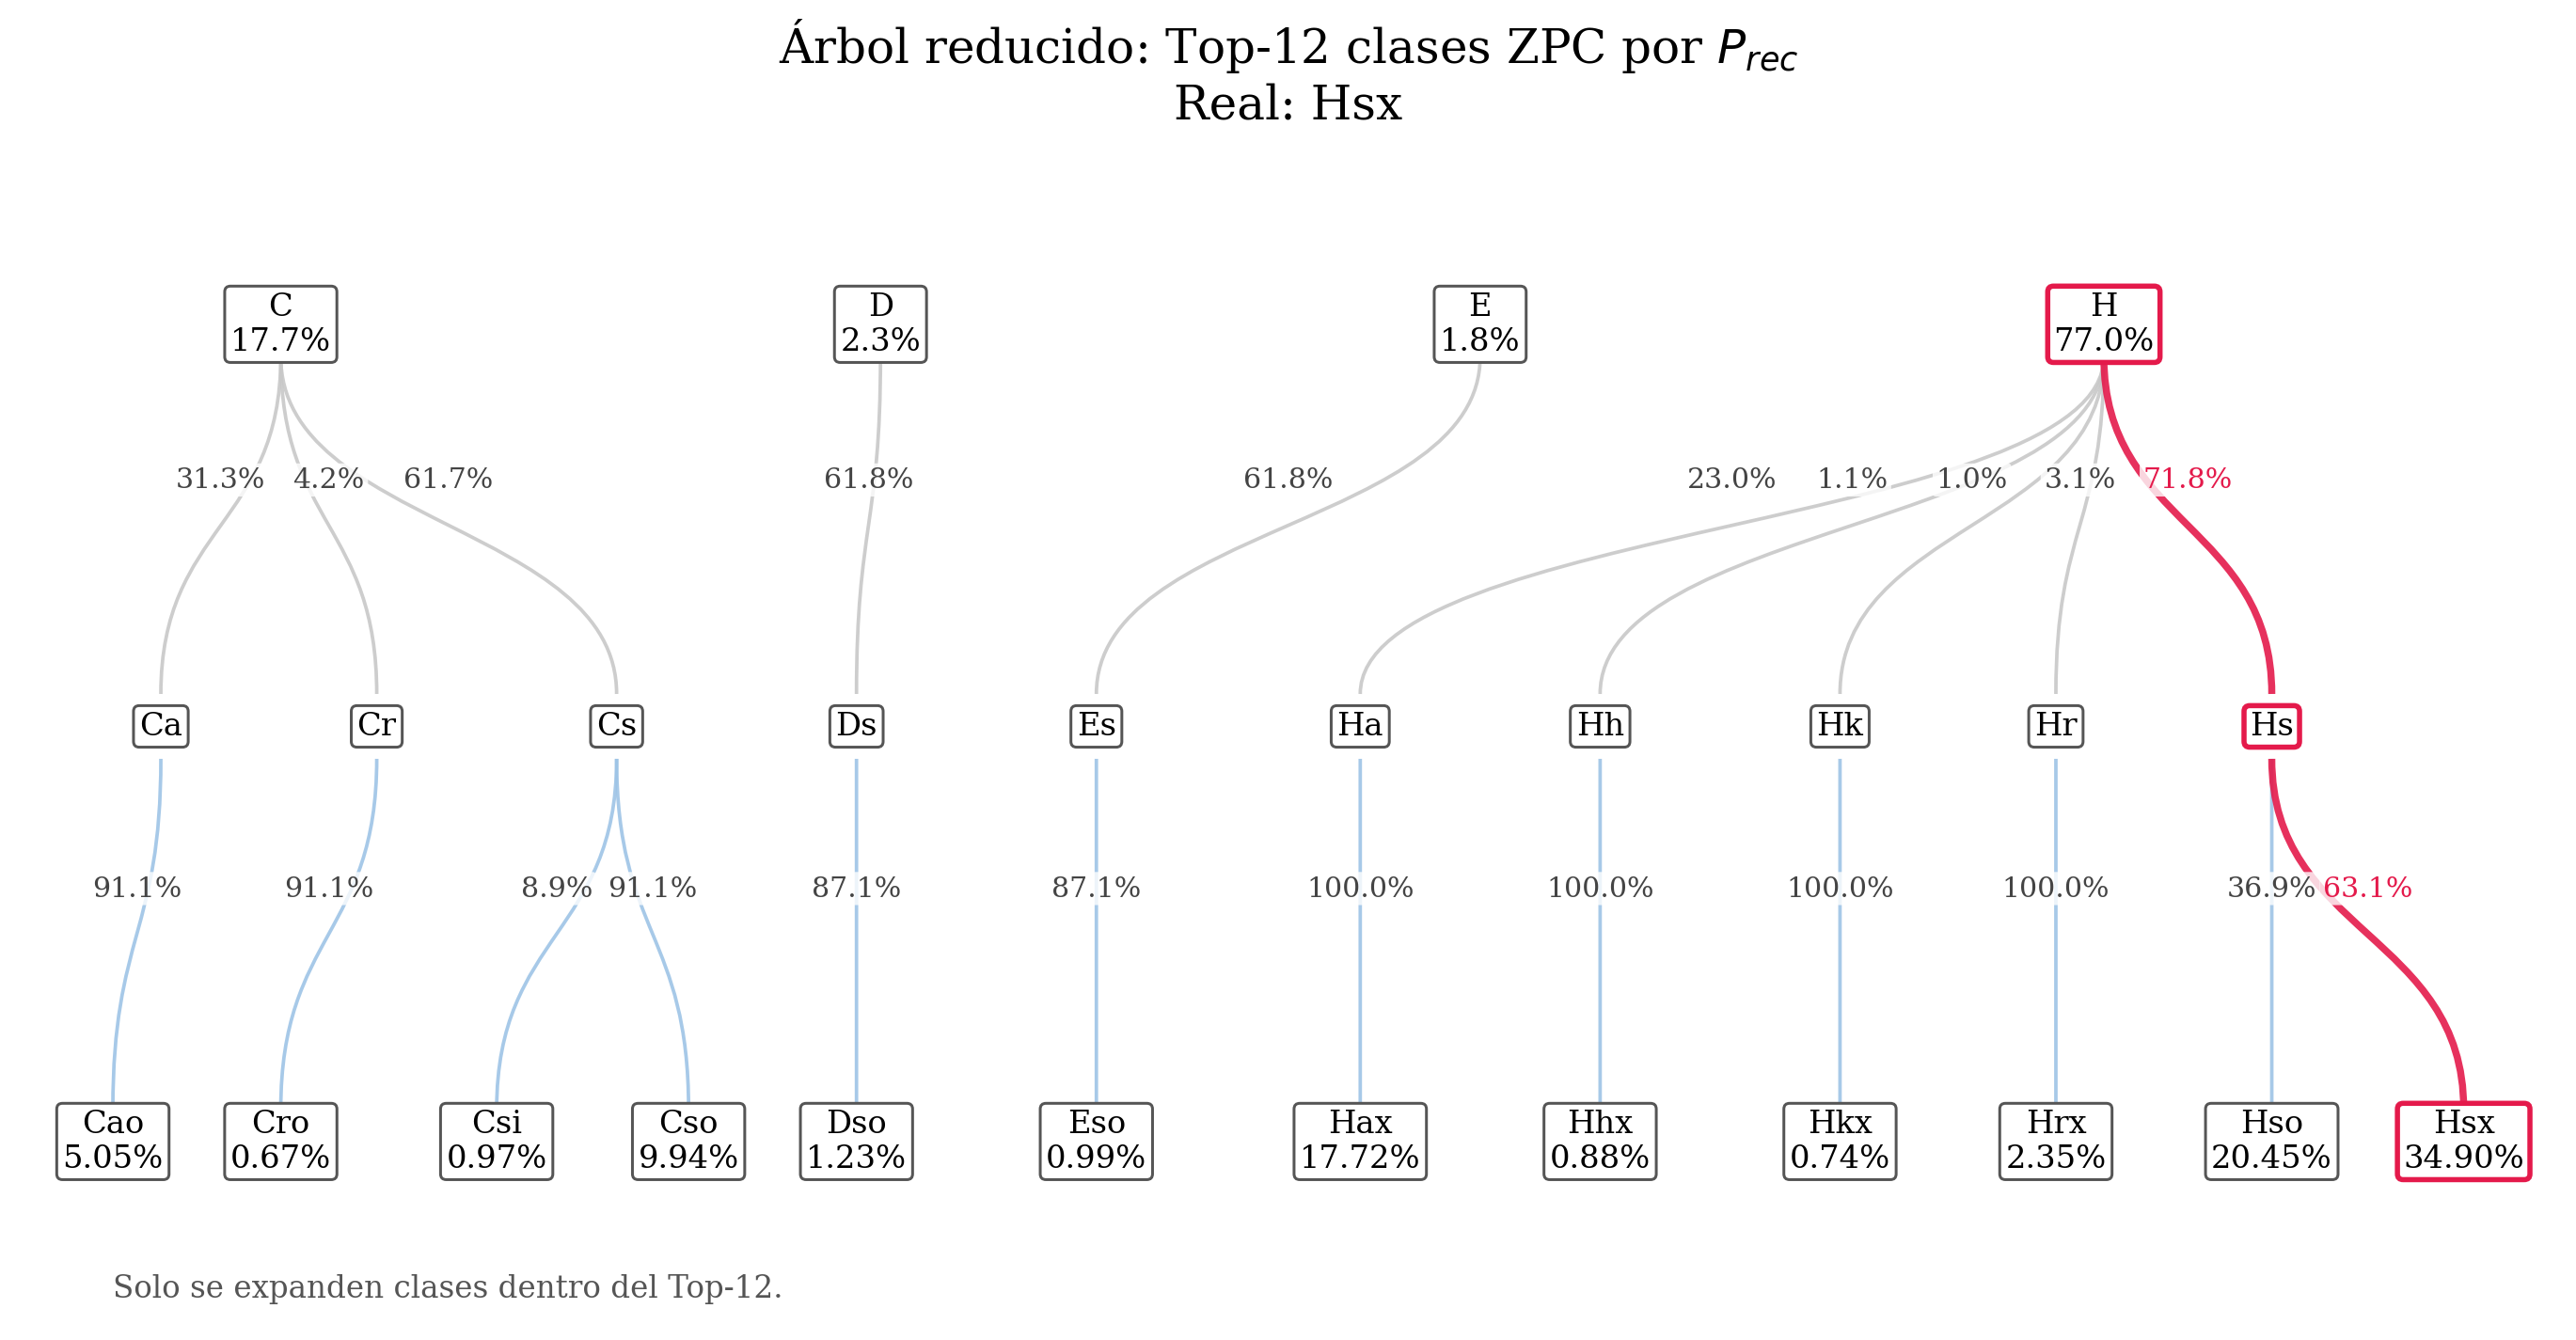
\includegraphics[height=0.85\textheight,width=0.96\linewidth,keepaspectratio]{ml/top12_tree.png}
%     \vspace{0.08cm}
% \end{frame}

% \begin{frame}{Modelos de Deep Learning en Cascada: Recomendaciones semánticas}
%     \centering
%     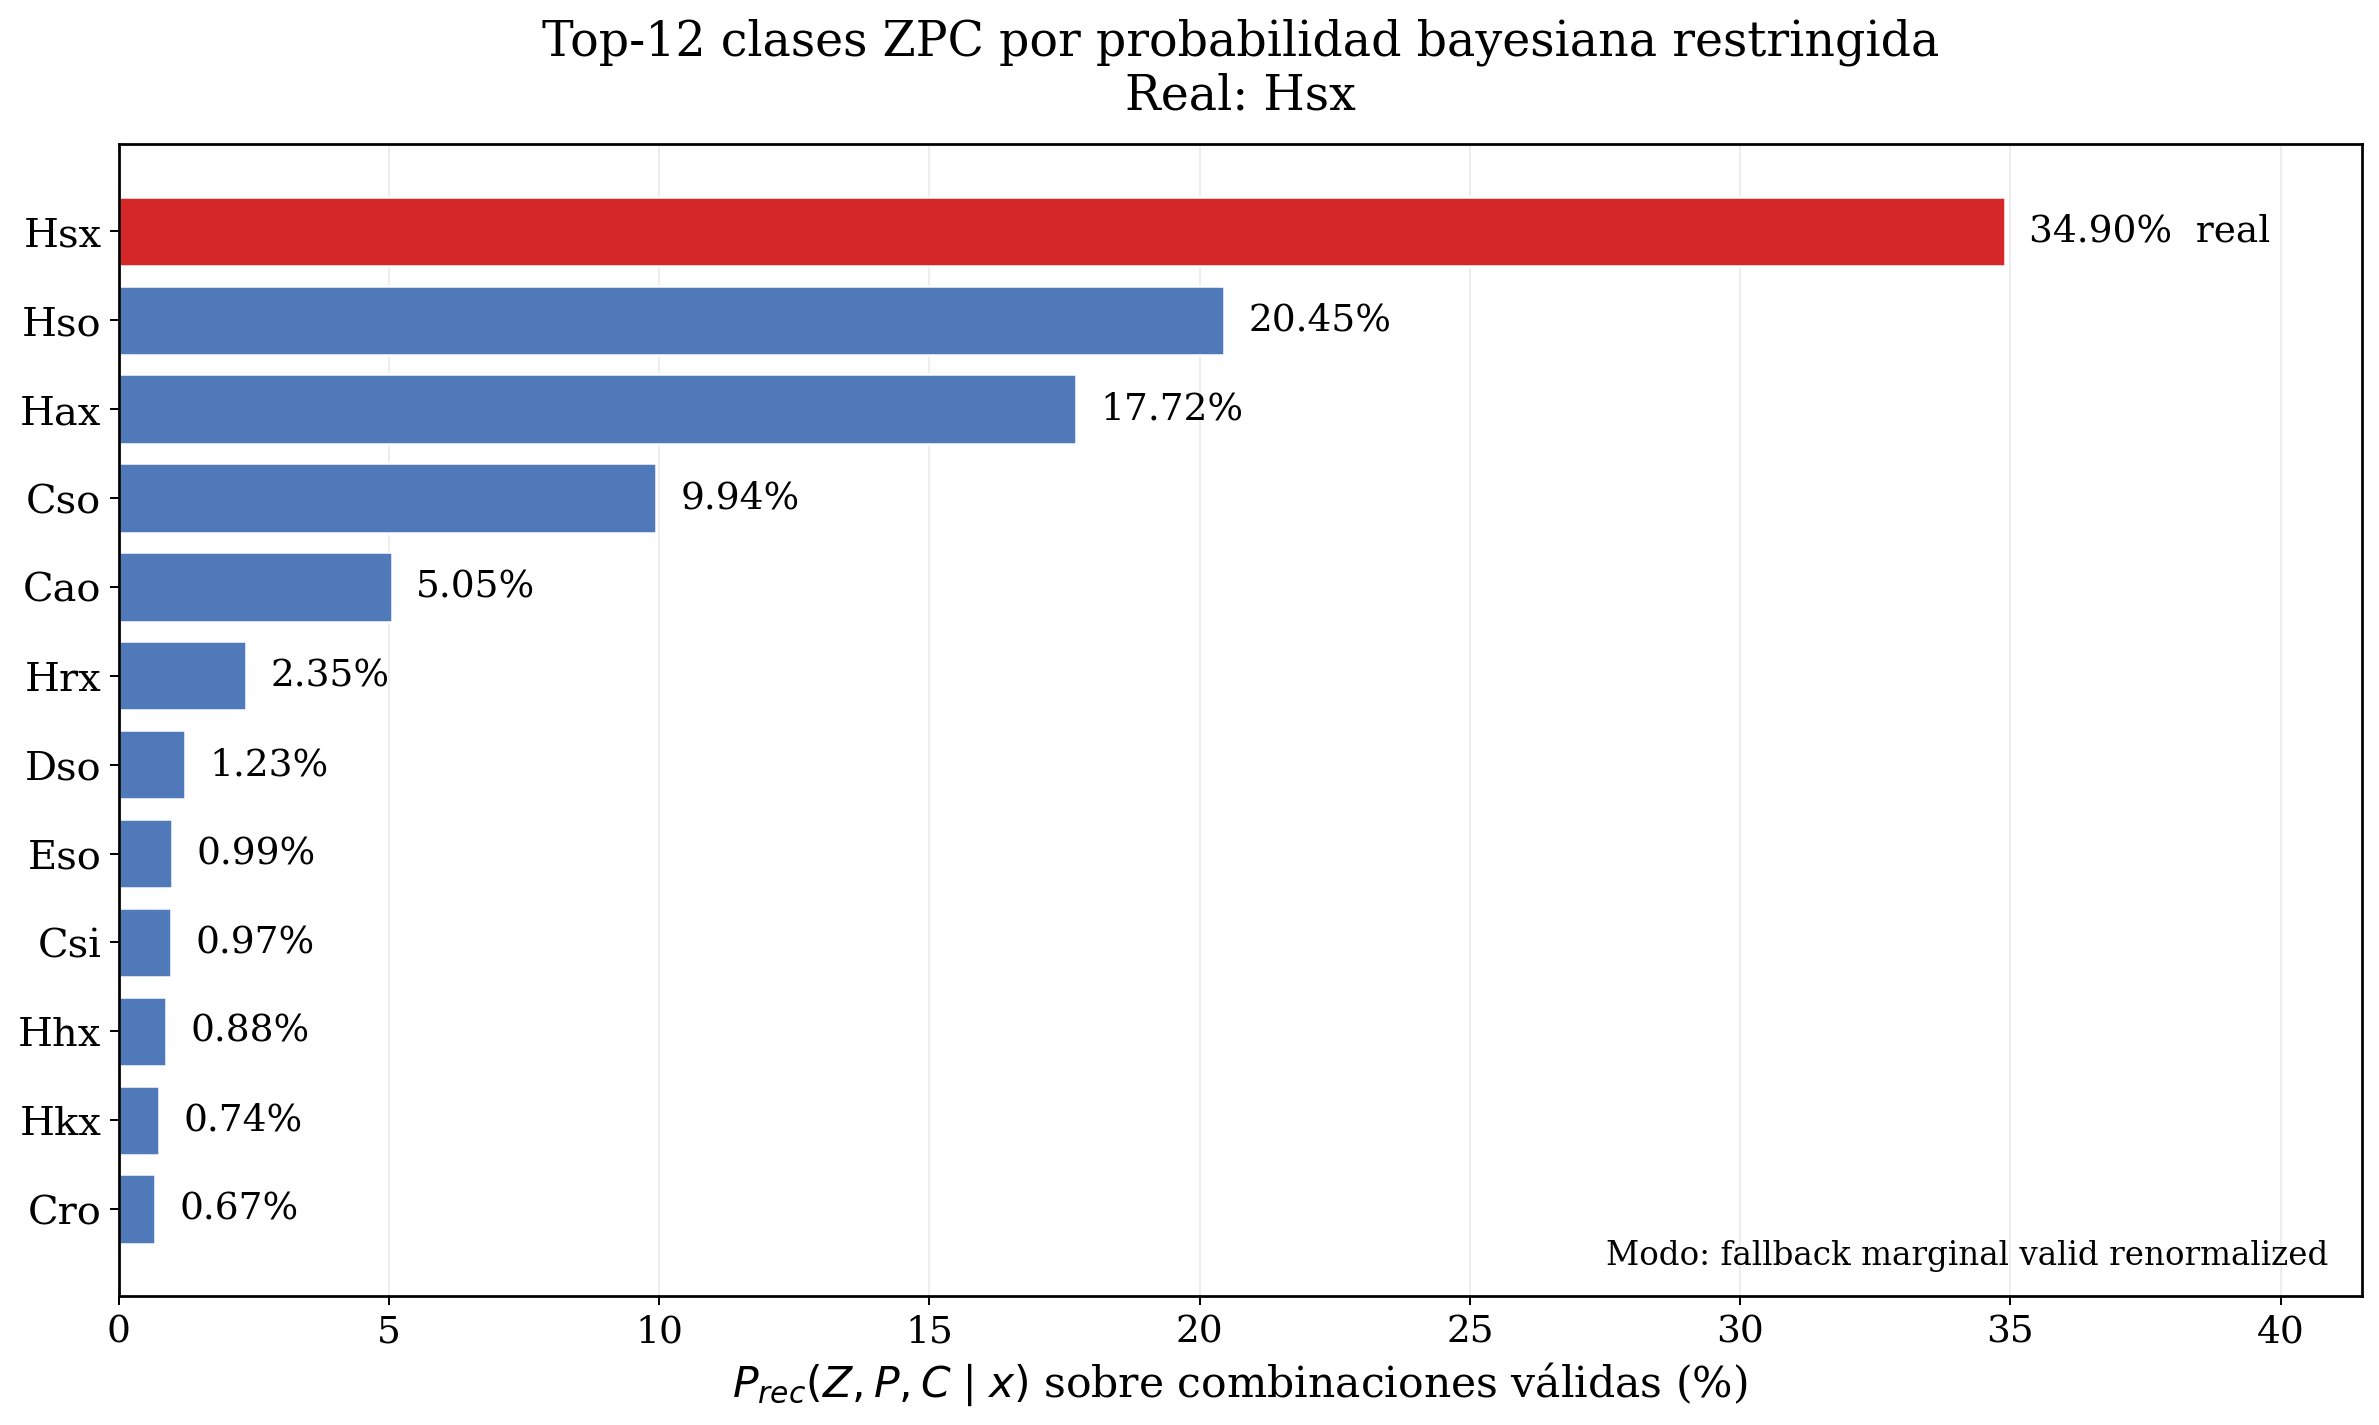
\includegraphics[height=0.82\textheight,width=0.96\linewidth,keepaspectratio]{ml/top12_rec.png}
%     \vspace{0.08cm}
% \end{frame}



% \begin{frame}{Estructura de Base de Datos (Supabase)}
%     \centering
%     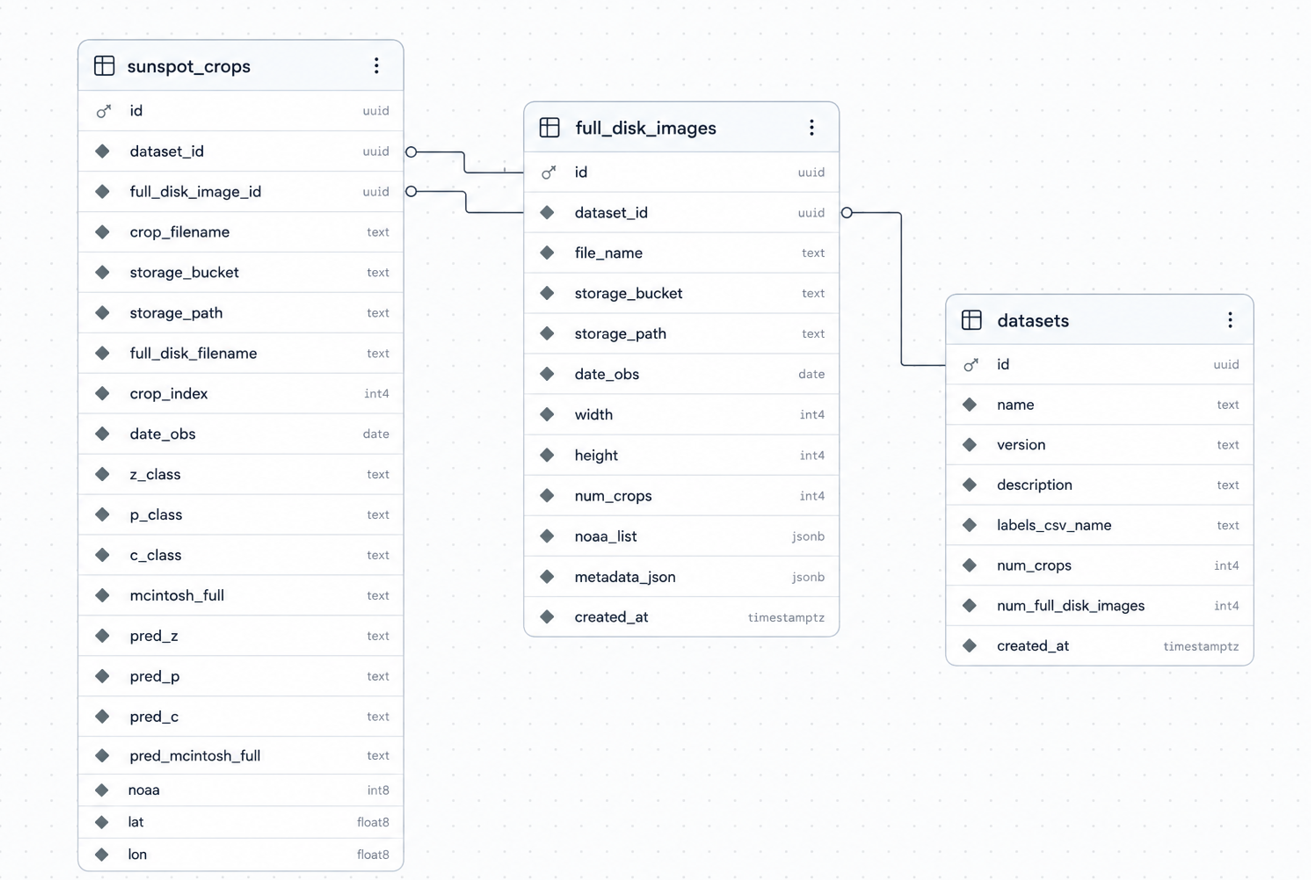
\includegraphics[height=0.82\textheight,width=0.96\linewidth,keepaspectratio]{data/db_schema.png}
%     \vspace{0.08cm}
% \end{frame}

% \begin{frame}{Plataforma Web: Inicio \quad \setlength{\fboxrule}{1.2pt}\setlength{\fboxsep}{3pt}\raisebox{0.1ex}{\fcolorbox{llamativoMagenta}{white}{\scriptsize\textcolor{llamativoMagenta}{\textbf{Contribución 5}}}}}
    
%     % --- CONTENIDO PRINCIPAL ---
%     \centering
%     \vfill
%     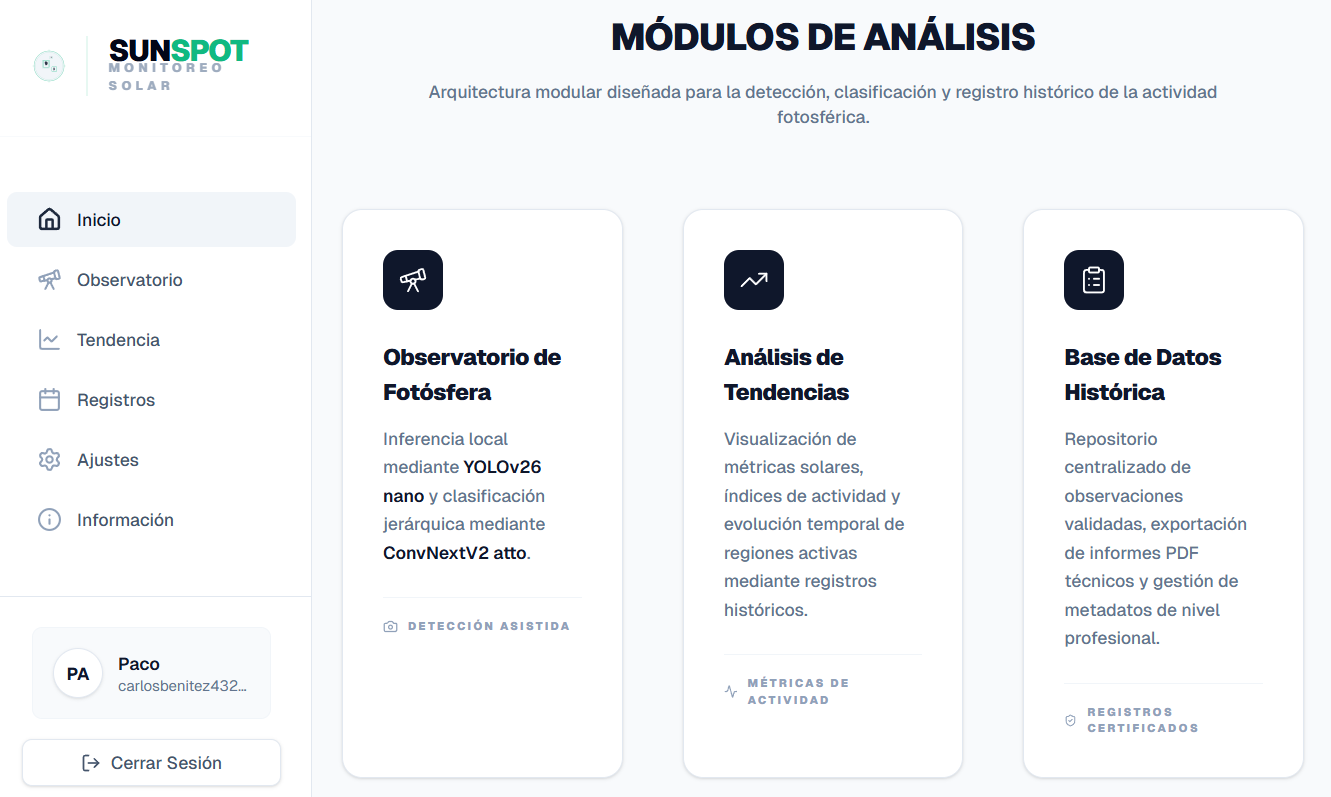
\includegraphics[height=0.82\textheight, width=0.98\linewidth, keepaspectratio]{web/home.png}
%     \vfill
    
% \end{frame}

% \begin{frame}{Plataforma Web: Carga de imagen}
    
%     % --- CONTENIDO PRINCIPAL ---
%     \centering
%     \vfill
%     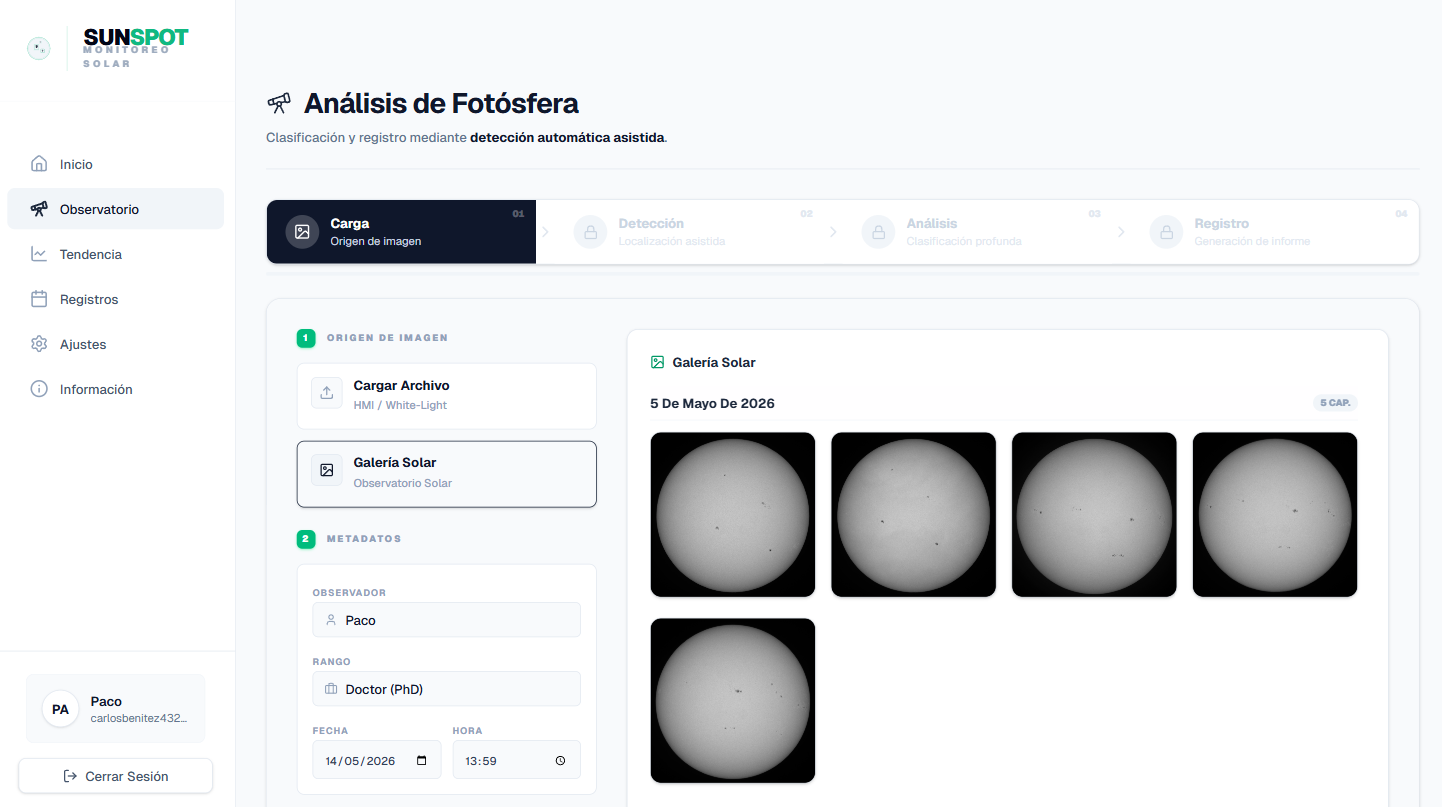
\includegraphics[height=0.82\textheight, width=0.98\linewidth, keepaspectratio]{web/upload.png}
%     \vfill
    
% \end{frame}

\section{Resultados}

\begin{frame}{Resultados: Modelos de Detecção e Classificação}
    \vspace{-0.1cm}

    % --- Estructura Principal en Dos Columnas Grandes ---
    \begin{columns}[c, onlytextwidth]
        
        % Columna IZQUIERDA: Imagen completa con su respectivo Caption
        \begin{column}{0.40\textwidth}
            \begin{figure}
                \centering
                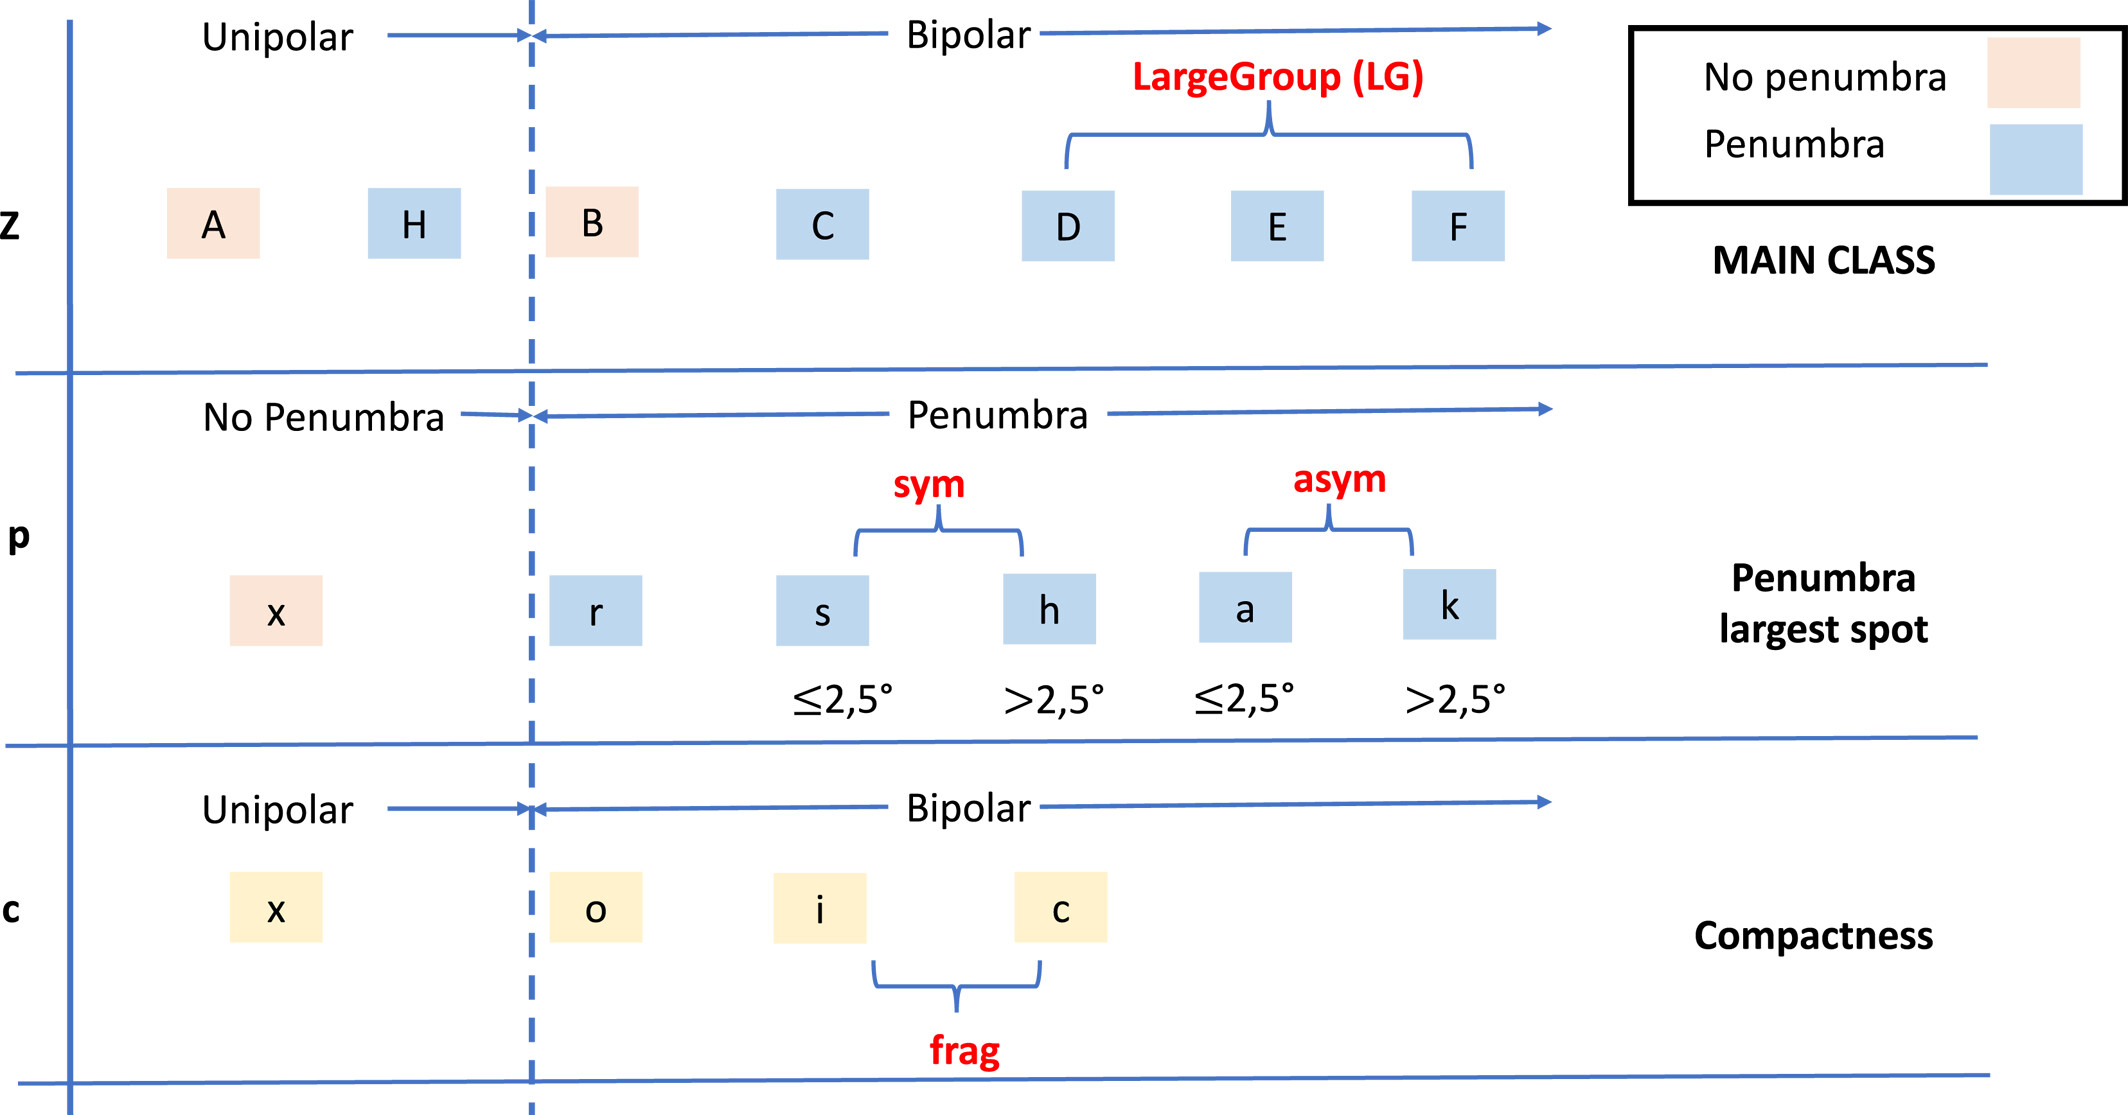
\includegraphics[height=0.58\textheight, width=\linewidth, keepaspectratio]{ref/sayezCompactacion.jpg}\par
                \vspace{0.05cm}
                {\scriptsize Compactação de classes em Sayez et al.}
            \end{figure}
        \end{column}
        
        \hfill
        
        % Columna DERECHA: Contiene la Tabla y justo debajo el Texto de Sayez
        \begin{column}{0.58\textwidth}
            \centering
            
            % 1. Tabla Comparativa Escalada y Compacta
            \renewcommand{\arraystretch}{1.1}
            \setlength{\tabcolsep}{4pt} 
            \begin{table}
                \scriptsize
                \centering
                \begin{tabular}{lcccc}
                    \toprule
                    \textbf{Autor} & \textbf{F1-Z} & \textbf{F1-P} & \textbf{F1-C} & \textbf{F1 p.} \\
                    \midrule
                    Palladino (2022) [7] & \textcolor{red!80!black}{\textbf{0.67}} & \textcolor{green!70!black}{0.55} & \textcolor{red!80!black}{\textbf{0.72}} & \textcolor{green!70!black}{0.65} \\
                    Sayez (2023) [8] & \textcolor{red!80!black}{\textbf{0.68}} & \textcolor{red!80!black}{\textbf{0.65}} & \textcolor{red!80!black}{\textbf{0.72}} & \textcolor{red!80!black}{\textbf{0.68}} \\
                    Deng (2025) [9] & \textcolor{green!70!black}{0.47} & \textcolor{green!70!black}{0.41} & \textcolor{green!70!black}{0.60} & \textcolor{green!70!black}{0.49} \\
                    
                    % Fila de la propuesta con celdas pintadas en azul institucional y texto en blanco para alto contraste
                    \cellcolor{azulPropuesta}\textcolor{white}{\textbf{Proposta}} & 
                    \cellcolor{azulPropuesta}\textcolor{white}{\textbf{0.65}} & 
                    \cellcolor{azulPropuesta}\textcolor{white}{\textbf{0.63}} & 
                    \cellcolor{azulPropuesta}\textcolor{white}{\textbf{0.71}} & 
                    \cellcolor{azulPropuesta}\textcolor{white}{\textbf{0.66}} \\
                    \bottomrule
                \end{tabular}
            \end{table}

            \vspace{0.15cm}

            \scriptsize
            Sayez et al. (2023) [8] agrupa as classes de alguns caracteres, de modo que é esperada uma melhoria nas métricas; contudo, esse ajuste rompe a operacionalidade do modelo ao introduzir uma taxonomia distinta.
            
        \end{column}
        
    \end{columns}

    \vfill

    % --- Bloque de Referencias Unificado y Compacto ---
    {\raggedright\tiny\color{gray}
    [7] L. Palladino, E. Ntagiou, J. Klug, J. Palacios, y R. Keil, “Sunspot groups detection and classification on SDO/HMI images using deep learning techniques,” in 2022 IEEE Aerospace Conference. IEEE, 2022, pp. 1–10. \par\vspace{0.03cm}
    [8] M. Sayez et al., “SunSCC: Automated solar classification dataset,” Astronomy \& Astrophysics, 2023. \par\vspace{0.03cm}
    [9] X. Deng et al., “Deep learning-based McIntosh classification of sunspotgroups,” Astronomy and Computing, vol. 53, p. 100995, 2025.\par}
\end{frame}

\begin{frame}{Resultados: Modelos Preditivos}
    \centering
    \vspace{0.08cm}
    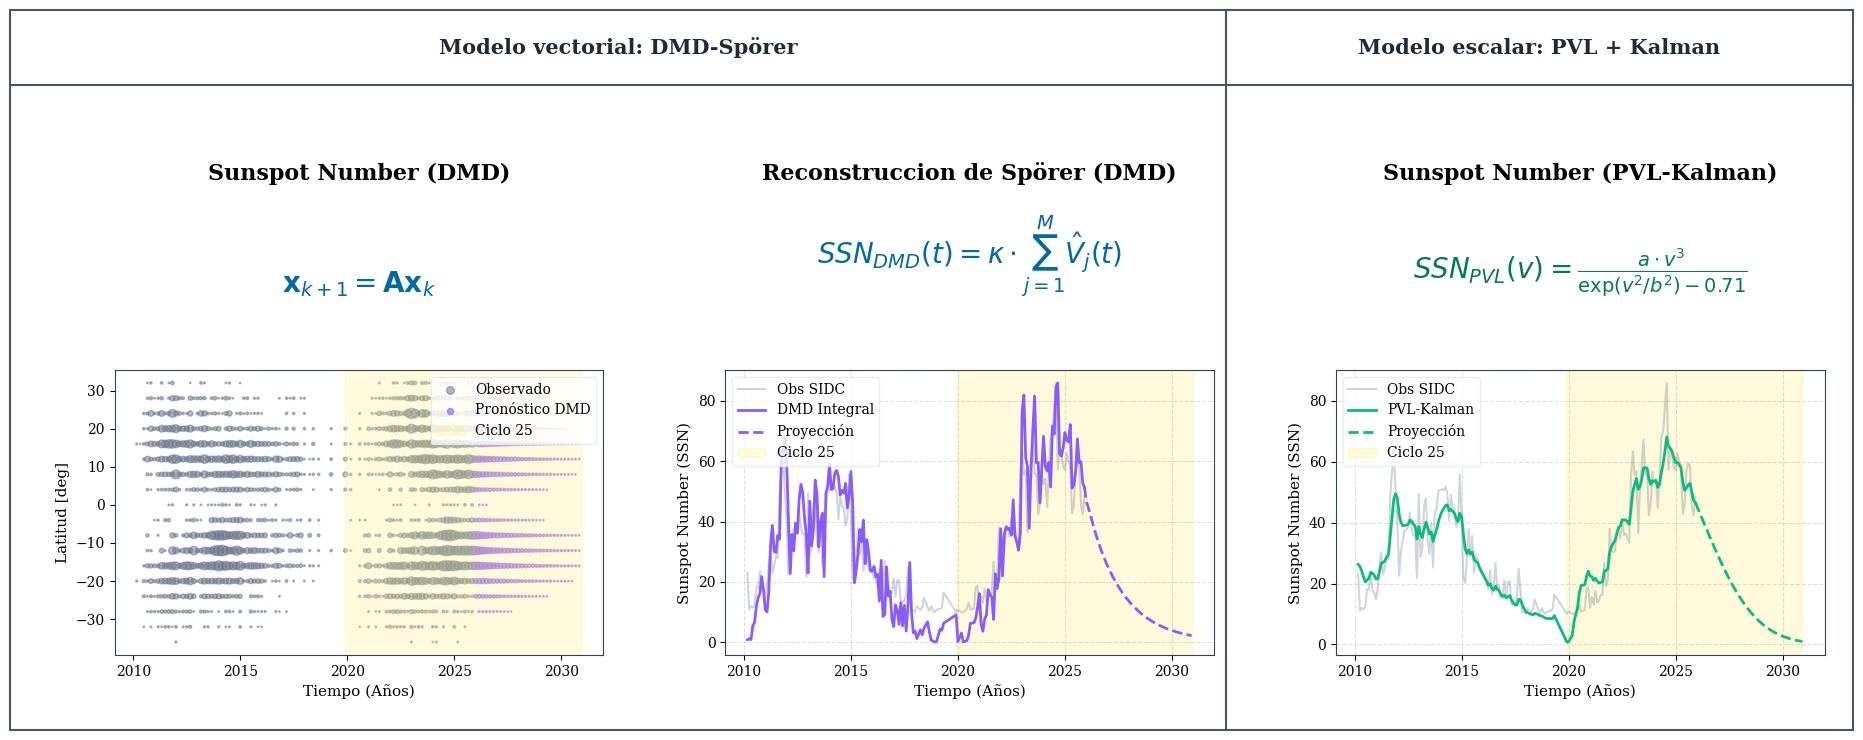
\includegraphics[width=\linewidth, height=0.52\textheight, keepaspectratio]{dmd/model_results.png}\par
    \vspace{0.05cm}
    
    \renewcommand{\arraystretch}{1.08}
    \setlength{\tabcolsep}{10pt}
    \begin{table}
        \scriptsize
        \centering
        \begin{tabular}{lcccc}
            \toprule
            \textbf{Modelo} & \textbf{MAE} & \textbf{RMSE} & \textbf{MAPE} & $\mathbf{R^2}$ \\
            \midrule
            PVLK [10] & 15.31 & 22.02 & 33.27\% & 0.8173 \\
            \cellcolor{azulPropuesta}\textcolor{white}{\textbf{DMD (Proposta)}} & 
            \cellcolor{azulPropuesta}\textcolor{white}{\textbf{15.22}} & 
            \cellcolor{azulPropuesta}\textcolor{white}{\textbf{20.30}} & 
            \cellcolor{azulPropuesta}\textcolor{white}{\textbf{32.54\%}} & 
            \cellcolor{azulPropuesta}\textcolor{white}{\textbf{0.8449}} \\
            \bottomrule
        \end{tabular}
    \end{table}

    \vfill
    {\raggedright\tiny\color{gray}
    [10] T. Podladchikova y R. Van der Linden, “Kalman filter technique for improving prediction of smoothed monthly sunspot numbers,” \textit{Solar Physics}, vol. 271, no. 2, pp. 469--485, 2011.\par}
\end{frame}

% \begin{frame}{Resultados: Adquisición y nodo local}
%     \small
%     \vspace{-0.1cm}
    
%     \begin{columns}[c] % <--- Centrado vertical global para las columnas
        
%         % COLUMNA IZQUIERDA: Imagen Dominante
%         \begin{column}[c]{0.55\textwidth} % <--- Centrado vertical individual
%             \centering
%             \textbf{Captura solar registrada el 2026-05-05}\\[0.1cm]
%             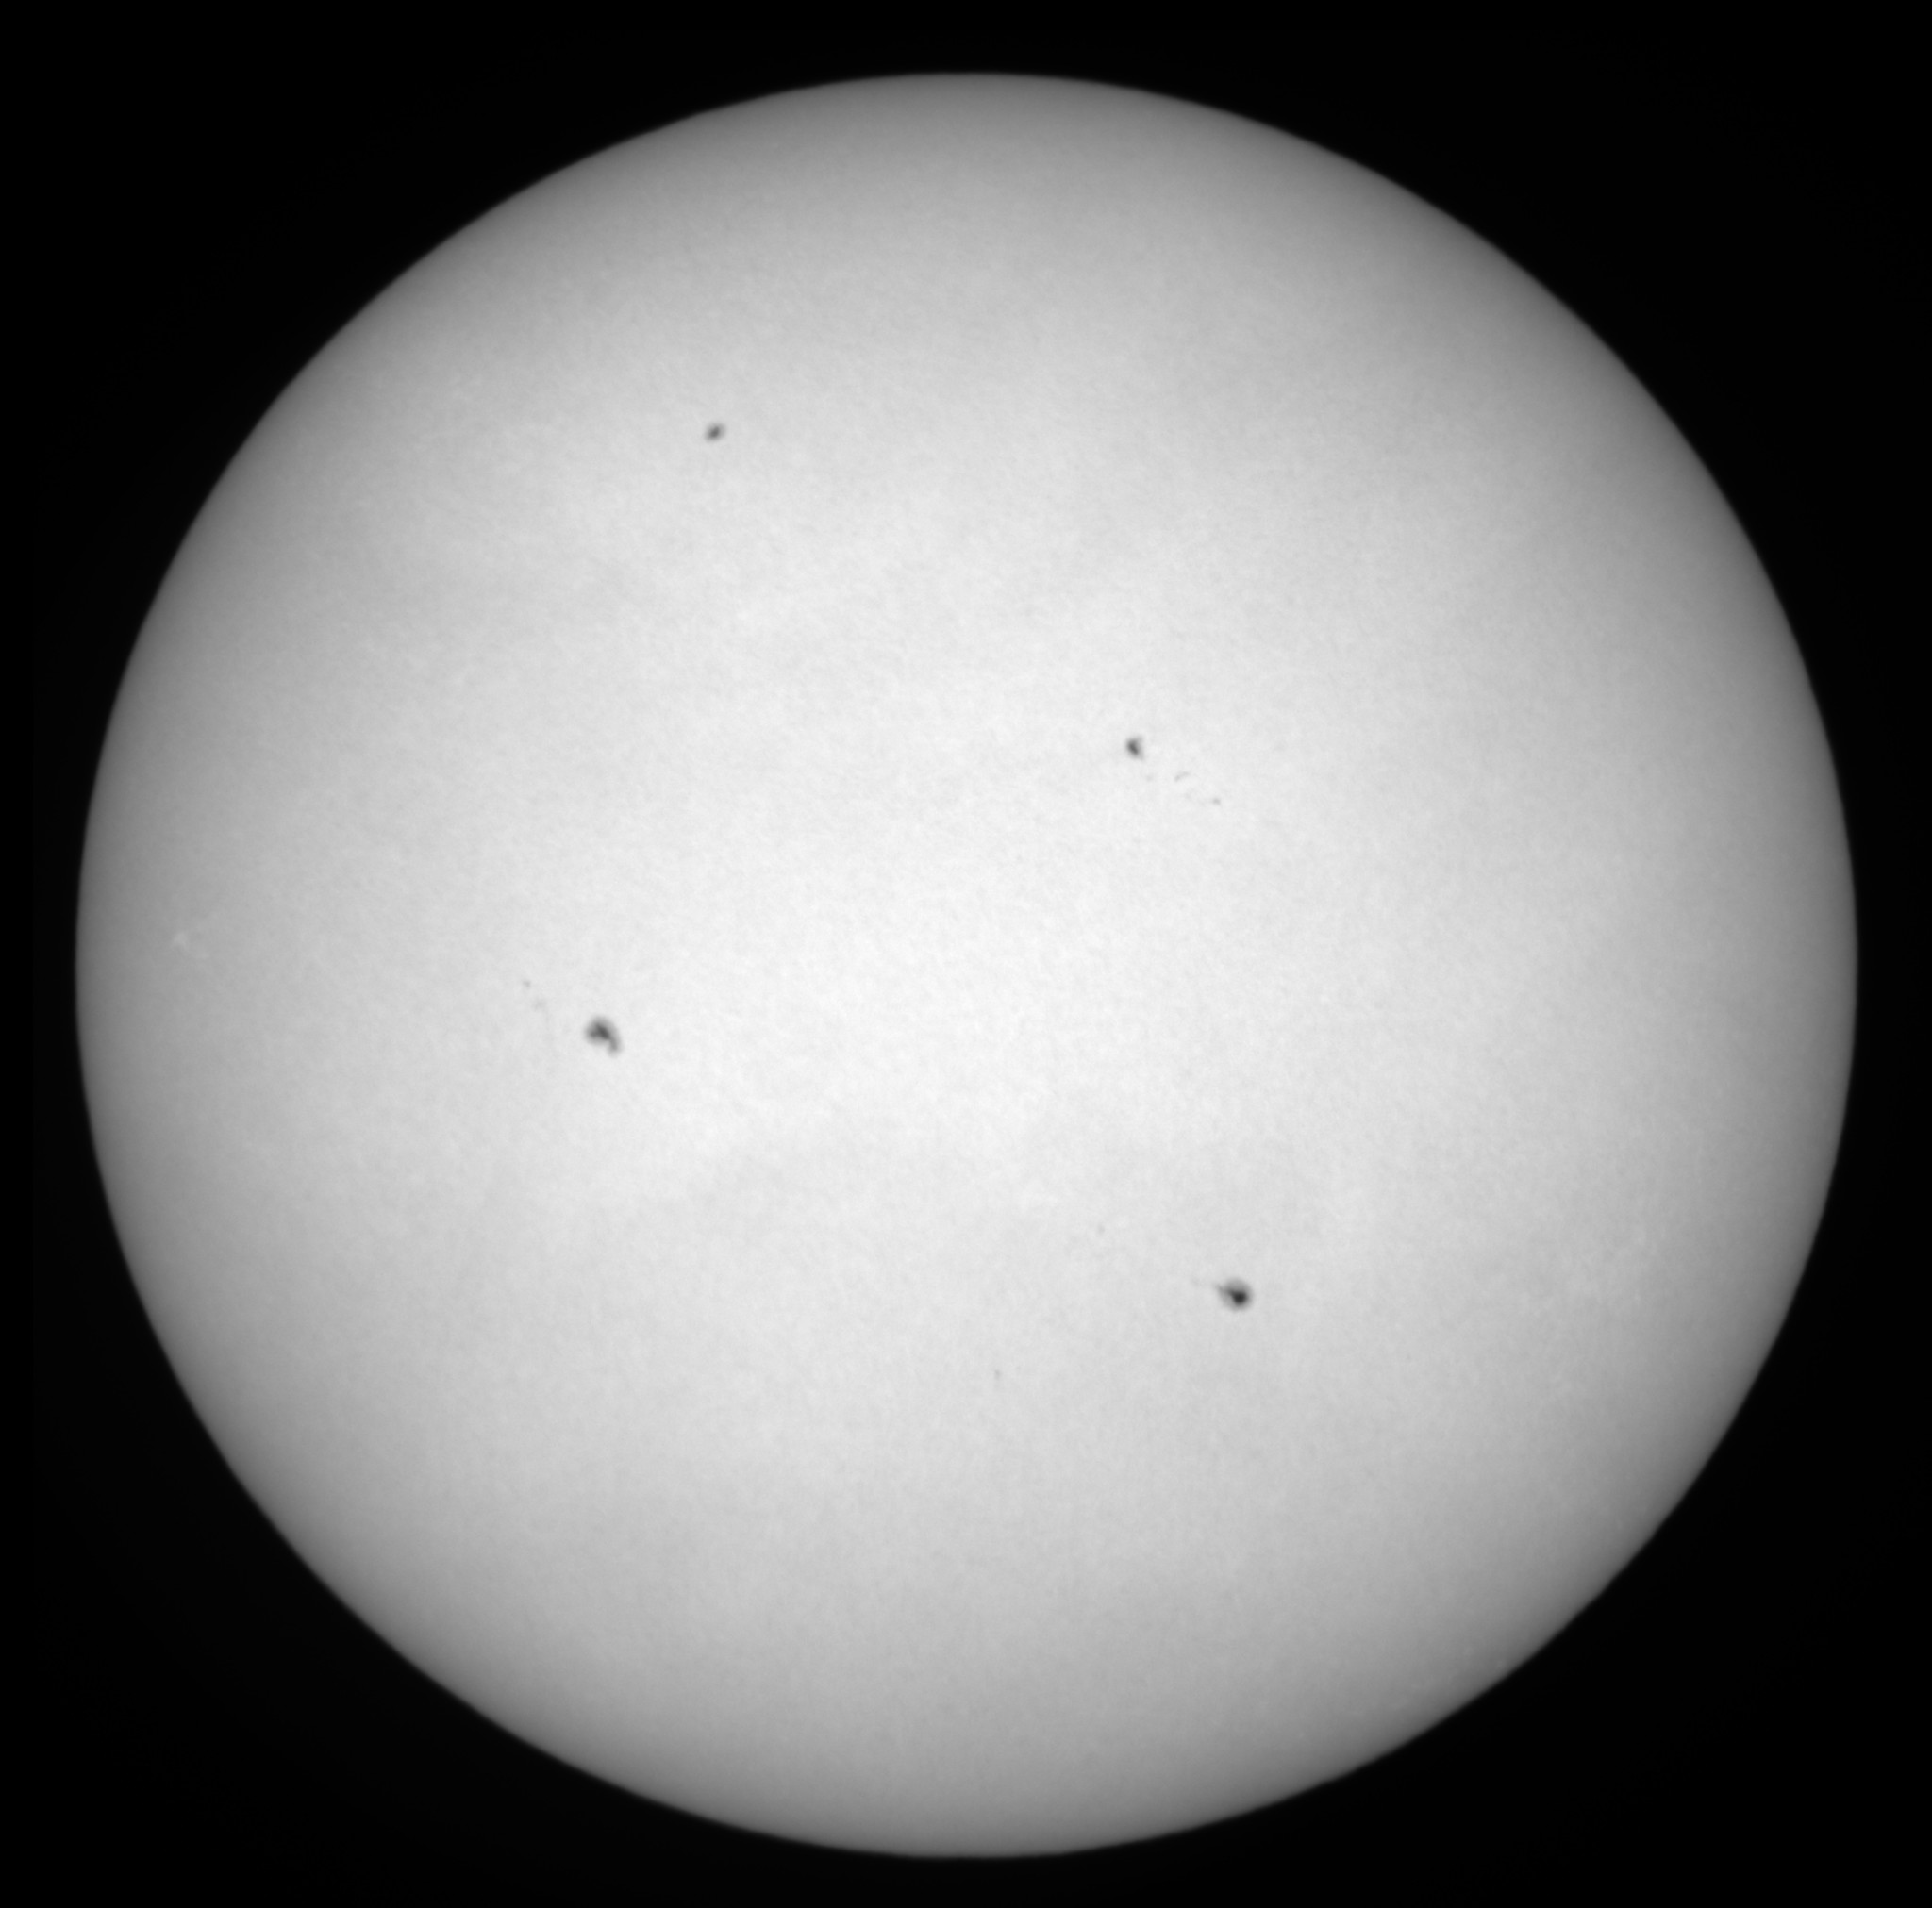
\includegraphics[width=0.95\textwidth, height=6.0cm, keepaspectratio]{obs/capture.jpg} 
%         \end{column}
        
%         % COLUMNA DERECHA: Ambas tablas centradas respecto a la imagen
%         \begin{column}[c]{0.42\textwidth} % <--- Centrado vertical individual
%             \centering
            
%             % Primera Tabla: Adquisición
%             \scriptsize \textbf{Adquisición}\\[0.05cm]
%             \renewcommand{\arraystretch}{1.0} 
%             \begin{tabular}{lc}
%                 \toprule
%                 \textbf{Parámetro} & \textbf{Valor} \\
%                 \midrule
%                 Formato & FITS / RGB24 \\
%                 Resolución & 1936 $\times$ 1216 px \\
%                 FPS / Exposición & 15 / 500 $\mu$s \\
%                 \bottomrule
%             \end{tabular}
            
%             \vspace{0.4cm} % Un toque más de separación para balancear el bloque
            
%             % Segunda Tabla: Raspberry Pi 5
%             \textbf{Raspberry Pi 5}\\[0.05cm]
%             \begin{tabular}{lc}
%                 \toprule
%                 \textbf{Métrica} & \textbf{Valor} \\
%                 \midrule
%                 Captura + Guardado & 600 ms \\
%                 Preprocesamiento & 1350 ms \\
%                 Sincronización & 3800 ms/img \\
%                 CPU medio/máx. & 38\% / 72\% \\
%                 RAM / Temp. 25 min & 3.3 GB / 57 $^{\circ}$C \\
%                 \bottomrule
%             \end{tabular}
%         \end{column}
        
%     \end{columns}
% \end{frame}


% \begin{frame}{Resultado de Campo: Plataforma Web (Detección con YOLO26n ONNX)}
%     \centering
%     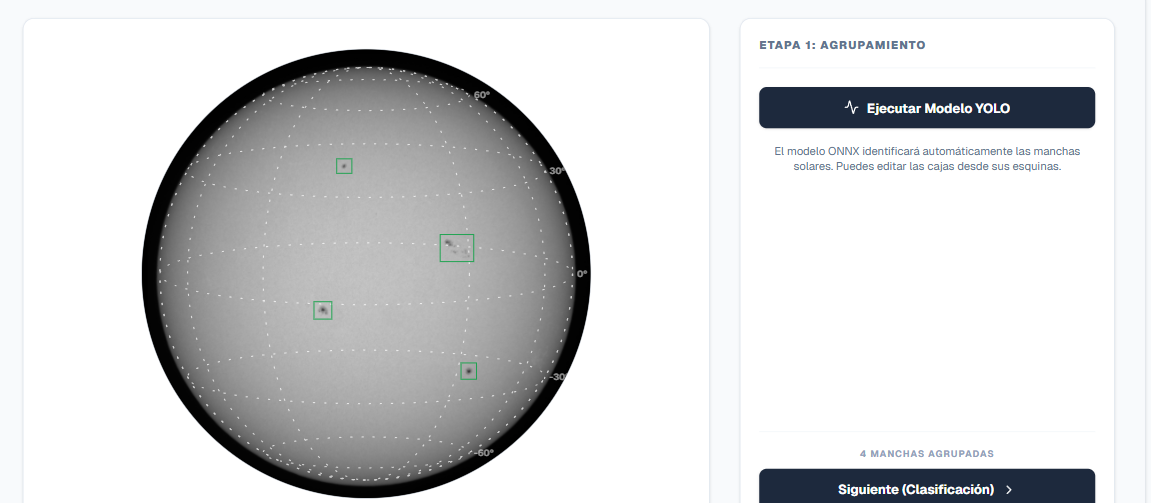
\includegraphics[height=0.75\textheight,width=0.96\linewidth,keepaspectratio]{web/yolo.png}
%     \vspace{0.08cm}
% \end{frame}

% \begin{frame}{Resultados: Plataforma Web (Clasificación con modelo jerárquica ConvNeXtv2a ONNX)}
%     \centering
%     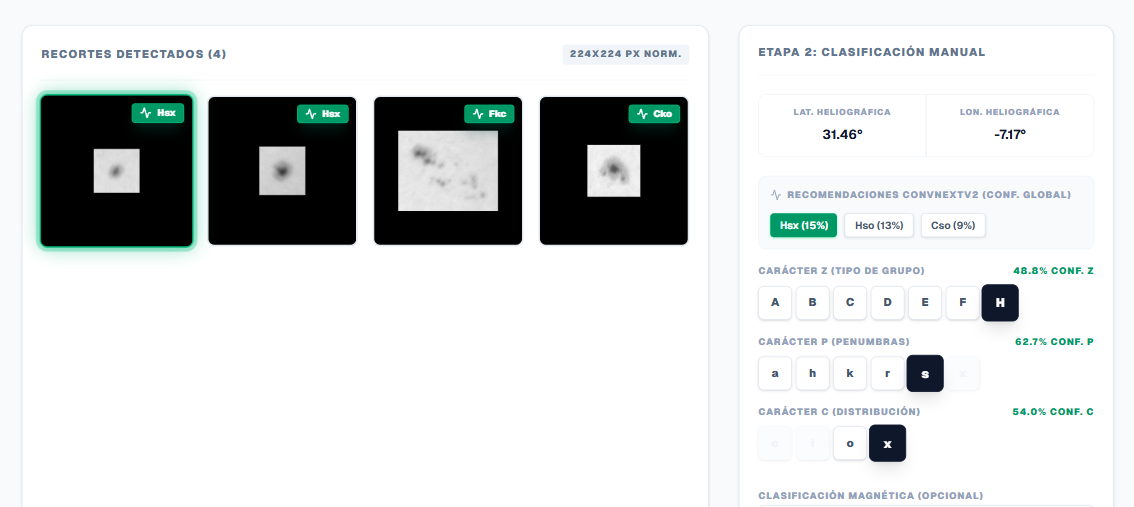
\includegraphics[height=0.75\textheight,width=0.96\linewidth,keepaspectratio]{web/convnext.png}
%     \vspace{0.08cm}
% \end{frame}

% \begin{frame}{Resultados: Plataforma Web (Diagrama de Spörer)}
%     \centering
%     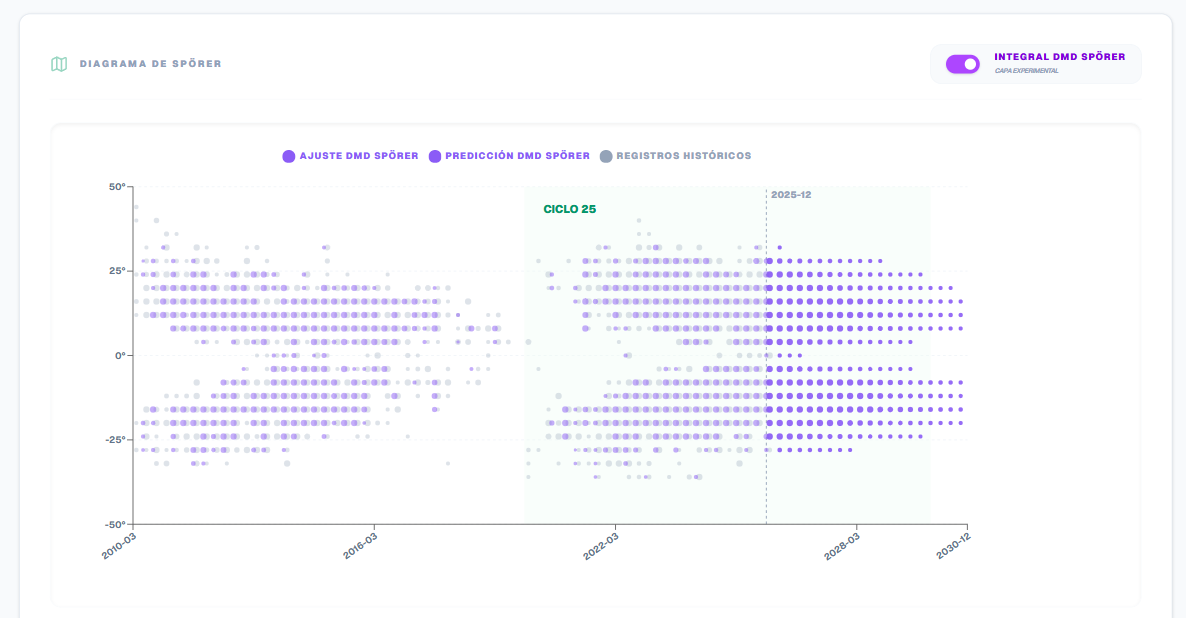
\includegraphics[height=0.75\textheight,width=0.96\linewidth,keepaspectratio]{web/butterfly.png}
%     \vspace{0.08cm}
% \end{frame}

% \begin{frame}{Resultados: Plataforma Web (Predicción SSN)}
%     \centering
%     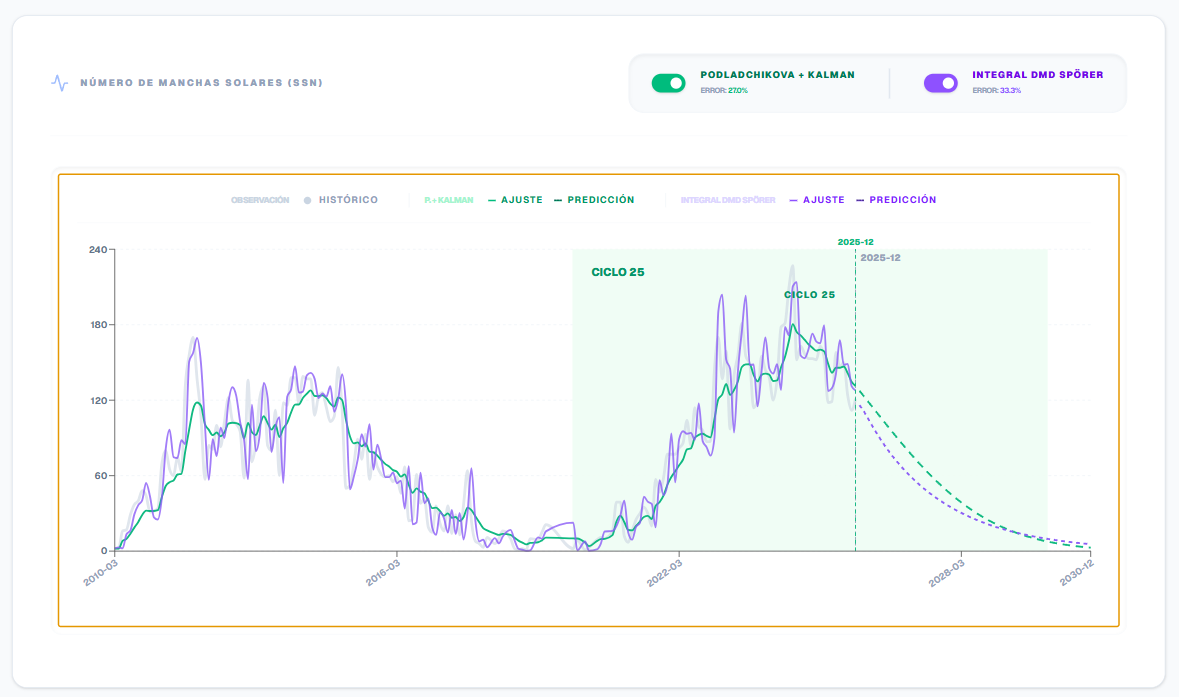
\includegraphics[height=0.75\textheight,width=0.96\linewidth,keepaspectratio]{web/ssn.png}
%     \vspace{0.08cm}
% \end{frame}


\section{Conclusões}

\begin{frame}{Conclusões}
    \small
    
     A articulação dos componentes de hardware e software permite extrair as seguintes conclusões:
    
    \begin{itemize}
        \scriptsize
        \item \textbf{Autonomia:} O dispositivo de aquisição local viabiliza o fluxo de dados sem dependência de conectividade externa constante.
        \item \textbf{Processamento na borda (ONNX):} A integração de modelos baseados em DMD e \textit{Deep Learning} valida a viabilidade técnica da execução de tarefas de classificação e análise preditiva em ambientes locais.
        \item \textbf{Monitoramento:} O \textit{framework} operacional unifica a captura e a análise automatizada de forma desacoplada.
    \end{itemize}

    \centering
    
    % Tabla de correspondencia con los objetivos específicos (OE)
    \renewcommand{\arraystretch}{1.2} 
    \begin{table}
        \centering
        \scriptsize
        \begin{tabular}{l|l|c}
            \toprule
            \textbf{Identificador} & \textbf{Descrição da Contribuição} & \textbf{Vínculo} \\ 
            \midrule
            \contrib{Contribuição 1} & Dispositivo de aquisição local & $\text{OE}_2$, $\text{OE}_5$ \\ 
            \contrib{Contribuição 2} & Base de dados rotulada de atividade solar & $\text{OE}_1$, $\text{OE}_2$ \\ 
            \contrib{Contribuição 3} & Modelo do Diagrama de Spörer baseado em DMD & $\text{OE}_4$ \\ 
            \contrib{Contribuição 4} & Modelo hierárquico de Deep Learning (Classificação) & $\text{OE}_3$ \\ 
            \bottomrule
        \end{tabular}
    \end{table}
\end{frame}


% \begin{frame}{Trabajo futuro y recomendaciones metodológicas}
%     \begin{columns}[c] % Alineación vertical centrada de las columnas
        
%         % Columna Izquierda: Imagen del equipo/telescopio
%         \begin{column}{0.40\textwidth}
%             \centering
%             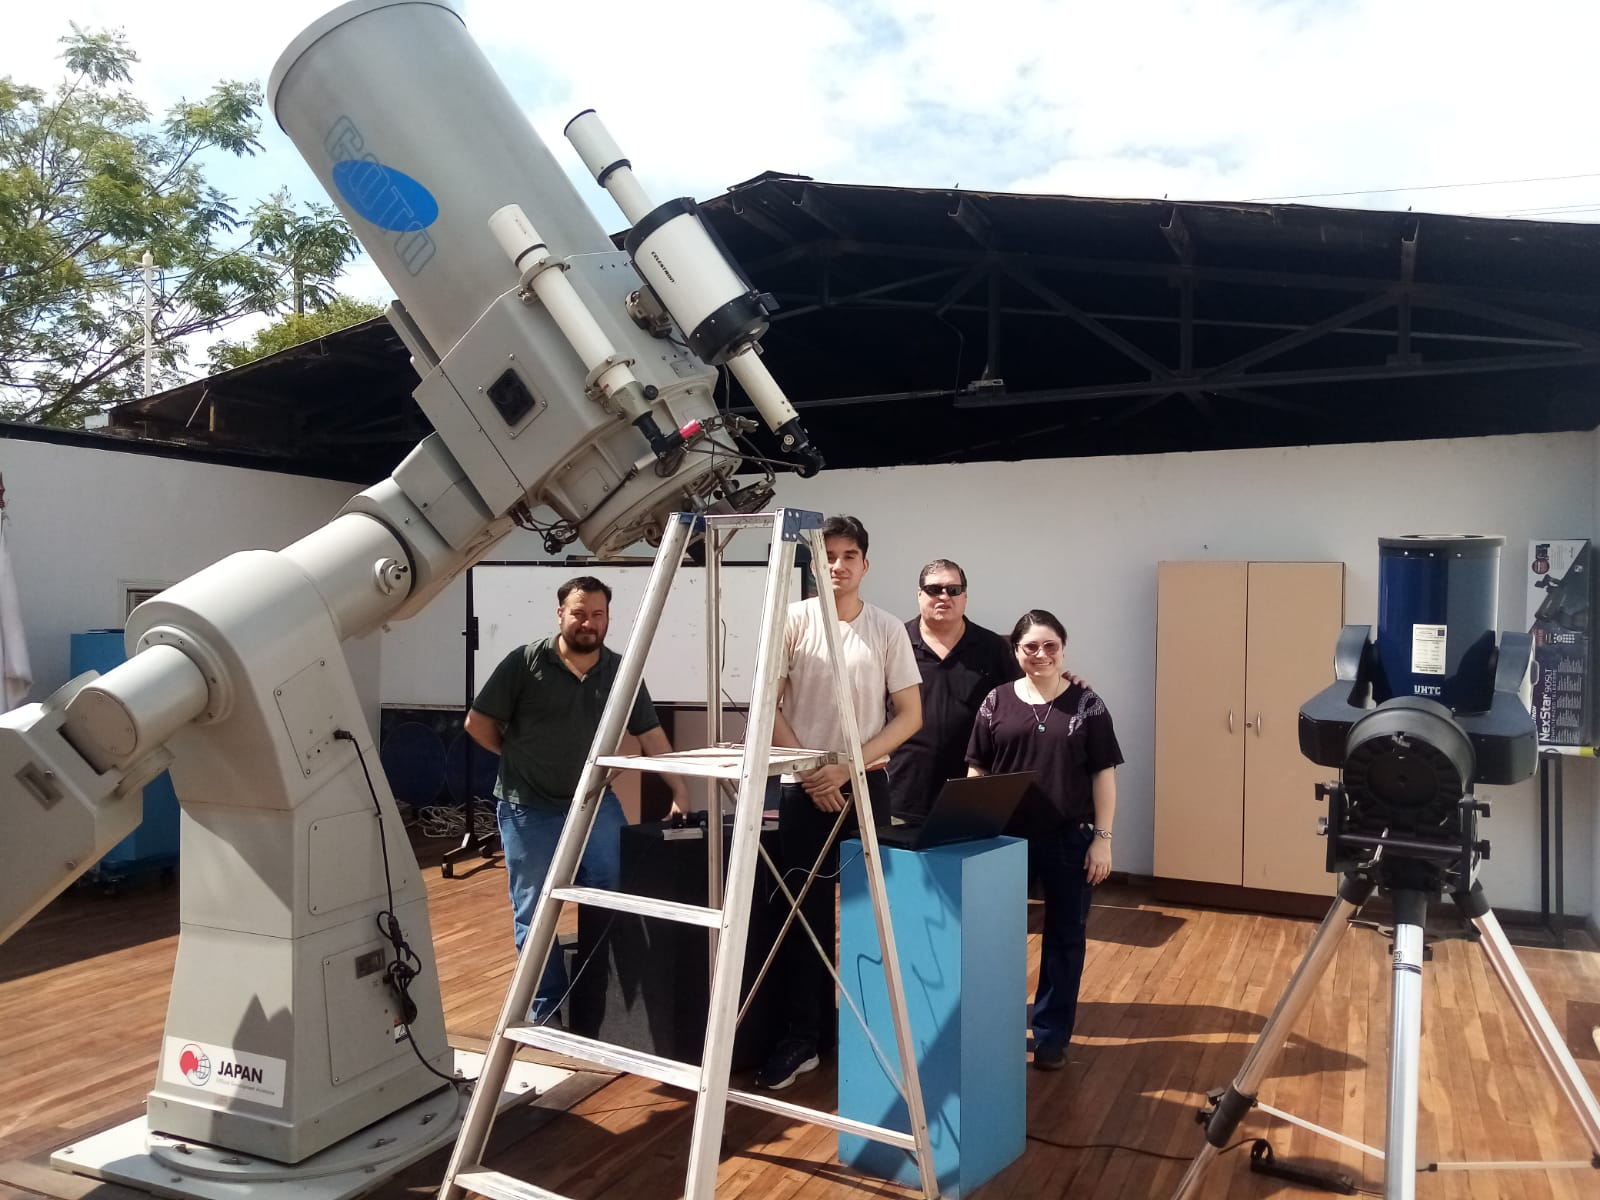
\includegraphics[height=0.75\textheight, width=\linewidth, keepaspectratio]{hw/telescope_team.jpg}
%         \end{column}
        
%         % Columna Derecha: Bloques de Trabajo Futuro y Recomendaciones técnicos y objetivos
%         \begin{column}{0.56\textwidth}
%             \scriptsize
            
%             % Bloque 1: Trabajo Futuro (Conversión de la tabla a un formato más compacto y limpio)
%             \begin{block}{Trabajo futuros}
%                 \begin{itemize}
%                     \item \textbf{Datos y Óptica:} Expandir campañas observacionales locales y automatizar las rutinas de enfoque y exposición del hardware.
%                     \item \textbf{Modelos y Validación:} Optimizar la ejecución en el borde mediante cuantización fina en ONNX y contrastar resultados con anotaciones manuales. Integrar un MPC en el DMD-Spörer para el refinamiento de error de reconstrucción.
                    
                    
%                 \end{itemize}
%             \end{block}
            
%             \vspace{0.1cm}
            
%             % Bloque 2: Recomendaciones (Incorporación rigurosa sobre el análisis de PCA)
%             \begin{block}{Recomendaciones metodológicas}
%                 \begin{itemize}
%                     \item \textbf{Análisis de sensibilidad en PCA:} Evaluar la reducción dimensional bajo análisis de sensibilidad estadístico para estimar el número óptimo de componentes principales.
%                     \item \textbf{Robustez del modelo:} Incrementar el volumen de observaciones locales con el fin de mitigar el sesgo y mejorar la transferencia de dominio del sistema.
                    
%                 \end{itemize}
%             \end{block}
            
%         \end{column}
%     \end{columns}
% \end{frame}

% --- Paquetes requeridos en el preámbulo si no están (para espaciado de tablas) ---
% \usepackage{array}

% --- FRAME 1: Línea Temporal - Proyectos de Álgebra Lineal Numérica ---
% \begin{frame}{Producción Científica: Álgebra Lineal Numérica}
%     \scriptsize
%     \centering
%     \begin{tabular}{r @{\hspace{0.8em}} c @{\hspace{0.8em}} l}
%         % Evento 1
%         \textbf{2025/06} & $\bullet$ & \textbf{X Encuentro de Investigadores del Paraguay} -- Asunción, \textit{Paraguay}. \\
%         & \vline & \textit{Un Marco Adaptativo con Descomposición en Modos Dinámicos con Control para el GMRES(m)}. \\
%         & \vline & \textcolor{llamativoMagenta}{Presentado} -- \textbf{Premio al mejor póster}. \\[0.4em]
        
%         % Evento 2
%         \textbf{2025/07} & $\bullet$ & \textbf{XLIV Congresso Nacional de Matemática Aplicada e Computacional (CNMAC)} -- Río de Janeiro, \textit{Brasil}. \\
%         & \vline & \textit{Adaptive System Identification for GMRES(m) Based on DMDc}. \\
%         & \vline & \textcolor{llamativoMagenta}{Presentado y Publicado} en \textit{Proceeding Series of the Brazilian Society of Computational and Applied Mathematics}. \\[0.4em]
        
%         % Evento 3
%         \textbf{2025/08} & $\bullet$ & \textbf{Encuentro de Matemáticas y Estadística Aplicadas a las CC. SS. y Económicas} -- Bogotá, \textit{Colombia}. \\
%         & \vline & \textit{Identificación de sistema para el GMRES(m)}. \\
%         & \vline & \textcolor{llamativoMagenta}{Presentado}. \\[0.4em]

%         % Evento 4
%         \textbf{2026/04} & $\bullet$ & \textbf{XLV Congresso Nacional de Matemática Aplicada e Computacional (CNMAC)} -- São Paulo, \textit{Brasil}. \\
%         & \vline & \textit{Solving the Mimetic Pressure Poisson Equation in a 2D Flow Using DMDc–LQR–LGMRES($m,\ell$)}. \\
%         & \vline & \textcolor{deepred}{Sometido}. \\[0.5em]
        
%         % Evento 5
%         \textbf{2026/06} & $\bullet$ & \textbf{X Pan American Workshop in Applied and Computational Mathematics (PANAM)} -- Quito, \textit{Ecuador}. \\
%         & \vline & \textit{A Control-Oriented Mimetic Solver for the Pressure Poisson Equation in a 2D Lock-Exchange Flow}. \\
%         & \vline & \textcolor{llamativoMagenta}{Presentado}.
%     \end{tabular}
% \end{frame}

% % --- FRAME 2: Línea Temporal - Presentaciones Inspiradas en la Tesis ---
% \begin{frame}{Producción Científica: Aplicaciones de la Tesis}
%     \scriptsize
%     \centering
%     % Se usa p{10cm} para forzar el ajuste de línea automático en títulos muy extensos (como el de las JJII-UNA)
%     \begin{tabular}{r @{\hspace{0.8em}} c @{\hspace{0.8em}} p{10cm}}
%         % Evento 1
%         \textbf{2026/05} & $\bullet$ & \textbf{DEEP-DIVE-FIUNA} -- Asunción, \textit{Paraguay}. \\
%         & \vline & \textit{Detección y Clasificación Jerárquica Zürich--McIntosh de Manchas Solares}. \\
%         & \vline & \textcolor{llamativoMagenta}{Presentado}. \\[0.5em]
        
%         % Evento 2
%         \textbf{2026/06} & $\bullet$ & \textbf{Ibero--American Conference on Artificial Intelligence (IBERAMIA)} -- Asunción, \textit{Paraguay}. \\
%         & \vline & \textit{Cascaded Deep Learning Framework for Zürich--McIntosh Sunspot Classification}. \\
%         & \vline & \textcolor{deepred}{Sometido}. \\[0.5em]
        
%         % Evento 3
%         \textbf{2026/06} & $\bullet$ & \textbf{Jornadas de Jóvenes Investigadores de la Universidad Nacional de Asunción (JJI-UNA)} -- Asunción, \textit{Paraguay}. \\
%         & \vline & \textit{Desarrollo de un Prototipo de Procesamiento Local para la Detección, Clasificación y Análisis Predictivo de Manchas Solares mediante Visión Computacional e Inteligencia Artificial}. \\
%         & \vline & \textcolor{deepred}{Sometido}. \\[0.5em]
        
%         % Evento 4
%         \textbf{2026/06} & $\bullet$ & \textbf{IEEE-ARGENCON} -- Córdoba, \textit{Argentina}. \\
%         & \vline & \textit{Local AI Prototype for Sunspot Detection and Analysis}. \\
%         & \vline & \textcolor{deepred}{Sometido}.
%     \end{tabular}
% \end{frame}

\begin{frame}
    \centering
    \vspace{-0.15cm}
    {\LARGE\textbf{\color{rojo-oscuro} Muito Obrigado!}}

    \vspace{0.35cm}
    \begin{columns}[c]
        \begin{column}{0.48\textwidth}
            \centering
            
\includegraphics[height=3.8cm,keepaspectratio]{qr/web.png}\\[4pt]
            {\scriptsize\textbf{Plataforma Web}}\\[1pt]
            {\tiny\color{black!75} Demonstração interativa e visualizador web.}\\[1pt]
            {\tiny\url{https://sunspot-page-app.vercel.app}}
        \end{column}
        \begin{column}{0.48\textwidth}
            \centering
            
\includegraphics[height=3.8cm,keepaspectratio]{qr/repo.png}\\[4pt]
            {\scriptsize\textbf{Repositório do Projeto}}\\[1pt]
            {\tiny\color{black!75} Código-fonte, modelos ONNX e datasets.}\\[1pt]
            {\tiny\url{https://github.com/carlobeni/sunspot-page-app}}
        \end{column}
    \end{columns}
\end{frame}

% \begin{frame}{Anexo 1: Conflicto de operatividad}
    
%     \vspace{0.2cm} % Margen inicial sutil debajo del título del frame

%     % [c] fuerza a que TODOS los elementos de las columnas se alineen horizontalmente por su centro geométrico
%     \begin{columns}[c]
        
%         % Columna 1: SIDC / USET
%         \begin{column}{0.31\textwidth}
%             \centering
%             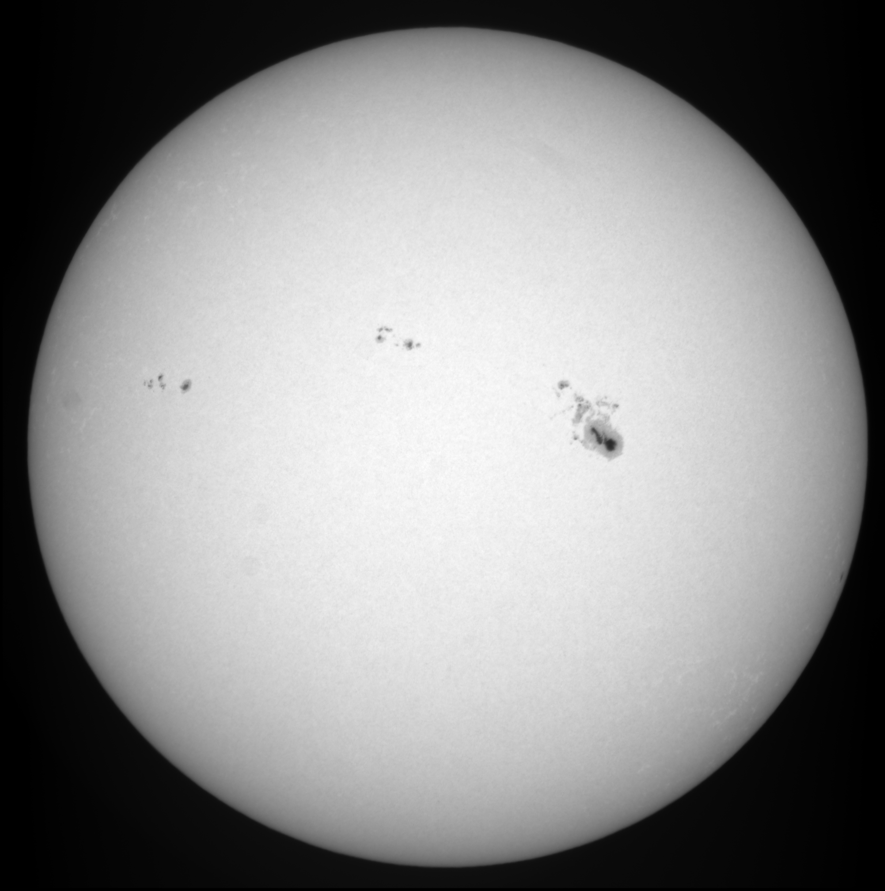
\includegraphics[height=0.5\textheight, width=\linewidth, keepaspectratio]{data/wl.png}\par
%             \vspace{0.08cm}
%             {\tiny Luz Blanca del 2025-05-06\\(Terrestre SIDC/USET[6])}
%         \end{column}
        
%         % Columna 2: SDO / NASA
%         \begin{column}{0.31\textwidth}
%             \centering
%             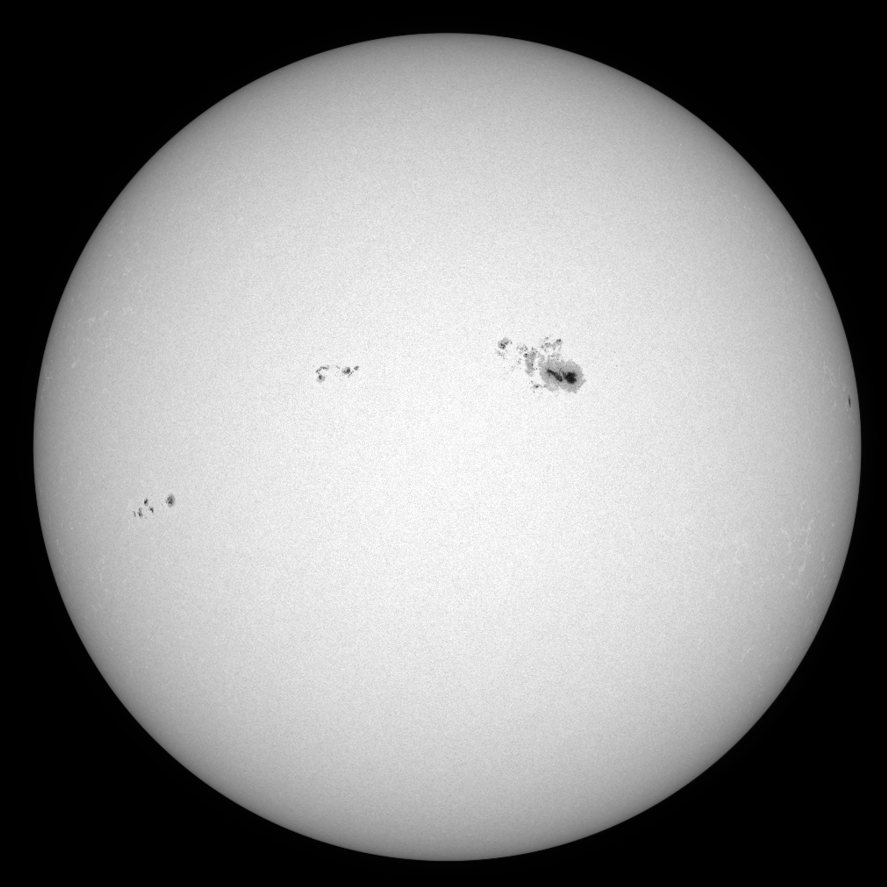
\includegraphics[height=0.5\textheight, width=\linewidth, keepaspectratio]{data/hmi.png}\par
%             \vspace{0.08cm}
%             {\tiny Imagen HMI del 2025-05-06\\(Satélite SDO/NASA [13])}
%         \end{column}
        
%         % Columna 3: Nota técnica en cuadro de bordes curvos y fondo magenta
%         \begin{column}{0.34\textwidth}
%             % Configuración local de colores para la caja curva
%             \setbeamercolor{cajaMagenta}{fg=white, bg=llamativoMagenta}
            
%             \begin{beamercolorbox}[wd=\linewidth, rounded=true, sep=6pt]{cajaMagenta}
%                 \scriptsize
%                 \textbf{Efecto de Paralaje}
%                 \vspace{0.1cm}
                
%                 El emparejamiento SDO-SIDC introduce un paralaje geométrico debido a la diferencia de perspectiva espacial-terrestre.
%                 \vspace{0.12cm}
                
%                 Sin embargo, al no haber cambios morfológicos significativos, este efecto se considera \textbf{despreciable} para la clasificación.
%             \end{beamercolorbox}
%         \end{column}
        
%     \end{columns}

%     \vfill % Empuja de forma exacta y limpia las referencias al límite inferior de la diapositiva

%     {\tiny\color{gray}
%     [6] Royal Observatory of Belgium, “Understanding Solar Activity Telescopes (USET) report,” 2025.\par\vspace{0.03cm}
%     [13] NASA Goddard Space Flight Center, “Helioseismic and Magnetic Imager (HMI) aboard the Solar Dynamics Observatory (SDO),” 2025.\par}
% \end{frame}


% \begin{frame}{Anexo 2: Costos del Prototipo}
%     \centering
%     \vfill

%     \scriptsize \textbf{Presupuesto Referencial de Componentes del Prototipo}
%     \vspace{0.1cm}

%     % Configuración de tabla compacta y estética para Beamer sin la columna de cantidad
%     \renewcommand{\arraystretch}{1.2}
%     \setlength{\tabcolsep}{12pt} % Un poco más de separación al tener menos columnas
%     \begin{table}
%         \centering
%         \scriptsize
%         \begin{tabular}{lrr}
%             \toprule
%             \textbf{Componente} & \textbf{Precio (USD)} & \textbf{Precio (PYG)} \\
%             \midrule
%             Raspberry Pi 5 8 GB & 190 & 1.160.520 \\
%             Módulo active cooler para Raspberry Pi 5 & 13 & 79.404 \\
%             Cámara ZWO ASI174MM Mini & 432 & 2.638.656 \\
%             Filtro solar Herschel wedge Lunt 1.25'' con ND3 & 308 & 1.881.264 \\
%             Pantalla OLED 0.96'' 128x64 & 9 & 54.972 \\
%             Impresión 3D de carcasa y soporte & 4 & 24.432 \\
%             \midrule
%             % Fila de TOTAL unificada y limpia con el fondo gris
%             \rowcolor{black!12} \textbf{Total} & \textbf{956} & \textbf{5.839.248} \\
%             \bottomrule
%         \end{tabular}
%     \end{table}

%     \vspace{0.3cm}

%     % Breve comentario cualitativo debajo de la tabla (1 USD = 6108 PYG)
%     \begin{minipage}{0.85\linewidth}
%         \centering
%         \scriptsize\itshape
%         La inversión total de hardware asciende a \textbf{5.839.248 PYG} (956 USD), consolidando una arquitectura basada en sistemas embebidos de bajo costo y alto rendimiento óptico para el procesamiento solar local.
%     \end{minipage}

%     \vfill
% \end{frame}

% \begin{frame}{Anexo 3: Montaje Completo}
%     \centering
%     \begin{columns}[c]
%         \begin{column}{0.48\linewidth}
%             \centering
%             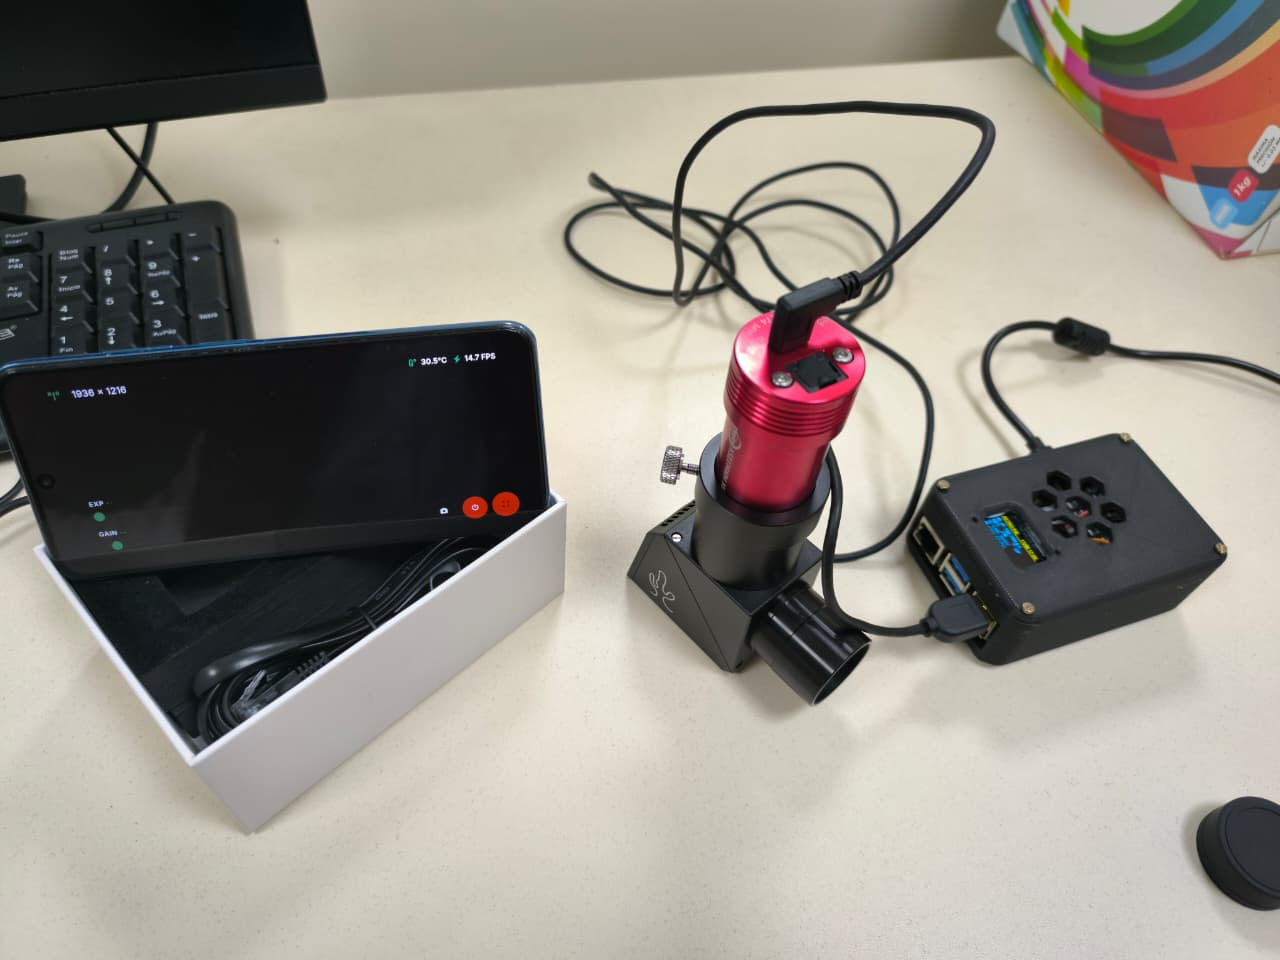
\includegraphics[height=0.6\textheight,width=\linewidth,keepaspectratio]{hw/integrated.jpeg}
%         \end{column}
%         \hfill % or just let columns handle spacing
%         \begin{column}{0.48\linewidth}
%             \centering
%             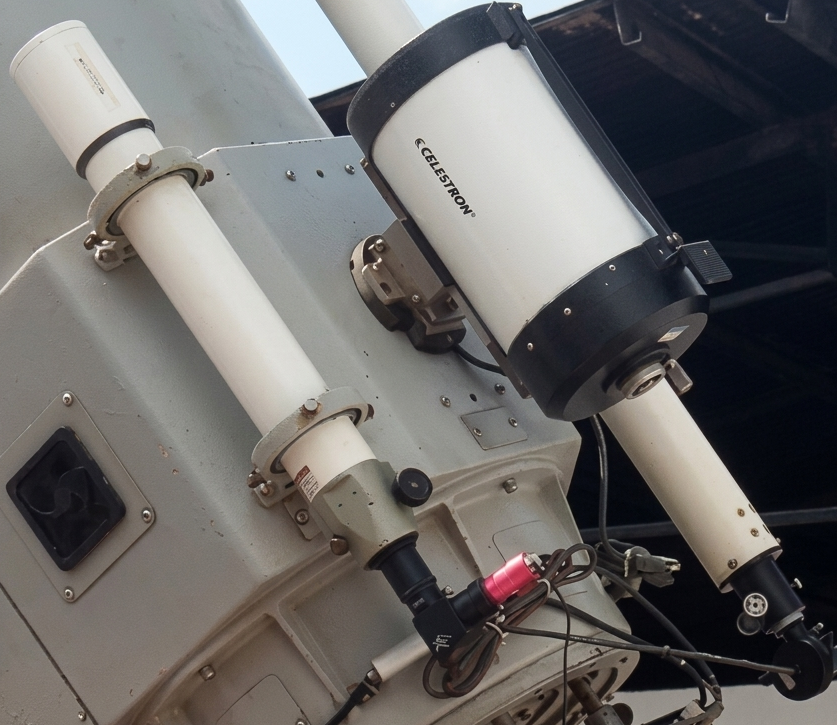
\includegraphics[height=0.6\textheight,width=\linewidth,keepaspectratio]{hw/telescopio_zoom.png}
%         \end{column}
%     \end{columns}
% \end{frame}

% \begin{frame}{Anexo 4: Diseño CAD (SolidWorks)}
%     \centering
%     \begin{columns}[c] % Changed from [T] to [c] for vertical centering
%         \begin{column}{0.32\linewidth}
%             \centering
%             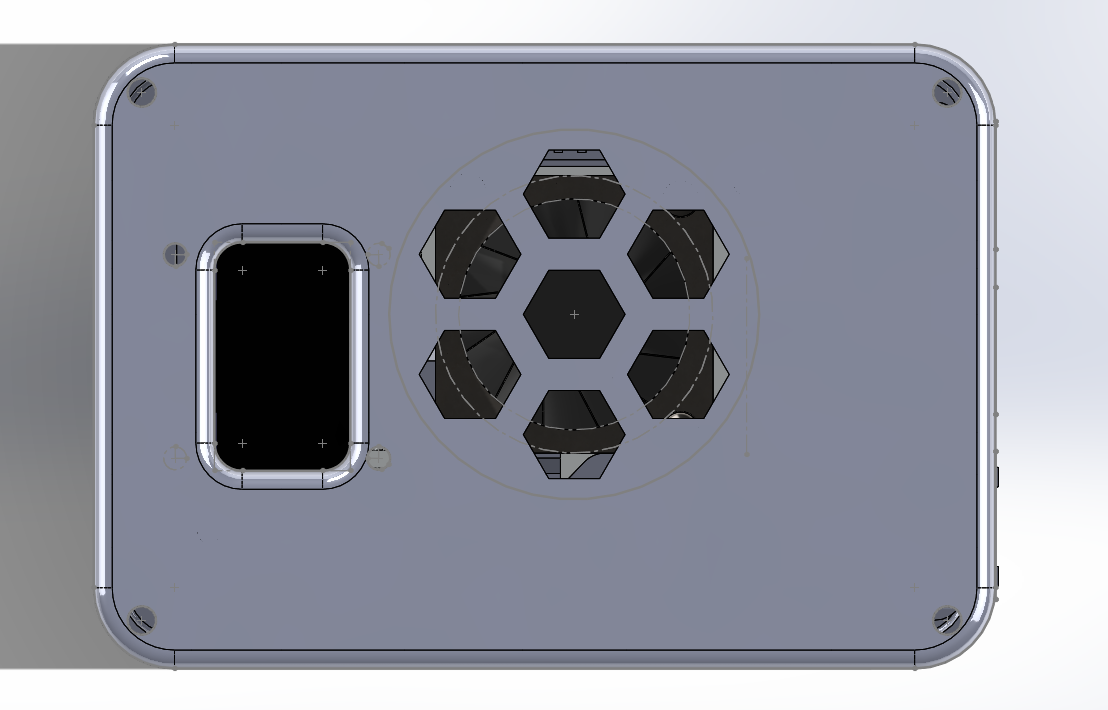
\includegraphics[width=\linewidth]{cad/case_lid.png}
%             %{\tiny Matriz de confusión para Z.}
%         \end{column}
%         \begin{column}{0.32\linewidth}
%             \centering
%             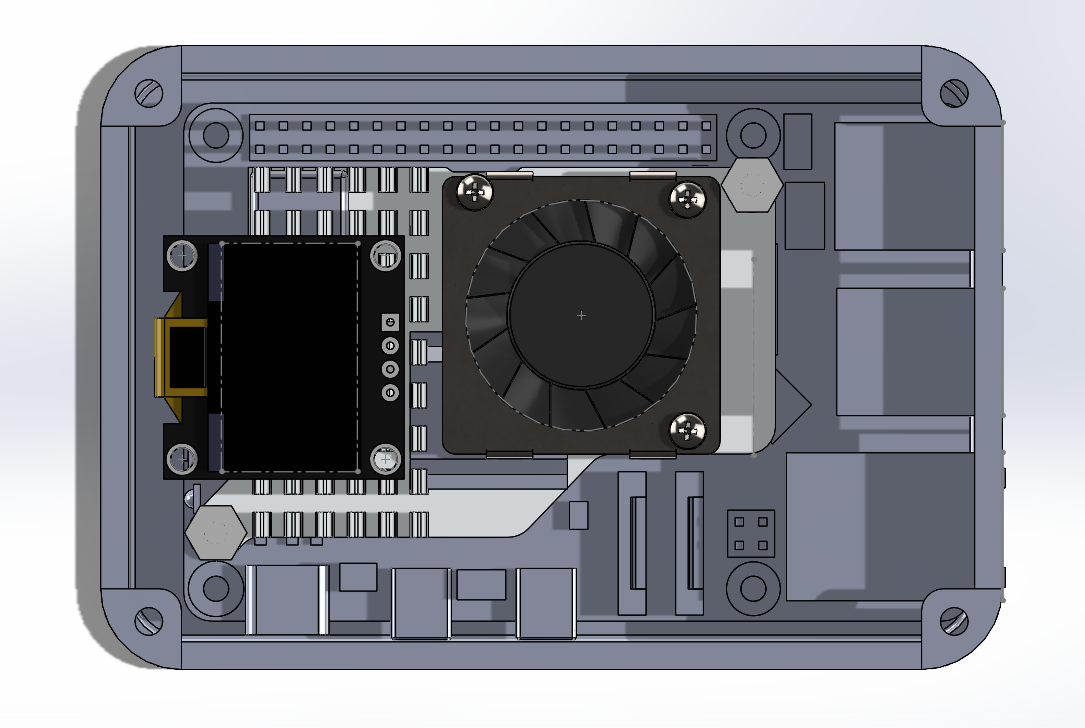
\includegraphics[width=\linewidth]{cad/case_open.png}
%             %{\tiny Matriz de confusión para P.}
%         \end{column}
%         \begin{column}{0.32\linewidth}
%             \centering
%             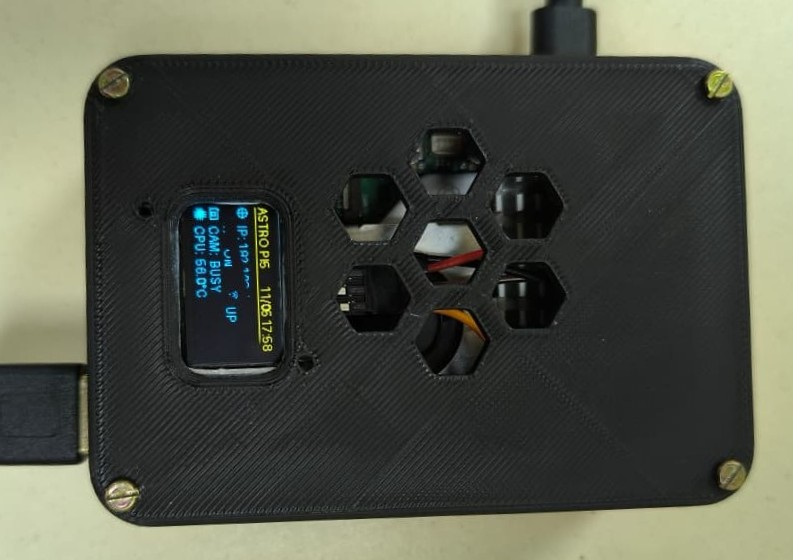
\includegraphics[width=\linewidth]{hw/obs_module.jpeg}
%             %{\tiny Matriz de confusión para C.}
%         \end{column}
%     \end{columns}
% \end{frame}

% \begin{frame}{Anexo 5: Plataforma Web}
%     \centering
%     
\includegraphics[height=0.75\textheight,width=0.96\linewidth,keepaspectratio]{qr/web.png}
%     \vspace{0.08cm}
% \end{frame}

\end{document}